\documentclass[a4paper, 16pt]{article}
\usepackage[utf8]{inputenc}
\usepackage{cmap}
\usepackage[T2A]{fontenc}
\usepackage[russian]{babel}
\usepackage[left=2cm, right=1.5cm, top=1.5cm, bottom=1.5cm]{geometry}
\usepackage{ragged2e}
\usepackage{graphicx}
\usepackage{float}
\usepackage{listings}
\usepackage{fancyhdr}
\usepackage{ulem}
\usepackage{enumitem}
\usepackage{tikz}
\usepackage{algorithm}
\usepackage[noend]{algpseudocode}

\usepackage{xcolor}
\usepackage{hyperref}

\usepackage{amsmath}
\DeclareMathOperator{\Det}{Det}
\DeclareMathOperator{\dom}{dom}
\DeclareMathOperator{\capl}{\cap}
\DeclareMathOperator{\Tr}{Tr}
\DeclareMathOperator{\Diag}{Diag}
\DeclareMathOperator{\Rk}{Rk}
\DeclareMathOperator{\grad}{grad}
\DeclareMathOperator{\Dim}{dim}
\DeclareMathOperator{\Transp}{Transp}
\DeclareMathOperator*{\argmax}{arg\,max}
\DeclareMathOperator*{\argmin}{arg\,min}

 % Цвета для гиперссылок
\definecolor{linkcolor}{HTML}{799B03} % цвет ссылок
\definecolor{urlcolor}{HTML}{799B03} % цвет гиперссылок

\hypersetup{pdfstartview=FitH,  linkcolor=linkcolor, urlcolor=urlcolor, colorlinks=true}

\newcommand{\theorem}[1]{\begin{center}\fbox{\begin{minipage}{\textwidth-1cm}#1 \end{minipage}}\end{center}}
\newcommand{\Sym}{\mathbb{S}}
\newcommand{\R}{\mathbb{R}}

\usepackage{amsfonts, amsthm, mathtools, amssymb, icomma, units, mathrsfs}
\usepackage{amssymb}

\fancypagestyle{first}{
    \cfoot{1}
    \renewcommand{\footrulewidth}{0 mm}
    \renewcommand{\headrulewidth}{0 mm}
}

\fancypagestyle{plain}{
    \renewcommand{\headrulewidth}{0 mm}
    \renewcommand{\footrulewidth}{0.3 mm}
    \cfoot{\normalsize\thepage}
    \lfoot{
        Непрерывная оптимизация.
        Экзамен
    }
    \rfoot{171 группа}
}

\begin{document}
    \begin{titlepage}
        \centering
        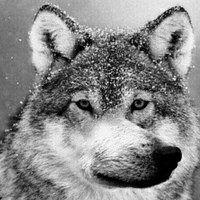
\includegraphics[width=10cm]{images/wolfe.jpg} \\
        \begin{flushright}
            \textit{\large Homo homini lupus est.}
        \end{flushright}
        \vspace{0.5cm}
        \Large{ПМИ ФКН ВШЭ} \\
        \huge{\bf Непрерывная оптимизация. Экзамен.} \\
        \vspace{0.2cm}
        \Large{171 группа}
        \vfill
        \Large{Июнь 2020}
    \end{titlepage}
    \thispagestyle{first}
    \newpage
    \setcounter{tocdepth}{2}
	\tableofcontents
	\newpage
	\pagestyle{plain}

    \section{Теоретический минимум}
    \subsection{Определение линейной/сублинейной/суперлинейной скорости сходимости. Пример последовательности для каждого класса. @mercivboku}

    \textbf{Невязку} можно определять по-разному, в дальнейшем будут использоваться все виды определений:
\begin{enumerate}
    \item $r_k = \|x_k - x_{opt}\|$
    \item $r_k = |f(x) - f_{opt}|$
    \item $r_k = \|\nabla f(x_k)\|$
\end{enumerate}
Теперь рассмотрим различные виды сходимости. \\
Опреления из лекции:

$\{r_k\}$ сходится \textbf{Q-сублинейно}, если \[\varlimsup\limits_{k\to\infty} \dfrac{r_{k+1}}{r_k} = 1.\]

$\{r_k\}$ сходится \textbf{Q-линейно}, если $\exists c\in(0; 1): $
\[\varlimsup\limits_{k\to\infty} \dfrac{r_{k+1}}{r_k} = c.\]

$\{r_k\}$ сходится \textbf{Q-суперлинейно}, если \[\varlimsup\limits_{k\to\infty} \dfrac{r_{k+1}}{r_k} = 0.\]


$\{r_k\}$ сходится \textbf{Q-квадратично}, если $\exists M>0:$ \[r_{k+1} \leq M r_k^2\ \ \ \forall k \geq k_0\]

$\{r_k\}$ сходится \textbf{R-линейно}, если $\exists$ монотонная последовательность $\{\eta_k\}$: $r_{k+1} \leq \eta_k$ и $\{\eta_k\}$ сходится Q-линейно.
\bigskip

Определения из конспекта:\\
$\{r_k\}$ сходится \textbf{q-линейно} с параметром $q\in (0; 1)$, если существует такое $C > 0$, что

\[r_k \leq Cq^k\ \ \ \forall k \geq m.\]

При этом если существует хотя бы одно такое $q$, то последовательность сходится \textbf{линейно}.

\underline{Пример:} $r_k = \dfrac{1}{3^k}$ и $r_k = \dfrac{4}{3^k}$ сходятся линейно с любым параметром $q \in \left[\dfrac{1}{3}; 1\right)$. При этом константа линейной сходимости (точная нижняя грань множества из всех $q$) для обеих последовательностей равна $\dfrac{1}{3}$.

$\{r_k\}$ сходится \textbf{сублинейно}, если $\{r_k\}$ сходится к 0, но не обладает линейной сходимостью. Если же, наоборот, $\{r_k\}$ обладает линейной сходимостью, и константа линейной сходимости равна 0, говорят, что $\{r_k\}$ сходится \textbf{суперлинейно} или \textbf{сверхлинейно}.

\underline{Пример:} Последовательность $r_k = \dfrac{1}{k}$ не обладает линейной сходимостью, однако сходится к 0, значит, обладает сублинейной сходимостью. \\
Последовательность $r_k = \dfrac{1}{3^{k^2}}$ сходится линейно, при этом параметр сходимости приближается к 0 сколь угодно близко, значит, константа линейной сходимости равна 0, значит, данная последовательность сходится также суперлинейно.



    \subsection{Условия Армихо и Вульфа для неточной одномерной оптимизации. Процедура бэктрекинга. @mercivboku}

    Введем некоторые обозначения:\\
$x_{k+1} = x_k + \alpha_k d_k, \ x_k, d_k \in \mathbb{R}^n$\\
$\varphi(\alpha) = f(x_k + \alpha_k d_k)$, также есть примерное приближение: $\varphi(\alpha) \approx f(x_k) + \alpha \nabla f(x_k)^Td_k$\\
$\varphi(\alpha) \to \min\limits_{\alpha}$\\
$\nabla f(x_k)^Td_k = \varphi'(0) < 0$\\

\textbf{Условие Армихо}:
\begin{itemize}
    \item $\varphi(\alpha_k) \leq \varphi(0) + c_1\alpha_k\varphi'(0),\ \ c_1 \in (0; 1)$
\end{itemize}
Нужно для этого: $\varphi(0) - \varphi(\alpha_k) = f(x_k) - f(x_k + \alpha_k d_k)\geq -\alpha_k(c_1\varphi'(0))>0$

Хотим делать большие шаги, пока функция тоже меняется сильно. $c_1$ должно быть близким к 0, чем ближе, тем больше шаги мы разрешаем.
\bigskip

\textbf{Условия Вульфа:}
\begin{itemize}
    \item $\varphi'(\alpha_k) \geq c_2 \varphi'(0)$ -- слабое условие (помним, что $\varphi'(0) < 0$)
    \item $|\varphi'(\alpha_k)| \leq c_2 |\varphi'(0)|, \ c_2 \in (0, 1)$ -- сильное условие
    \item  $\varphi(\alpha_k) \leq \varphi(0) + c_1\alpha_k\varphi'(0),\ \ c_1 \in (0; 1)$ (условие Армихо, иногда он включал его в Вульфа, иногда нет, но всегда, когда рассматриваем Вульфа, разумно, чтобы Армихо тоже было выполнено)
\end{itemize}
Чем ближе $c_2$ к 0, тем ближе мы к локальному минимуму (тем больше берем шаг), чем ближе $c_2$ к 1, тем гибче (можем взять маленький шаг).
\bigskip

\textbf{Утверждение.} Если $\varphi'(0) < 0,\ \varphi(\alpha) > -\infty\ \forall \alpha,\ 0<c_1\leq c_2<1$, то $\exists\ \alpha_*$, которое удовлетворяет условиям Армихо и Вульфа (в любой форме).
\bigskip

\textbf{Алгоритм Backtracking:}
\begin{algorithm}[H]
    \begin{algorithmic}[1]
        \Procedure{backtracking}{$\alpha_{start},\ \beta,\ \varphi_k:\mathbb{R_+}\to\mathbb{R}$}
        \State $\alpha \gets \alpha_{start}$
        \While{$\varphi_k(\alpha) > \varphi(0) + c_1\alpha\varphi'_k(0)$}
            \State $\alpha \gets \beta\alpha$
        \EndWhile
        \State \Return $\alpha$
        \EndProcedure
    \end{algorithmic}
\end{algorithm}

    \subsection{Общее определение производной функции (через линейное отображение). Основные свойства производной (правила суммы, произведения и композиции). Определения второй производной, градиента и гессиана. @mercivboku}

    Для начала вспомним самое начало:
Для функции одной переменной $f: \mathbb{R} \to \mathbb{R}$ ее производная в точке $x$ обозначается $f'(x)$ и определяется из равенства:

$$f(x+h) = f(x) + f'(x)h + o(h)\ \text{для всех достаточно малых}\ h.$$

То есть при некоторой зафиксированной точке $x$ мы хотим приблизить изменение функции $f(x + h) - f(x)$ в окрестности нашего $x$ с помощью линейной функции по $h$, и $f'(x)h$ -- наилучший способ это сделать.
\bigskip

\textbf{Определение.} Пусть $x\in X$ -- внутренняя точка множества $X$ и пусть $L : U \to V$ -- линейный оператор. Будем говорить, что фукнция $f$ \textit{дифференцируема в точке x с производной L}, если для всех достаточно малых $h \in U$ справедливо следующее разложение:

$$f(x+h) = f(x) + L[h] + o(\|h\|).$$

Будем обозначать производную символом $df(x),$ также валидны символы $Df(x)[h]$ или $df(x)[h]$, где $h = \Delta x$ -- приращение.
\bigskip

\textbf{Определение.} Производная функции в точке $x$ --  это линейный оператор $df(x)$, который лучше всего аппроксимирует приращение функции:

$$f(x+h) - f(x) \approx Df(x)[h].$$

\textbf{Свойства производной}:

Пусть $U$ и $V$ -- векторные пространства, $X$ -- подмножество $U$, $x\in X$ -- внутренняя точка $X$. Справедливы следующие свойства:

\begin{itemize}
    \item (Линейность) Пусть $f : X \to V$ и $g : X \to V$ -- функции. Если $f$ и $g$ дифференцируемы в точке $x$, а $c_1,\ c_2\in\mathbb{R}$ -- числа, то функция $(c_1f + c_2g)$ также дифференцируема в точке $x$ и ее производная:

    $$d(c_1f + c_2g)(x) = c_1df(x) + c_2dg(x).$$

    \item (Правило произведения) Пусть $\alpha: X \to \mathbb{R}$ и $f : X \to V$ -- функции. Если $\alpha$ и $f$ дифференцируемы в точке $x$, то функция $\alpha f$ также дифференцируема в точке $x$ и

    $$D(\alpha f)(x)[h] = (D \alpha(x)[h])f(x) + \alpha(x)Df(x)[h].$$


    \item (Правило композиции) Пусть $Y$ -- подмножество $V$, $f : X \to Y$ -- функция. Также пусть $W$ -- векторное пространство, $g : Y \to W$ -- функция. Если $f$ дифференцируема в точке $x$, и $g$ дифференцируема в точке $f(x)$, то их композиция $(g \circ f) : X \to W$ (определяем как $g(f(x))$) дифференцируема в точке $x$, и

    $$D(g \circ f)(x) = Dg(f(x))[df(x)] $$
\end{itemize}
\bigskip

\textbf{Определение.} В случае $U = \mathbb{R}^n$ линейную функцию $Df(x)[h]$ можно представить с помощью скалярного произведения с некоторым вектором:

$$Df(x)[h] = \langle a_x, h\rangle,\ \ \ \text{где}\ a_x\in\mathbb{R}^n\text{ -- разный для каждого } x. $$

Вектор $a_x$ называется \textit{градиентом}  функции $f$ в точке $x$ и обозначается $\nabla f(x)$.

Отметим, что в стандартном базисе он представляется в привычном нам виде вектора (столбца) частных производных:

$$\nabla f(x) = \left(\dfrac{\partial f}{\partial x_1}(x),\ldots,\dfrac{\partial f}{\partial x_n}(x)\right)\in \mathbb{R}^n.$$
\bigskip

\textbf{Определение.} Пусть функция $f: X \to V$ дифференцируема в каждой точке $x\in X \subseteq U$. \\
Рассмотрим производную функции $f$ при фиксированном приращении $h_1\in U$ как функцию от $x$:

$$g(x) = Df(x)[h_1].$$

Если для функции $g$ в некоторой точке $x$ существует производная, то она называется \textit{второй производной} функции $f$ в точке $x$:

$$D^2 f(x) [h_1, h_2] := Dg(x)[h_2].$$
\bigskip

\textbf{Определение.} Вторую производную для функций $f :  \mathbb{R}^n\to\mathbb{R}$ также можно представить в виде матрицы:
$$D^2f(x)[h_1, h_2] = \langle H_xh_1, h_2\rangle,\ \ H_x\in\mathbb{R}^{n\times m}.$$

Матрица $H_x$ называется \textit{гессианом} функции $f$ в точке $x$ и обозначается $\nabla^2f(x).$ В стандартном базисе это матрица частных производных:

$$\nabla^2f(x) = \left(\dfrac{\partial^2 f}{\partial x_i\partial x_j}(x)\right)_{i,j = 1}^n.$$

Для дважды непрерывно дифференцируемой функции гессиан симметричен.

    \subsection{Классы липшицевых функций, гладких выпуклых и сильно выпуклых функций. Соответствующие глобальные верхние и нижние оценки на функцию. Примеры функций для каждого класса. @mercivboku}

    \textbf{Липшициевость:}\\
Обозначение: $f\in C^{k, m}_L$. Пусть $m\leq k,\ L > 0$ -- константа Липшица, тогда:
$$f\in C^{k, m}_L \Leftrightarrow \left[
\begin{array}{ccc}
    & f\in C^k,                                                  \\
    & \|\nabla^mf(y)-\nabla^mf(x)\|\leq L\|y - x\|\ \forall x, y \\
\end{array}
\right.$$
В частности, если $f\in C^{1, 1}_L$, то верно

$$\|\nabla f(y)-\nabla f(x)\|\leq L\|y - x\|\ \  \Leftrightarrow\ \  \begin{array}{ccc}
                                                                         f(y) \leq f(x) + \nabla f(x)^T(y-x) + \dfrac{L}{2}\|y - x\|^2 \\
                                                                         f(y) \geq f(x) + \nabla f(x)^T(y-x) - \dfrac{L}{2}\|y - x\|^2
\end{array}
$$

\begin{figure}[H]
    \centering
    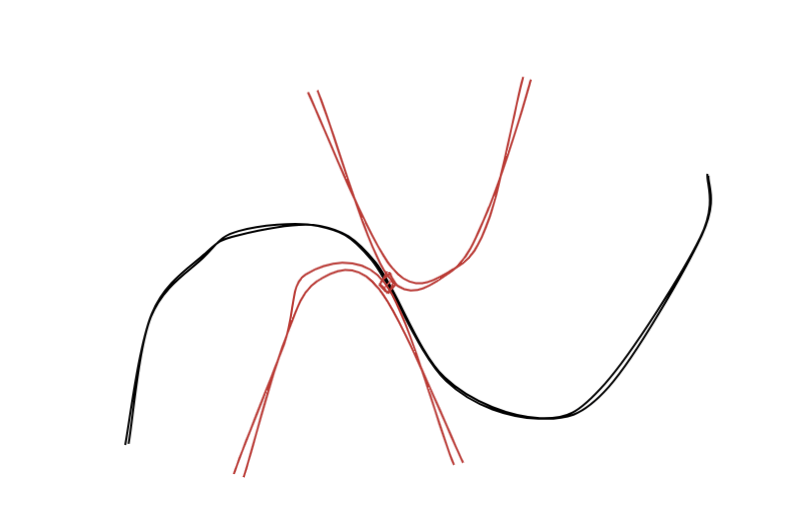
\includegraphics[width=0.5\textwidth]{images/lip.png}
    \caption{Липшициевость $f\in C^{1, 1}_L$ говорит о том, что в любой точке функцию сверху и снизу можно ограничить параболой, она не будет возрастать или убывать слишком быстро}
\end{figure}

А также можно сказать важные вещи про гессиан:
$$f\in C^{2, 1}_L\ \ \Leftrightarrow\ \ \nabla^2 f(x) \preccurlyeq LI\ \ \Leftrightarrow\ \ \lambda_{\max} (\nabla^2 f(x)) \leq L,$$

то есть максимальное собственное значение гессиана ограничено сверху константой Липшица.
В частности липшициевость означает, что не может быть вертиальных асимптот у функции.

\underline{Примеры}:
\begin{itemize}
    \item $f(x) = \sin(x)$ -- функция с липшициевым градиентом, так как $f\in C_L^{1, 1}$ и $|f'(y) - f'(x)| = |\cos(y) - \cos(x)| \leq L |x - y|$ с константой $L = 1$

    \item $f(x) = \exp(x)$ не является липшициевой, так как любые ее производные всегда будут возрастать экспоненциально.
\end{itemize}
\bigskip

\textbf{Выпуклость:}\\
\textbf{Определение.} Функция называется \textit{выпуклой}, когда $Dom(f)$ выпукла и $\forall x, y \in Dom(f)\   \forall \alpha \in [0; 1]$ верно, что

$$f(\alpha x + (1 - \alpha)y) \leq \alpha f(x) + (1 - \alpha) f(y).$$

В случае строгой выпуклости знак также строгий.\\
Для них верно следующее:

$$f(y) \geq f(x) + \nabla f(x)^T(y-x)\ \ \forall y, x$$

\begin{figure}[H]
    \centering
    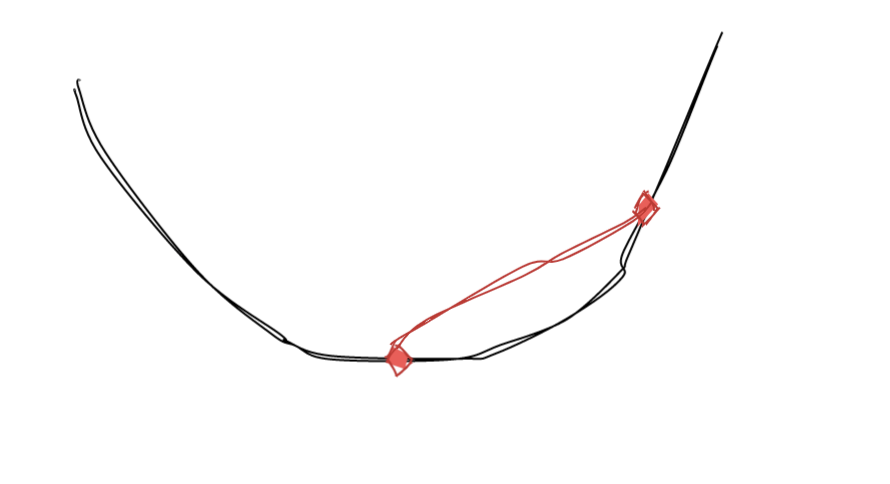
\includegraphics[width=0.5\textwidth]{images/conv.png}
    \caption{Выпуклость означает, что если между любыми двумя точками провести отрезок, функция окажется снизу}
\end{figure}

\underline{Примеры:}
\begin{itemize}
    \item $f(x) = x^2$ -- выпуклая
    \item $f(x) = \exp(x)$ -- выпуклая
    \item $f(x) = \log(x)$ не является выпуклой
\end{itemize}
\bigskip



\textbf{Сильная выпуклость.}

\textbf{Определение.} Функция называется \textit{сильно выпуклой} с параметром $\mu > 0$, если $f(x) - \dfrac{\mu}{2}\|x^2\|$ -- выпуклая.
Также справедливо:

$$f(x) - \dfrac{\mu}{2}\|x^2\|\text{ -- выпуклая} \Leftrightarrow f(y) \geq f(x) + \nabla f(x)^T(y-x) + \dfrac{\mu}{2}\|y-x\|^2\ \ \forall x, y$$

И еще:

$$f\in C^2, f - \mu\text{-сильно выпукла}\ \Leftrightarrow\ \lambda_{\min}(\nabla^2 f(x)) \geq \mu$$

Таким образом, если есть и липшициевость, и сильная выпуклость, максимальное и минимальное собственное значение гессиана ограничено, это круто.

\underline{Примеры:}
\begin{itemize}
    \item $f(x) = x^2$ -- сильно выпуклая с $\mu = 2$
    \item $f(x) = \exp(x)$ -- не является сильно выпуклой, т.к. вторя производная может быть сколь угодно близкой к 0
\end{itemize}

    \subsection{Выпуклые множества и функции. Операции, сохраняющие выпуклость. Простейшие свойства выпуклых функций (неравенство Йенсена, выпуклость надграфика, выпуклость множеств подуровней). Дифференциальные критерии выпуклости. @mercivboku}

    \textbf{Выпуклые множества.}
Пусть $U$ -- вещественное векторное пространство, $Q$ -- подмножество $U$. Множество $Q$ называется \textit{выпуклым}, если для любых двух точке $x,\ y \in Q$ и любого $\lambda \in [0; 1]$ точка $\lambda x + (1 - \lambda) y$ также принадлежит множеству $Q$.

Примеры: Все пространство $U,$ множество из одного элемента, выпуклое множество, множество решений системы линейных неравенств:

\[Q := \{x\in U : \langle a_i, x\rangle \leq b_i \forall i\in I\}.\]

\begin{figure}[H]
    \centering
    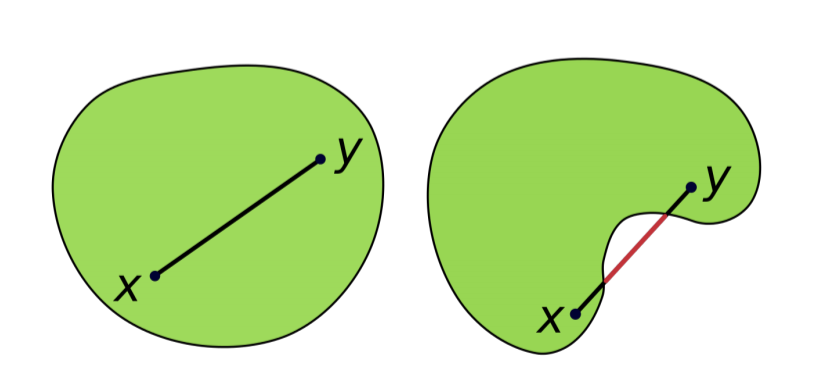
\includegraphics[width=0.5\textwidth]{images/conv_set.png}
    \caption{Слева -- выпуклое, справа -- не выпуклое.}
\end{figure}

\textbf{Свойства выпуклых функций}
\begin{enumerate}
    \item (Неравенство Йенсена) Пусть $U$ -- вещественное векторное пространство, $Q$ -- непустое выпуклое множество в $U$, и $f " Q \to \mathbb{R}$ -- выпуклая функция. Пусть также $x_1,\ldots, x_k$ -- точки в множестве $Q$ и $\lambda_1,\ldots, \lambda_k$ -- неотрицательные коэффициенты, сумммирующиеся в единицу: $\lambda_i \geq 0$ и $\sum_{i = 1}^n \lambda_i = 1.$ Тогда справедливо следующее неравенство:

    $$f\left(\sum\limits_{i= 1}^k \lambda_i x_i\right) \leq \sum_{i = 1}^k \lambda_i f(x_i),$$

    причем равенство достигается тогда и только тогда, когда функция $f$ является афинной или когда все точки совпадают: $x_1 = \ldots = x_k.$

    Другими словами, неравенство Йенсена говорит о том, для выпуклой функции значение функции от выпуклой комбинации точек не превосходит соответствующей выпуклой комбинации значений функции.

    \item(Надграфик) Пусть $U$ -- вещественное векторное пространство, $Q$ -- непустое множество в $U$. \textit{Надграфиком} функции $f : Q \to \mathbb{R}$ называется множество

    $$\mathsf{Epi}(f) := \{(x, t)\in Q \times \mathbb{R}: f(x) \leq t\}. $$
    Надграфик -- это множество из пространства $U \times \mathbb{R}.$

    \begin{figure}[H]
        \centering
        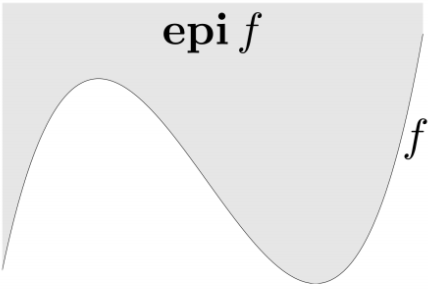
\includegraphics[width=0.5\textwidth]{images/epi.png}
        \caption{Все серое -- надграфик функции $f(x)$.}
    \end{figure}

    \textbf{Определение.} (Выпуклости через надграфик). Пусть $U$ -- вещественное векторное пространство, $Q$ -- непустое выпуклое множество в $U$. Функция $f : Q \to \mathbb{R}$ явдяется выпуклой тогда и только тогда, когда ее надграфик $\mathsf{Epi}(f)$ является выпуклым множеством в пространстве $U\times \mathbb{R}.$
    \bigskip

    \textbf{Утверждение.} (Выпуклость множества линий уровня). Пусть $U$ -- вещественное векторное пространство, $Q$ -- непустое множество в $U$, и пусть $f : Q \to \mathbb{R}$ -- выпуклая функция. Тогда для любого $\alpha \in \mathbb{R}$ соответствующее множество линий уровня

    $$\mathsf{Lev}_f(\alpha) := \{x\in Q: f(x) \leq \alpha\}$$

    является выпуклым.

    \item (Дифференциальные критерии выпуклости).\\
    \textbf{Утверждение.}(Условие выпуклости первого порядка). Пусть $Dom(f)$ является открытым множеством, и функция $f$ дифференцируема всюду на $Dom(f).$ Функция $f$ является выпуклой тогда и только тогда, когда $Dom(f)$ является выпуклым множеством и

    $$f(y) \geq f(x) + \langle\nabla f(x), y - x\rangle$$

    для всех $x,\ y\in Dom(f).$
    \bigskip

    \textbf{Утверждерние.} (Дифференциальное условие оптимальности для выпуклой функции). Пусть $f : U \to \mathbb{R}\sup \{+\infty\}$ -- выпуклая функция, $Dom(f)$ является открытым множеством, и пусть $x^* \in Dom(f).$ Тогда $x^*$ является глобальным минимумом функции $f$, если и только если $\nabla f(x^*) = 0.$ Другими словами, любая стационарная точка автоматически является глобальным минимумом функции $f.$

    \textbf{Утверждение.} (Условие выпуклости второго порядка). Пусть $Dom(f)$ является открытым множеством, и функция $f$ дважды дифференцируема на $Dom(f)$. Функция $f$ является выпуклой тогда и только тогда, когда $Dom(f)$ является выпуклым множеством и

    $$D^2f(x)[h, h] := \langle\nabla^2 f(x) h, h\rangle \geq 0$$

    для всех $x\in Dom(f)$ и всех $h\in U$. Если $U = \mathbb{R}^n,$ то это эквивалентно положительной полуопределенности гессиана:

    $$\nabla^2 f(x) \succcurlyeq 0$$

    для всех $x\in Dom(f).$

\end{enumerate}

    \subsection{Определения субградиента и субдифференциала. Субдифференциальное исчисление (умножение на скаляр, композиция с аффинным преобразованием, теорема Моро–Рокафеллара, максимум конечного числа функций и теорема Данскина). @poly\_nomial}

    Субдифференциал функции: 
$$\partial F(x)=\{z|F(y) \geq F(x) + z^T(y-x)~\forall y\}$$
Фактически это множество касательных к функции в точке $x$. Если функция гладкая и дифференцируемая в каждой точке, то в этом множестве будет всего одна касательная - градиент к функции в каждой её точке. Т.е.
$$
\text{Если}~F(x) \in C^1 \to \partial F(x)=\{\nabla F(x)\}
$$
Если же функция просто гладкая, но производная есть не в каждой её точке - тогда и будет получено данное мн-во.\\
Пример:\\
$$
F(x)=|x| \to \partial F(x)\begin{cases}
x > 0,~\{1\}\\
x < 0,~\{-1\}\\
x = 0.~[-1,1]
\end{cases}
$$
Здесь в качестве $z$ получены коэф-ты к касательным в каждой точке функции. Последний случай также очень легко проверяется:
$$
F(y) \geq F(0) + z^T(y-0)~\forall y \to |y| \geq z*y \to \begin{cases}
1)~y>0 \to z \leq 1\\
2)~y < 0 \to z \geq -1
\end{cases}
$$
Также субдифференциал это выпуклое мн-во, проверяется легко через его определение:
$$
z_1,z_2 \in \partial F(x) \to \begin{cases}
F(y) \geq F(x) + z_1^T(y-x)\\
F(y) \geq F(x) + z_2^T(y-x)
\end{cases}~\forall y \to
$$
$$
\alpha F(y) + (1-\alpha) F(y) \geq \alpha(F(x) + z_1^T(y-x)) + (1-\alpha)(F(x) + z_2^T(y-x)) \to
$$
$$
F(y) \geq F(x) + (\alpha z_1 + (1-\alpha)z_2)^T(y-x) \to \alpha z_1 + (1-\alpha)z_2
$$
Субградиент - эл-т из мн-ва субдифференциала: $z \in \partial F(x)$.\\

    \subsection{Сопряженная функция Фенхеля. Неравенство Фенхеля–Юнга. Теорема Фенхеля–Моро. Связь сопряженной функции с субдифференциалом. @poly\_nomial}

    \textbf{Сопряженная функция Фенхеля}. Пусть $f:~E \to \mathbb{R}$~-~функция, заданная на множестве $E$ в евклидовом пр-ве $V$. Сопряженной функцией для функции $f$ наз-ся функция $f^{*}:~E_{*} \to \mathbb{R}$, определенная как
$$
f^{*}(s):=\underset{x \in E}{sup}\{<s,x>-f(x)\},
$$
где $E_{*}:=\{s \in V:~sup_{x \in E}\{<s,x>-f(x) < +\infty\}\}$. Её и называют сопряж. функцией Фенхеля, а преобразование $f \to f^{*}$ зовут преобр. Фенхеля/Лежандра.\\
Сопряж ф-ия также зависит от скалярного произведения в пр-ве $V$, про него стоит дополнительно пояснять. Везде дальше в курсе по дефолту - стандартное.\\

\textbf{НЕравенство Фенхеля-Юнга}. Пусть $f:~E \to \mathbb{R}$~-~функция, заданная на множестве $E$ в евклидовом пр-ве, и пусть $f^{*}:~E_{*} \to \mathbb{R}$~-~сопряженная функция. Тогда для всех $x \in E$ и всех $s \in E_{*}$~выполнено:
$$
<s,x> \leq g(s) + f(x).
$$
Несмотря на свою простоту, это утв. иметт многочисленные приложения. Нер-во Фенхеля-Юнга дает систематичный способ построения оценок вида
$$
<s,x> \leq f^{*}(s)+f(x),~~~~(1)
$$
для всех $s$ и $x$, где $f$ и $g$~-~некоторые функции. Необходимость сопрженной функции можно связать с таким вопросом: какие пары функций $f,g$ нужно брать в нер-ве $(1)$, чтобы оно было "максимально точным"?. Если зафиксировать конкретным значением функцию $f$, то другая функция $g$, дающая максимальную "точную" оценку в нер-ве $(1)$ уже определяется однозначно - в точности сопряженная функция $f^{*}$.\\
Пример с поиском сопряженной функции: пусть $V$~-~евклидово пр-во, и пусть $f:~V \to \mathbb{R}$~-~функция $f(x):=<a,x>$, где $a \in V$. Поскольку
$$
\underset{x \in V}{sup}\{<s,x>-<a,x>\}=\underset{x \in V}{sup}<s-a,x>=\begin{cases}
0,\text{~если~}s=a,\\
+\infty,\text{~иначе~}
\end{cases}
$$
для всех $s \in V$, то сопряженная функция $f^{*}$~-~это индикаторная функция $\delta_{\{a\}}$ одноэлементного мн-ва $\{a\}$. И пример наоборот:\\

Пусть $V$~-~евклидово пр-во, $a \in V$, и пусть $\delta{\{a\}}:~\{a\} \to \mathbb{R}$~-~индикаторная функция одноэлементного мн-ва $\{a\}$. Поскольку для $s \in V$ выполнено
$$
\underset{x \in \{a\}}{sup}\{<s,x>-\delta_{\{a\}}(x)\}=<s,a>,
$$
то сопряженная функция $\delta^{*}_{\{a\}}$ равна линейной форме $x \to <a,x>$, рассмотренной в предыдущем примере.\\

В след теормине будут несколько примеров, которые показывают, что преобразование Фенхеля это инволюция, т.е. сопряженная функция $f^{**}$ к функции $f^{*}$~-~это исходная функция $f$. На основе этой идеи существует теорема Фенхеля-Моро.\\

\textbf{Теоремка Фенхеля-Моро}. Пусть $f$~-~функция, заданная на непустом множестве в евклидовом пространстве. Тогда $f=f^{**}$, если и только если $f$ является выпуклой и замкнутой.\\

В одну сторону теоремка очевидна: если $f=f^{**}$, то $f$ обязана быть выпуклой и замкнутой, т.к. сопряженная сопряж. функция к любой функции (в том числе к $f^{*}$) является выпуклой и замкнутой вне зависимости от того, обладала ли исходная функция этими свойствами или нет. Нетривиальный частью теоремы Фенхеля-Моро является обратное утв., что замкнутость $f$ является не только необходимым условием, но и достаточным. (хз как доказывать в эту сторону, наверно уточним у Кропотова, надо ли это делать).\\

Список кучи полезных свойств с сопряженными функциями. Пусть $f:~E \to \mathbb{R}$ и $g:~G \to \mathbb{R}$~-~функции, заданные на множествах $E$ и $G$ в евклидовых пр-вах $V$ и $W$ соответственно, и пусть $f^{*}:E_{*} \to \mathbb{R}$ и $g^{*}:~G_{*} \to \mathbb{R}$~-~соответствующие сопряженне функции.\\
\begin{enumerate}
    \item (Умножение на полож. скаляр) Если $c > 0$, то $(cf)^*:~cE_{*} \to \mathbb{R}$~-~это функция $(cf)^*(s)=cf^*(s/c)$ для всех $s \in E_{*}$
    \item (Сдвиг аргумента) Пусть $a \in V$, и пусть $h:~E - a \to \mathbb{R}~-~функция h(x):=f(x+a)$. Тогда $h^*:~E_* \to \mathbb{R}$~-~это функция $h^*(s)[f^*(s)-<s,a>$ для всех $s \in E_*$.
    \item (Прибавление аффинной функции) Пусть $a \in V,~b \in mathbb{R}$ и пусть $h:~E \to \mathbb{R}$~-~функция $h(x):=f(x)+<a,x>+b$. Тогда $h^*:E_*+a \to \mathbb{R}$~-~это функция $h^*(s)=f^*(s-a)-b$ ждя всеъ $s \in E_* + a$.
    \item (Композиция с обратимым лин. преобразованием) Пусть $A:~V \to V$~-~обратимое линейное преобразование. Тогда $(f \circ A)^*:~A^*(E_*) \to \mathbb{R}$~-~это функция $(f \circ A)*(s)=f^*(A^{-*}s)$ для всех $s \in A^*(E_*)$.
    \item (Сепарабельная сумма). Пусть $\phi:E \times G \to \mathbb{R}$~-~функция $\phi(x,y):=f(x)+g(y)$. Тогда $\phi^*:E_* \times G_* \to \mathbb{R}$~-~это функция $\phi_*(s,u)=f^*(s)+g^*(u)$ для всеъ $s \in E_*$ и всех $u \in G_*$.
\end{enumerate}

На применение этих исчислений могут спокойно дать задачу какую-нибудь.\\

Перед выводом связи меж сопряж ф-ей и субдифф-ом стоит рассмотреть след пример. Пусть $V$~-~конечномерное евклидово пр-во, $x_0 \in V$. Пусть $||~||$~-~произвольная норма в $V$ (необязательно индуцированная скалярным произведением), и $||~||_{*}$~-~соотв. сопряженная норма. Тогда:
$$
\partial||~||(x_0) = \{s \in V:||s||_{*} \leq 1; <s,x_0>=||x_0||\}=\begin{cases}
\overline{B_{||~||}},(0,1),\text{если}~x_0=0\\
{s \in V: ||s||_{*}=1;~<s,x_0>=||x_0||}, \text{иначе}
\end{cases}~~~~(1)
$$
Где $\overline{B_{||~||}},(0,1):=\{s \in V:||s||_{*} \leq 1\}$~-~замкнутый единичный шар с центром в нуле относительно сопряженной нормы. Другими словами, вектор $s \in V, ||s||_{*}=1$, является субградиентом нормы $||~||$ в точке $x_0 \neq 0$, если и только если нер-во Гельдера (след пункт теормина)~$<s,x_0> \leq ||x_0||$~переходит в равенство.\\

\textit{Док-во}. Пусть $s \in V$. По опр субградиента: $s \in \partial ||~||(x_0)$, если и только если $$
<s,x>-||x|| \leq <s,x_0>-||x_0||
$$
,для всех $x \in V$, или, квивалентно
$$
\underset{x \in V}{sup}\{<s,x>-||x||\} \leq <s,x_0>-||x_0||.~~~(*)
$$
По определению супремума, последнее равносильно(тут даже автор конспекта чет сомневается)
$$
\underset{x \in V}{sup}\{<s,x>-||x||\}=<s,x_0>-||x_0||
$$
Заметим, что выражение в левой части есть супремум из опредеелния сопряженной функции Фенхеля для нормы, который, как мы уже знаем, равен:
$$
\underset{x \in V}{sup}\{<s,x>-||x||\}=\begin{cases}
0, \text{если} ||s||_{*} \leq 1,\\
+\infty, \text{иначе}
\end{cases}
$$
Таким образом, $(*)$~эквивалентно
$$
||s||_{*} \leq 1~~\text{и}~~<s,x_0>=||x_0||.
$$
В итоге
$$
\partial||~||(x_0)=\{s \in V:||s||_{*}\leq 1; <s,x_0>=||x_0||\}.
$$
Остается заметить, что для $x_0 \neq 0$~нер-во $||s||_{*} \leq 1$~обязано переходить в равенство, поскольку при $||s||_{*} < 1$, из нер-ва Гельдера следует $<s,x_0> \leq ||s||_{*}||x_0|| < ||x_0||$. (одним словом - ужас).\\
На этом примере с сопряженной нормой можно понять, что аналогичным образом для произвольной функции $f$ (т.е. не только для нормы) ее субдиф можно описать в терминах двойственного объекта - сопряженной функции Фенхеля.\\

Тогда в сухом остатке эта формулировка звучит так: Пусть $f: E \to \mathbb{R}$~-~функция, определенная на мн-ве $E$ в евклидовом пр-ве. Пусть $x_0 \in E$, и пусть $f^*:E \to \mathbb{R}$~-~сопряженная функция. Тогда можно показать, что
$$
\partial f(x_0)=\{s \in E_{*}:<s,x_0>=f^{*}(s)+f(x_0)\}~~~(2)
$$
Словами: вектор $s \in E_{*}$~является субградиентом функции $f$ в точке $x_0$, если и только если неравенство Фенхеля-Юнга $<s,x_0> \leq f^{*}(s)+f(x_0)$~переходит в равенство.\\
В случае $f=||~||$, получаем $f^{*}=\delta_{\overline{B_{||~||}},(0,1)}$, т.е. сопряженная функция равна индикаторной функции шара $\overline{B_{||~||}},(0,1)$ и формула выше~$(2)$~переходит в формулу из примера~$(1)$~.\\

Следствие из этих рассуждений - критерии равенства в нер-ве Фенхеля-Юнга. Пусть $f:~R \to \mathbb{R}$~-~выпуклая замкнутая функция, $f^{*}:E_{*} \to \mathbb{R}$~-~сопряженная функция, и пусть $x \in E,~s \in E_{*}$. Тогда след. утверждения эквивалентны:\\
1. $<s,x>~=~f^{*}(s)+f(x)$\\
2. $s \in \partial f(x)$.\\
3. $x \in \partial f^{*}(s)$.\\
\textit{Док-во}. Согласно выводу по связи сопряж функции и субдиф-ов, условие $<s,x>=f^{*}(s)+f(x)$~равносильно вложению $s \in \partial f(x)$. С другой стороны, поскольку $f$ выпуклая и замкнутая, то, по теореме Фенхеля-Моро, $f^{**}=f$. Применяя вывод по связи выше к функции $f^{*}$, получаем, что равенство $<s,x>=f^{*}(s)+f(x)$~эквивалентно вложению $x \in \partial f^{*}(s)$.

Открытый вопрос: надо ли в рамках этого пункта что-то про двойственность фенхеля говорить. Ответ узнаем завтра на консе.

    \subsection{Сопряженная норма. Неравенство Гельдера. Основные примеры. @poly\_nomial}

    \textbf{Сопряженная норма}. Пусть $V$~-~конечномерное евклидово пр-во, пусть $||~||$~-~произвольная норма в $V$ (необяхательно индуцированная скалярным произведением). Тогда \textit{сопряженной нормой} для $||~||$ называется норма $||~||_*$, опредленная как
$$
||s||_*:=\underset{||v||=1}{max}|<s,v>|.
$$
Заметим, что это определение корректное, поскольку максимум достигается по теореме Вейерштрасса в силу компактности единичной сферы.\\
Теперь примеры по работе с этой нормой:\\

Пусть $p \in [1,+\infty]$, и пусть $||~||_p:~\mathbb{R}^n \to \mathbb{R}$~-~$l^p$-норма. Тогда из нер-ва Гельдера следует, что сопряженная норма $(||~||_p)_*$~-~это $l^q$-норма $||~||_q$, где $q \in [1, +\infty]$ определяется из неравенства $1/p$ + $1/q=1$. В частности $l^1$~-~норма является сопряженной к $l^{\infty}$~-~норме; в то же время, $l^{\infty}$~-~норма является сопряженной к $l^1$~-~норме, а $l^2$ норма является самосопряженной.

Беда.(около консы тут будут нужные примеры и нормальный вариант нер-ва гельдера).

    \subsection{Проксимальный оператор. Связь с евклидовой проекцией. @bigbluebutterfly}

    Пусть $f: E \to \mathbb{R}$  - функция, заданная на множестве $E$ в евклидовом пространстве $V$. Определим проксимальный оператор функции $f$ как отображение $\text{Prox}_f : V \to E$, заданное следующим образом: $$ \text{Prox}_f(x) := \arg\min\limits_{y \in E} \left\{f(y) + \frac{1}{2} ||y-x||^2 \right \}$$ Если функция $f$ выпуклая и замкнутая, то в каждой точке множество значений $\text{Prox}_f$ состоит из одного элемента как множество минимумов сильно выпуклой и замкнутой функции. 

Рассмотрим функцию $g: E \to \mathbb{R}$, определенную как $$g(x) = \delta_C (x)$$ т.е. $g$ - индикаторная функция непустого множества $C \subseteq E$. Запишем проксимальное отображение для данной функции: $$\text{Prox}_g(x) = \arg\min\limits_{y \in E} \left\{ \delta_C(y) + \frac{1}{2}||y-x||^2 \right\} = \arg\min\limits_{y \in C} ||y-x||^2 = P_C(x)$$   Таким образом, проксимальный оператор для индикаторной функции данного множества есть оператор ортогональной проекции на данное множество. Если $C$ - замкнутое и выпуклое (а также непустое), то проецирующее отображение существует и единственно в каждой точке.


    \subsection{Основные матричные разложения, их стоимость вычисления. @bigbluebutterfly}

    $LU$-разложение матрицы $A$:
$$ A = LU$$где $L$ - нижнетреугольная матрица, $U$ - верхнетреугольная матрица. Собственно, разложение определено только для обратимых матриц с невырожденными главными минорами. В общем случае разложение определено неоднозначно - для однозначности можем потребовать унитреугольность матрицы $L$ или $U$. Используется для нахождения определителя, решения СЛАУ и обращения матриц. Сложность $\approx \frac{2}{3} n^3$.

Разложение Холецкого:
$$ A = LL^T$$ $A$ - симметричная положительно определенная матрица, $L$ - нижнетреугольная матрица (можно также записать как $U^T U$ через верхнетреугольную матрицу). Данное разложение единственно для любой удовлетворяющей условиям матрицы. Применяется для решения СЛАУ - в отличие от $LU$, здесь требуется примерно в 2 раза меньше итераций ($\frac{1}{3}n^3$) , при этом имеет место большая численная устойчивость. Часто применяется для решения задачи наименьших квадратов. Также используется в квази-ньютоновских методах.

Разложение можно немного модифицировать: $$A = LDL^T$$$D$ - диагональная матрица, диагональ которой является квадратом диагонали матрицы $L$ в исходном разложении - соответственно, у матрицы $L$ теперь будет единичная диагональ. С таким методом мы избавляемся от вычисления корней диагональных элементов в процессе факторизации. Кроме того, для некоторых неопределенных матриц существует $LDL$-разложение (в отличие от разложения Холецкого). Сложность сохраняется.

$QR$-разложение: $$ A = QR$$ где $Q$ - унитарная матрица ($Q^T Q = QQ^T = E$), $R$ - верхнетреугольная матрица. Разложение существует для любой матрицы (более того, существует даже для прямоугольной размера $m \times n$  ($m > n$) - тогда получаем $Q$ размера $m \times m$ и верхнетреугольную $R$ размера $m \times n$). Разложение чаще всего применяется для решения задачи наименьших квадратов, также используется в одном из алгоритмов для поиска собственных чисел и векторов. Стоимость вычисления $\approx \frac{2}{3}n^3$.

Сингулярное разложение:
$$ M = U \Sigma V^T$$ где $M$ - произвольная матрица размера $m \times n$, $\Sigma$ - диагональная матрица размера $m \times n$, составленная из сингулярных чисел $M$, матрицы $U$ ($m \times m$) и $V$ ($n \times n$) являются унитарными и составлены из левых и правых сингулярных векторов соответственно. Применяется для нахождения псевдообратной матрицы (используется в МНК) или низкоранговых приближений. Сложность - $O(m^2n + mn^2 + n^3)$, в квадратном случае справедлива оценка $4n^3$.


Спектральное разложение:
$$A = V \Lambda V^{-1}$$
где $A$ - диагонализуемая квадратная матрица размера $n \times n$, имеющая $n$ линейно независимых собственных векторов, $V$ - матрица из собственных векторов-столбцов для $A$, $\Lambda$ - диагональная матрица с соответствующими собственными числами на диагонали. Разложение можно использовать для обращения матриц, решения СЛАУ, нахождения определителя и вычисления функций от матриц (к примеру, матричная экспонента). Сложность $\approx O(n^3)$. 


    \subsection{Формулировка теоремы Каруша-Куна-Таккера для общей задачи нелинейного программирования. @Bitchert}

    Задача оптимизации:
\[
    \begin{cases}
        \label{kkt}
        f(x) \to \min\limits_{x \in D \subset \mathbb{R}^{n}}, \\
        g_{i}(x) \leq 0, \quad i \in \{ 1, \dots , m \}, \\
        h_{j}(x) = 0, \quad j \in \{ 1, \dots , p \}.
    \end{cases}
\]
Доменное множество (совместная область определения, где определены все функции):
\[
    D = \dom f \bigcap \left( \capl\limits_{i=1}^{m} \dom g_{i} \right) \bigcap \left( \capl\limits_{j=1}^{p} \dom h_{j} \right)
\]
Допустимое множество (все точки из доменного множества, которые удовлетворяют ограничениям $g$ и $h$):
\[
    F = \left\{ x \in D \,|\, g_{i}(x) \leq 0 \, \forall i,\,\, h_{j}(x) = 0 \, \forall j \right\}
\]
Активное множество (множество ограничений, все ограничения которые имеют вид равенства в точке):
\[
    \text{Active} (x) = \{ 1, \dots , p \} \cup \{ i \,|\, g_{i}(x) = 0 \}
\]
Функция Лагранжа:
\[
    L(x, \lambda, \mu) = f(x) + \sum\limits_{i=1}^{m} \lambda_{i} g_{i}(x) + \sum\limits_{j=1}^{p} \mu_{j} h_{j}(x)
\]
Условия регулярности:
\begin{itemize}
    \item \textbf{LCQ} все функции $g_{i}, h_{j}$ являются невырожденными афинными
    \item \textbf{LICQ} вектора $\nabla g_{i}(x), \nabla h_{j}(x)$ для $i, j \in \text{Active}(x)$ являются линейно независимыми
    \item \textbf{MFCQ} вектора $\nabla g_{i}(x), \nabla h_{j}(x)$ для $i, j \in \text{Active}(x)$ являются линейно независимыми с положительными коэффициентами
    \item \textbf{условия Слейтера} для выпуклых задач оптимизации найдется $\widetilde{x}$ такое, что $h_{j}(\widetilde{x}) = 0 \, \forall j$ и $g_{i}(\widetilde{x}) < 0 \, \forall i$
    \item \textbf{ослабленные условия Слейтера} для выпуклых задач оптимизации найдется $\widetilde{x}$ такое, что $h_{j}(\widetilde{x}) = 0 \, \forall j$ и $g_{i}(\widetilde{x}) \leq 0$ для всех аффинных функций $g_{i}$ и $g_{i}(\widetilde{x}) < 0$ для остальных
\end{itemize}
Теорема ККТ:
\theorem{
Пусть в \hyperref[kkt]{задаче оптимизации} $f, g_{i}, h_{j} \in C^{1}$, $x_{*}$ - точка локального экстремума и выполнены условия регулярности для $\{ g_{i}(x_{*}),\, h_{j}(x_{*}) \,|\, i, j \in \text{Active}(x_{*}) \}$. \\ Тогда найдутся $\lambda_{*}, \mu_{*}$ такие, что:
\begin{itemize}
    \item $\nabla_{x}L(x_{*}, \lambda_{*}, \mu_{*}) = \nabla f(x_{*}) + \sum\limits_{i=1}^{m} \lambda_{i} \nabla g_{*, i}(x_{*}) + \sum\limits_{j=1}^{p} \mu_{*, j} \nabla h_{j}(x_{*}) = 0$ - станционарность функции Лагранжа.
    \item $x_{*} \in F$ - прямая допустимость
    \item $\lambda_{*, i} \geq 0 \, \forall i$ - двойственная допустимость
    \item $\lambda_{*, i} g_{i}(x_{*}) = 0 \, \forall i$ - условия дополняющей нежесткости
\end{itemize}
}
Она утверждает, что для задач для которых справедливо некоторое условие регулярности, если точка $x_{*}$ — локальный минимум, то мы можем выписать уравнения стационарности и дополняющей нежёсткости которые обязательно разрешимы с некоторыми, неизвестными нам двойственными переменными. \\ \\
\textit{Опциональный материал:} \\ \\
Введем два множества - $\mathcal{S}(x_{0})$ множество всех гладких траекторий выходящих из $x_{0}$ и остающихся в множестве $F$; $\mathcal{T}_{F}(x_{0})$ касательное пространство к множеству $F$ в точке $x_{0}$:
\begin{gather*}
    \mathcal{S}(x_{0}) = \left\{ x(t) \,|\, x(t) \in F \, \forall t \geq 0; x(0) = x_{0}; x(t) \in C^{1} \right\}\\
    \mathcal{T}_{F}(x_{0}) = \left\{ d \,|\, \exists x(t) \in \mathcal{S}(x_{0}),\, \left. d = \dfrac{\partial x}{\partial t}\right|_{t = 0} \right\}\\
\end{gather*}
Теорема ККТ второго порядка:
\theorem{
Пусть в \hyperref[kkt]{задаче оптимизации} $f, g_{i}, h_{j} \in C^{2}$, $x_{*}$ - точка локального минимума и выполнены условия регулярности для $\{ g_{i}(x_{*}),\, h_{j}(x_{*}) \,|\, i, j \in \text{Active}(x_{*}) \}$. \\ Тогда найдутся $\lambda_{*}, \mu_{*}$ такие, что:
\begin{itemize}
    \item $\nabla_{x}L(x_{*}, \lambda_{*}, \mu_{*}) = \nabla f(x_{*}) + \sum\limits_{i=1}^{m} \lambda_{i} \nabla g_{*, i}(x_{*}) + \sum\limits_{j=1}^{p} \mu_{*, j} \nabla h_{j}(x_{*}) = 0$ - станционарность функции Лагранжа.
    \item $x_{*} \in F$ - прямая допустимость
    \item $\lambda_{*, i} \geq 0 \, \forall i$ - двойственная допустимость
    \item $\lambda_{*, i} g_{i}(x_{*}) = 0 \, \forall i$ - условия дополняющей нежесткости
    \item $d^{T} \nabla^{2}_{xx} L(x_{*}, \lambda_{*}, \mu_{*})d \geq 0 \, \forall d \in \mathcal{T}_{F}(x_{*})$
\end{itemize}
}
Если выполнены условия регулярности, то можно записать $\mathcal{T}_{F}(x_{0})$ в виде:
\[
    \mathcal{T}_{F}(x_{0}) = \left\{ d \,|\, \nabla g_{i}(x_{0})^T d \leq 0, \, \nabla h_{j}(x_{0})^T d \leq 0 \, \forall i, j \in \text{Active}(x_{0}) \right\}
\]

    \subsection{Каноническая форма задачи линейного программирования. Пример сведения общей задачи ЛП к задаче в канонической форме. @Bitchert}

    Задача линейного программирования в общем виде:
\[
    \begin{cases}
        c^{T} x \to \min\limits_{x} \\
        Ax = b \\
        Ex \leq d
    \end{cases}
\]
Задача линейного программирования в \textbf{канонической форме}:
\[
    \begin{cases}
        c^{T} x \to \min\limits_{x \in \mathbb{R}^{n}} \\
        Ax = b, \quad A \in \mathbb{R}^{p \times n}, p < n, \Rk(A) = p \\
        x \geq 0
    \end{cases}
\]
Эквивалентные преобразования для сведения задачи к канонической форме:
\begin{itemize}
    \item $Ex \leq d \Leftrightarrow \begin{cases}
                                         Ex + f = d \\ f \geq 0
    \end{cases}$
    \item $Ax = b \Leftrightarrow \begin{cases}
                                      A(x^{+} - x^{-}) = b \\ x = x^{+} - x^{-}, \quad x^{+} = \max(x, 0), \quad x^{-} = \max(-x, 0) \\ x^{+}, x^{-} \geq 0
    \end{cases}$
\end{itemize}
Пример сведения:
\[
    \begin{cases}
        c^{T} x \to \min\limits_{x} \\
        Ax = b \\
        Ex \leq d
    \end{cases}
    \Leftrightarrow
    \begin{cases}
        c^{T} (x^{+} - x^{-}) \to \min\limits_{x^{+}, x^{-}} \\
        A(x^{+} - x^{-}) = b \\
        E(x^{+} - x^{-}) + f = d \\
        x^{+}, x^{-}, f \geq 0
    \end{cases}
\]

    \subsection{Двойственная задача Лагранжа и ее основные свойства. Пример построения двойственной задачи. @Bitchert}

    Задача условной оптимизации:
\[
    (P)
    \begin{cases}
        f(x) \to \min\limits_{x} \\
        g_{i}(x) \leq 0, \, i \in \{ 1, \dots , m \} \\
        h_{i}(x) = 0, \, j \in \{ 1, \dots , p \} \\
    \end{cases}
    \quad f, g_{i}, h_{j} \in C^{1}
\]
Функция Лагранжа:
\[
    L(x, \lambda, \mu) = f(x) + \sum\limits_{i=1}^{m} \lambda_{i} g_{i}(x) + \sum\limits_{j=1}^{p} \mu_{j} h_{j}(x)
\]
Двойственная функция Лагранжа:
\[
    q(\lambda, \mu) := \inf\limits_{x} L(x, \lambda, \mu)
\]
Свойства двойственной функции:
\begin{itemize}
    \item $q$ - вогнутая функция
    \item $q(\lambda, \mu) \leq f_{opt}$, для $\lambda \geq 0, \mu$
\end{itemize}
Двойственная задача оптимизации:
\[
    (D)
    \begin{cases}
        q(\lambda, \mu) \to \max\limits_{\lambda, \mu} \\
        \lambda \geq 0
    \end{cases}
\]
Двойственность:
\begin{itemize}
    \item \textbf{Слабая} двойственность: $q_{opt} \leq f_{opt}$
    \item \textbf{Сильная} двойственность: $q_{opt} = f_{opt}$
\end{itemize}
Если выполнено условие регулярности и $(P)$ является выпуклой задачей оптимизации, то выполняется сильная двойственность.
Пример построения двойственной задачи: \\
Исходная задача:
\[
    \begin{cases}
        c^{T} x \to \min\limits_{x \in \mathbb{R}^{n}} \\
        Ax \leq b, \quad A \in \mathbb{R}^{m \times n}, \Rk(A) = \min(m, n)
    \end{cases}
\]
Лагранжиан:
\[
    L(x, \lambda) = c^{T} x + \lambda^{T} (Ax - b) = (c + A^{T}\lambda)^{T} x - \lambda^{T} b
\]
Двойственная функция:
\[
    q(\lambda) = \inf\limits_{x \in \mathbb{R}^{n}} L(x, \lambda)
\]
Двойственная задача:
\begin{itemize}
    \item $c + A^{T}\lambda = 0$: \quad $\begin{cases}
                                             q(\lambda) = -\lambda^{T}b \to \max\limits_{y \in \mathbb{R}^{m}} \\ c + A^{T}\lambda = 0 \\ \lambda \geq 0
    \end{cases}$
    \item $c + A^{T}\lambda \neq 0$: $q(\lambda) = -\infty$
\end{itemize}

    \subsection{Общая схема какого-то метода оптимизации (итерация, выбор длины шага, критерий останова), например, градиентного спуска, проксимального градиентного метода, метода SAG, метода логарифмических барьеров и проч.}

    Прежде всего возникает вопрос: а зачем вообще нам нужны нетрадиционные методы оптимизации, раз мы уже разобрали градиентные спуски на любой вкус и цвет, методы Ньютона и прочая, и прочая, и прочая? Дело в том, что разобранные нами методы для условной оптимизации подходят не для всех множеств (например, мы можем захотеть оптимизировать функцию $f(x)$ по шару $x^T x = 1$, а метод барьеров не умеет работать с множествами без внутренности).

Рассмотрим еще один простой пример. Частая проблема в рекуррентных сетях - затухание градиента (когда норма весов $\|W\| < 1$) или взрыв градиента (соответствено, $\|W\| > 1$). Хорошей практикой здесь считается брать матрицу весов $W$ ортогональной, что позволяет контролировать ее норму (она становится единичной). Прелесть римановской оптимизации в том, что она позволяет оптимизировать функции по очень сложным множествам (типа множества ортогональных матриц или шара без внутренности).

Центральным понятием в римановской оптимизации явлется риманов градиент. Рассмотрим ради простоты всю конструкцию на сфере $S^{n-1}$. Рассмотрим некоторую точку сферы $x$ и ее окрестность. \textbf{Римановым градиентом} $\grad f(x)$ называется направление кривой наибольшего возрастания в окрестности точки $x$. Он представляет собой вектор, лежащий в касательной плоскости к сфере в точке $x$.

Казалось бы все, наши проблемы решены! Берем и делаем шаг вдоль направления риманова антиградиента. Но есть проблема: такой шаг выведет нас за пределы нашего множества:

$$
x_{k+1} = x_k - \alpha_k \grad f(x_k) \not\in S^{n-1}
$$

\noindent
Нам нужно как-то шагнуть в сторону уменьшения функции, но при этом остаться на сфере. Для этого вводится операция \textbf{ретракции} - это в некотором смысле проецирование риманова градиента на наше множества. По итогу, чтобы задать риманов градиентный спуск (RGD), нам нужно определить риманов градиент и операцию ретракцию.

$$
x_{k+1} = R_{x_k}\big(-\alpha_k \grad f(x_k)\big)
$$

\begin{figure}[H]
    \centering
    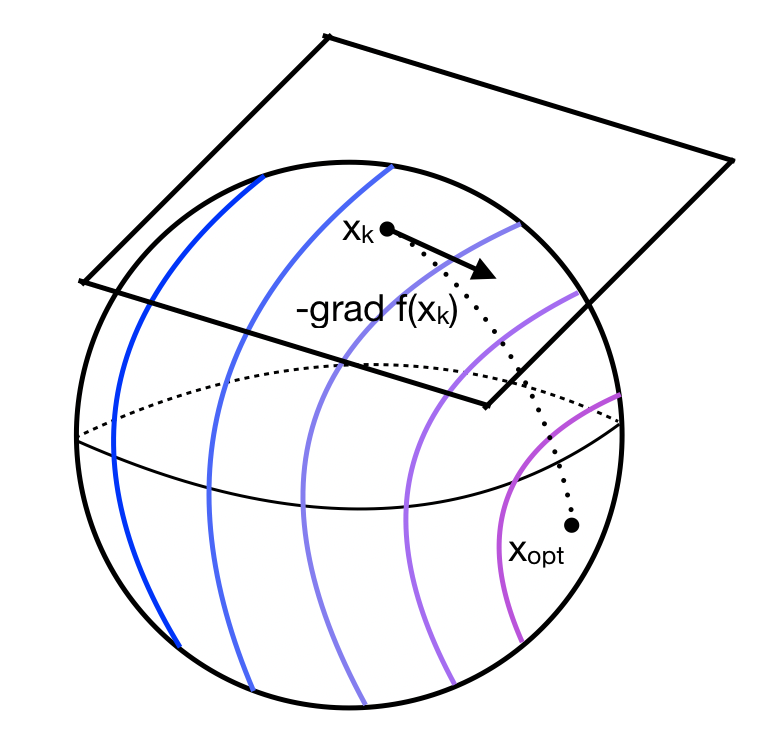
\includegraphics[width=8cm]{images/2-14-sphere.png}
    \caption{Риманов антиградиент в точке $x_k$. Цветными кривыми показаны линии уровня функции $f(x)$.}
    \label{fig:my_label}
\end{figure}

Теперь перейдем к формализму (наверное, правильнее начинать рассказывать билет отсюда, а все, что выше, приведено для понимания общей логики происходящего).

\textbf{Многообразием} $M$ размерности $d$ называется множество, удовлетворяющее двум свойствам:

\begin{enumerate}
    \item $\forall x \in M, U$ - открестность $x$ $\exists$ отображение $\phi: U \rightarrow \R^d$, биективно переводящее $U$ в некоторое открытое множество. Пара $(U, \phi)$ называется картой множества $M$.
    \item Для карт $(U, \phi), (W, \psi)$ в точке $x: U \cap W \ne \O$ отображения $\phi \circ \psi^{-1}$ и $\psi \circ \phi^{-1}$ дифференцируемы бесконечное число раз как функции $\R^d \rightarrow \R^d$.
\end{enumerate}

При этом $\phi(x) \in \R^d$ называются локальными координатами, а если $M \subset \R^n$, то $x \in \R^n$ называются глобальными координатами.

\underline{Примеры многообразий}:

\begin{enumerate}
    \item Окружность $S^1 = \{(x_1, x_2): x_1^2 + x_2^2 = 1\}$. Тогда $t \in [0, 2\pi)$ - это локальные координаты, а в качестве отображения $\phi(x)$ можно взять подходящую обратную тригонометрическую функцию.
    \item Все пространство $\R^n$. В качестве биекции берем тривиальную, а локальные координаты совпадают с глобальными.
    \item Манифолд Штифеля $\text{St}(m, n) = \{X \in \R^{n \times m} \big| X^T X = I_m\}$ (в сущности, множество ортогональных матриц).
\end{enumerate}

\textbf{Касательным пространством} в точке $x \in M$ называется множество $T_x M = \{\xi \in \R^n \big| \xi = \gamma'(0), \text{ где } \gamma(t) - \text{ это кривая в } M \text{ и } \gamma(0) = x\}$. По сути, это множество всех направлений кривых на $M$ в точке $x$.

Для примера найдем касательное пространство для шара $S^{n-1} = \{x \in \R^n \big| x^T x = 1\}$ в точке $x_0$. Интересующее нас множество кривых выглядит так:

$$
\begin{cases}
    x(t)^T x(t) = 1 \\
    x(0) = x_0
\end{cases}
$$

\noindent
Продифференцируем первое уравнение по $t$ и подставим $t=0$:

$$
x'(0)^T x(0) + x(0)^T x'(0) = 0 \Rightarrow x'(0)^T x_0 = 0
$$

\noindent
Обозначим $U_{x_0} = \{z | z^T x_0 = 0\}$. Мы только что доказали, что $T_{x_0} S^{n-1} \subseteq U_{x_0}$. Осталось показать обратное вложение. Пусть $x(t) = \frac{x_0 + tz}{\|x_0 + tz\|}$. Утверждение $x(0) = x_0$ тривиально. Нужно проверить, что $x'(0) = z$:

$$
x^i(t) = \frac{x_0^i + tz^i}{\|x_0 + tz\|}
$$

$$
x^i(t)' = \frac{z^i \|x_0 + tz\| - (x_0^i + tz^i) \frac{2\sum_{j=1}^n (x_0^j + t z^j)z^j}{2\|x_0 + tz\|}}{\|x_0 + tz\|^2} = z^i \frac{1}{\|x_0 + tz\|} - (x_0^i + tz^i) \frac{z^T (x_0 + tz)}{\|x_0 + tz\|^3}
$$

$$
x^i(0)' = z^i - x_0^i z^T x_0 = z^i
$$

\noindent
Таким образом, $x'(0) = z$, а значит, $U_{x_0} \subseteq T_{x_0} S^{n-1}$, и поэтому $T_{x_0} S^{n-1} = U_{x_0}$. Мы получили, что касательное простанство к шару - это множество векторов, перпендикулярных радиусу, что логично. Тут нужно сделать еще два важных замечания:

\begin{enumerate}
    \item $T_x M$ - линейное подпространство
    \item $\Dim T_x M = \Dim M$
\end{enumerate}

Теперь мы готовы ввести центральное понятие. \textbf{Римановым многообразием} называется многообразие $M$, снабженное скалярным произведением на каждом касательном пространстве $T_x M$, его принято обозначать $g_x(\cdot, \cdot) = \langle \cdot, \cdot \rangle_x$. Если $M \subset \R^n$, то в качестве скалярного произведение удобно брать стандартное евклидово.

\textbf{Производной по направлению} $\xi$ в римановском случае называется
$$
D f(x) [\xi] = \frac{df(\gamma(t))}{dt} \bigg|_{t = 0}, \text{ где } \gamma(t) - \text{ кривая в } M: \gamma(0) = x, \gamma'(0) = \xi
$$

\textbf{Римановым градиентом} называется вектор $\grad f(x)$, для которого верно следующее:

$$
\big\langle \grad f(x), \xi \big\rangle_x = D f(x) [\xi], \forall \xi \in T_x M
$$

\noindent
Для градиента верно соображение про максимальное направление роста функции на множестве. В частности, верно следующее (здесь нормы берутся по скалярному произведению из определения риманова многообразия):

$$
\frac{\grad f(x)}{\|\grad f(x)\|} = \argmax_{\xi \in T_x M: \|\xi\| = 1} D f(x) [\xi]
$$

\noindent
При этом, если $M \subset \R^n$, то $\grad f(x) = P_{T_x M} (\nabla f(x))$. Поскольку $T_x M$ - линейное подпространство в $\R^n$, то можно написать $\nabla f(x) = P_{T_x M} (\nabla f(x)) + P_{{T_x M}^\bot} (\nabla f(x))$. Тогда:

$$
\big\langle P_{T_x M} (\nabla f(x)), \xi \big\rangle_x = \Big\langle \nabla f(x) - P_{{T_x M}^\bot} (\nabla f(x)), \xi \Big\rangle_x = \big\{\xi \in T_x M\big\} = \big\langle \nabla f(x), \xi \big\rangle_x = D f(x) [\xi]
$$

\noindent
В последнем равенстве мы получили производную по направлению в евклидовом смысле, но поскольку $\xi \in T_x M$, то она совпадает с римановской. Отсюда $\grad f(x) = P_{T_x M} (\nabla f(x))$.

Обозначим $TM = \bigcup_{x \in M} (x, T_x M)$. \textbf{Ретракцией} называется отображение $R: TM \rightarrow M$ ($R_x: T_x M \rightarrow M$), удовлетворяющее двум свойствам:

\begin{enumerate}
    \item $R_x(0) = x$
    \item $\displaystyle\frac{dR_x(t\xi)}{dt} = \xi, \forall \xi \in T_x M$
\end{enumerate}

\underline{Пример}:
\begin{enumerate}
    \item $S^{n-1}$: $R_x(\xi) = \frac{x + \xi}{\|x + \xi\|}$ (доказательство полностью аналогично примеру про касательное пространство).
    \item $\text{St}(m, n)$: $R_X(\Xi) = (X + \Xi) (I_m + \Xi^T \Xi)^{-1/2}$
\end{enumerate}

\noindent
В общем случае поиск ретракции - это очень нетривиальная задача. В частоности, ретракция определена не единственным образом. Периодически выходят статьи с предложениями разных операторов ретракции.

Теперь мы можем с чистой совестью определить RGD: $x_{k+1} = R_{x_k} (-\alpha_k \grad f(x_k))$. Но мы пойдем дальше и выпишем формулы для RGD с моментумом. Получается система:

$$
\begin{cases}
    d_{k+1} = \beta d_k + \alpha_k \grad f(x_k) \\
    x_{k+1} = R_{x_k} (-d_{k+1})
\end{cases}
$$

\noindent
Видите проблему? Нет? А она есть. Дело в том, что векторы $d_k$ и $\grad f(x_k)$ лежат в разных касательных пространствах ($d_k \in T_{x_{k-1}} M, \grad f(x_k) \in T_{x_k} M$), потому складывать их некорректно. Чтобы избежать этой проблемы, вводится операция транспортировки векторов. \textbf{Транспортировкой} вектора $\xi$ вдоль вектора $\eta$ ($\xi, \eta \in T_x M$) называется отображение $\Transp: TM \times TM \rightarrow TM$, обладающее следующими свойствами:

\begin{enumerate}
    \item $\exists R_x: \Transp_\eta (\xi) \in T_{R_x(\eta)} M$
    \item $\Transp_0 (\xi) = \xi$
    \item $\Transp_\eta (a \xi + b \zeta) = a\Transp_\eta (\xi) + b\Transp_\eta (\zeta)$
\end{enumerate}

Теперь более понятно о том, что только что произошло. Пусть у нас есть векторы $\xi$ и $\eta$ из касательного пространства точки $x$. Мы хотим сместиться из точки $x$ в точку $R_x (\eta)$, но при этом ''забрать с собой'' вектор $\xi$, чтобы он из старого касательного пространства перешел в новое. Для этого и нужна операция транспортировки. Как правило, сначала фиксируют ретракцию, а транспортировку по ней строят так:

$$
\Transp_\eta (\xi) = \frac{d}{dt} R_x (\eta + t\xi) \Big|_{t=0}
$$

\noindent
Для шара $S^{n-1}$ и ретракции $R_x (\xi) = \frac{x + \xi}{\|x + \xi\|}$ транспортировка выглядит так:

$$
\Transp_\eta (\xi) = \frac{1}{\|x+\eta\|} \Big(I_n - \frac{(x+\eta)(x+\eta)^T}{\|x+\eta\|^2} \Big) \xi
$$

Теперь мы можем написать правильные формулы для RGD+momentum. Они выглядят так:

$$
\begin{cases}
    d_{k+1} = \Transp_{-d_k} \big( \beta d_k \big) + \alpha_k \grad f(x_k) \\
    x_{k+1} = R_{x_k} (-d_{k+1})
\end{cases}
$$

\noindent
Стоит отметить, что для римановской оптимизации существуют и алгоритмы линейного поиска, и методы второго порядка, но \textbf{к счастью}, это выходит за пределы нашего курса.


    \newpage

    \section{Билеты}
    \subsection{Матрично-векторное дифференцирование в терминах дифференциалов. Примеры вычисления градиентов и гессианов для матричных функций.}

    Все написано \href{https://drive.google.com/file/d/1bNWF262guJHTphptCTYARAsUKRPC9QmS/view?usp=sharing}{здесь}.

    \subsection{Решение задачи одномерной оптимизации (метод золотого сечения, парабол, Брента). Условия для неточной одномерной оптимизации. @sofloud}

    Рассмотрим задачу одномерной оптимизации вида
\begin{equation}
    \label{formula221}
    f(x)\to \min_{x}, x \in \mathbb{R},
\end{equation}
где функция $f : \mathbb{R} \to \mathbb{R}$ является непрерывной и унимодальной. Пусть $x_{min}$ - это решение задачи \ref{formula221} и
нам известен интервал $[a, b]$, в котором содержится $x_{min}$. Предположим также, что у нас есть \textbf{оракул} нулевого порядка, т.е. в произвольной точке $x$ возможно вычисление значения функции $f(x)$ и невозможно вычисление любых производных.
\newline Пусть значение функции измерено в двух точках $x, y$ внутри интервала $[a, b]$ (см. рисунок \ref{ris:im221}, слева). Тогда предположение об унимодальности функции позволяет сократить интервал поиска $x_{min}$ путем сравнения значений $f(x)$ и $f(y).$
\begin{center}
    Если $f(y) \geq f(x),$ тогда $[a, b] \to [a, y],$
    иначе $ [a, b] \to [x, b]$.
\end{center}
По умолчанию в методах оптимизации предполагается, что обращение к оракулу является дорогостоящей операцией. Поэтому при сокращении интервала поиска, например, до $[a,y]$ желательно использовать точку $x$ в качестве одной из двух точек внутри интервала $[a,y]$ для дальнейшего прогресса итерационного процесса оптимизации. В этом случае на каждой итерации требуется только одно обращение к оракулу. Кроме того, на каждой итерации поддерживается тройка точек таких, что значение функции в средней точке меньше, чем значение функции в крайних точках.
\begin{figure}[hbt!]
    \centering
    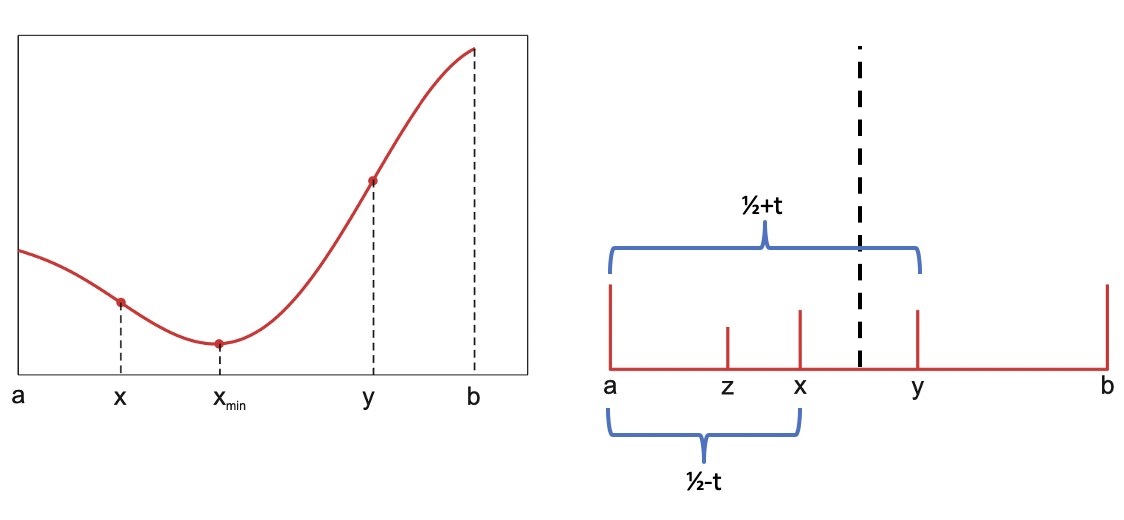
\includegraphics[width=16cm, height=6cm]{images/im221.png}
    \label{ris:im221}
    \caption{Слева: унимодальная функция, справа: точки, выбираемые по золотому сечению}
\end{figure}

\subsubsection{Метод золотого сечения}
В методе золотого сечения точки внутри интервалов поиска решения выбираются исходя из следующих предложений:
\begin{itemize}
    \item на текущей итерации оба потенциальных интервала сокращения равны между собой;
    \item на каждой итерации интервал сокращается на одну и ту же величину.
\end{itemize}
Эти два предложения позволяют однозначно определить процесс генерации новых точек. Предположим, что текущий интервал поиска [a, b] имеет единичную длину и в нём выбраны две точки x, y (см. рисунок \ref{ris:im221}, справа). Равенство потенциальных интервалов сокращения означает, что длина  $[a, x]$ равна $1/2 - t$, а длина $[a, y] - 1/2 + t$, где $t$ – некоторая неизвестная величина.
\newline \newline Пусть на текущей итерации выбирается интервал [a, y] и на следующей итерации к точке x добавляется точка z. Тогда предложение о сокращении интервалов на фиксированную величину означает, что:
$$\dfrac{l[a, y]}{l[a, b]}=\dfrac{l[a, x]}{l[a, y]}=K,$$
где через $l[a, y]$ обозначена длина интервала $[a, y]$. В результате получаем:
$$\dfrac{1/2+t}{1}=\dfrac{1/2-t}{1/2+t} \Rightarrow t = \dfrac{\sqrt{5}-2}{2} \Rightarrow K = \dfrac{\sqrt{5}-1}{2}$$
\newline
\begin{figure}[hbt!]
    \centering
    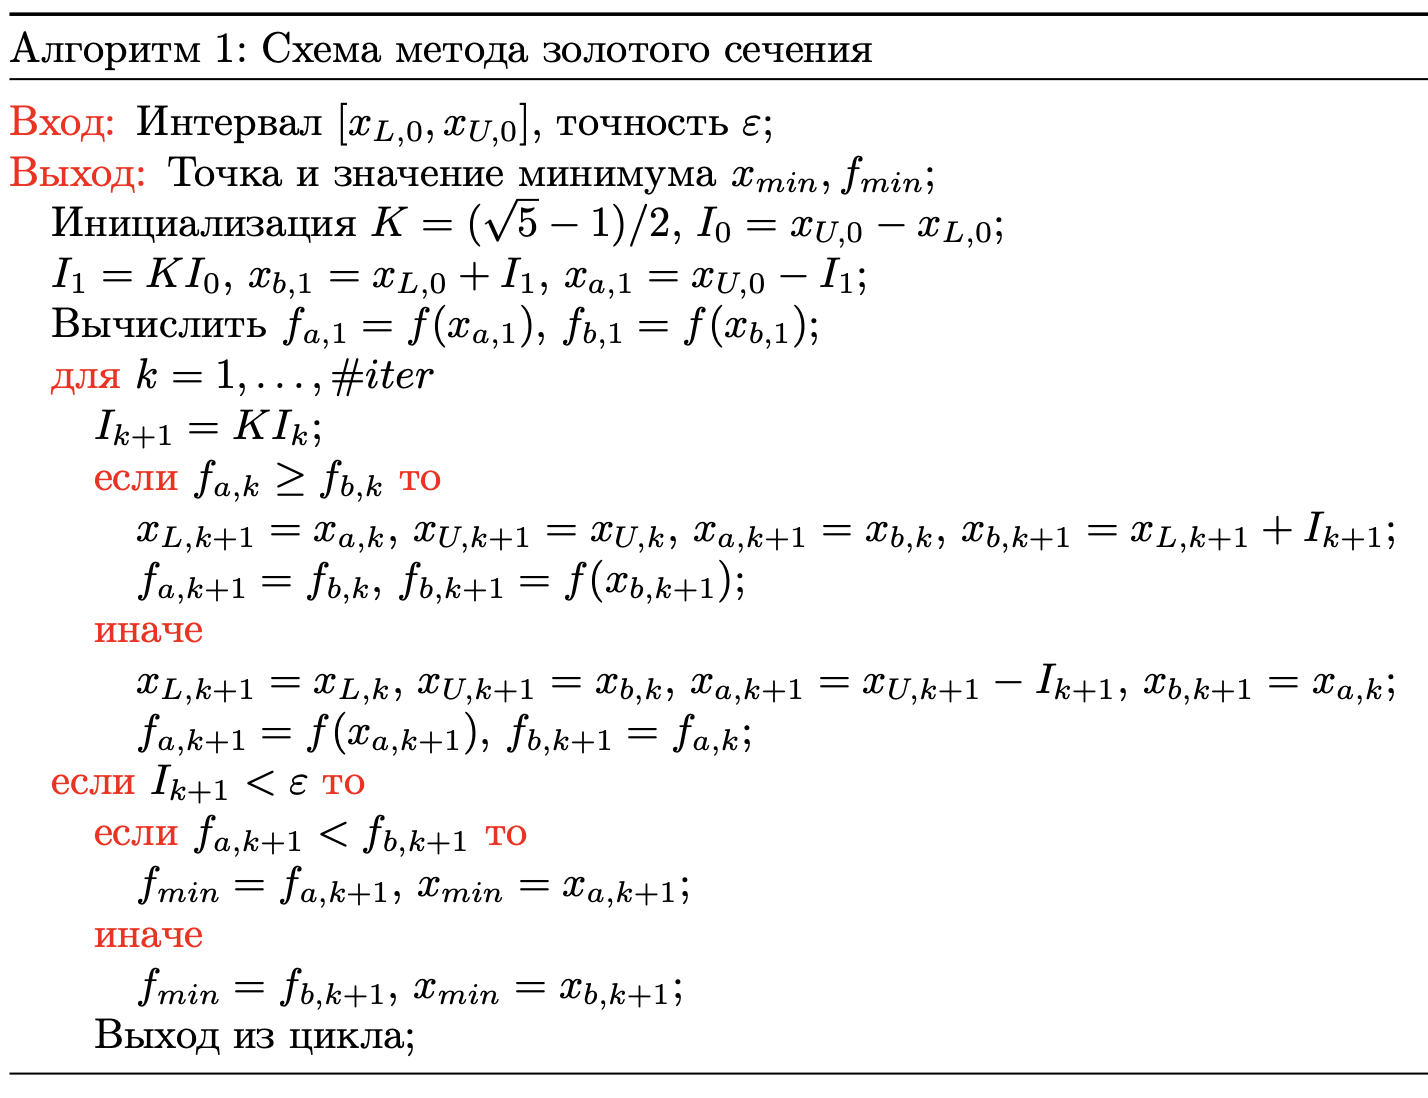
\includegraphics[width=14cm, height=10cm]{images/im222.png}
    \label{ris:im222}
    \caption{Алгоритм 1: Схема метода золотого сечения}
\end{figure}
Схема метода золотого сечения представлена в Алгоритме 1 (см. рисунок \ref{ris:im222}). В этой схеме границы интервала на итерации k обозначены как $x_{L,k}$ и $x_{U,k}$, длина интервала как $I_k$, а две внутренние точки интервала как $x_{a,k}$ и $x_{b,k}$.
Очевидно, что длина интервала $I_k = KI_{k-1} = K^2I_{k-2} = \dots = K^kI_0$, где $I_0$ – длина начального интервала, заданного пользователем. Поэтому \textbf{скорость сходимости} метода золотого сечения является \textbf{линейной} с константой $K$. Кроме того, из условия $ K^kI_0 \textless \varepsilon$  можно определить количество итераций, которые потребуются методу для достижения точности $\varepsilon$. Заметим также, что в методе золотого сечения оптимизируемая функция $f$ \textbf{не вычисляется в крайних точках} $x_{L,0}$ и $x_{U,0}$. Это удобно, например, для оптимизации функций с вертикальными асимптотами.

\subsubsection{Метод парабол}
\begin{figure}[hbt!]
    \centering
    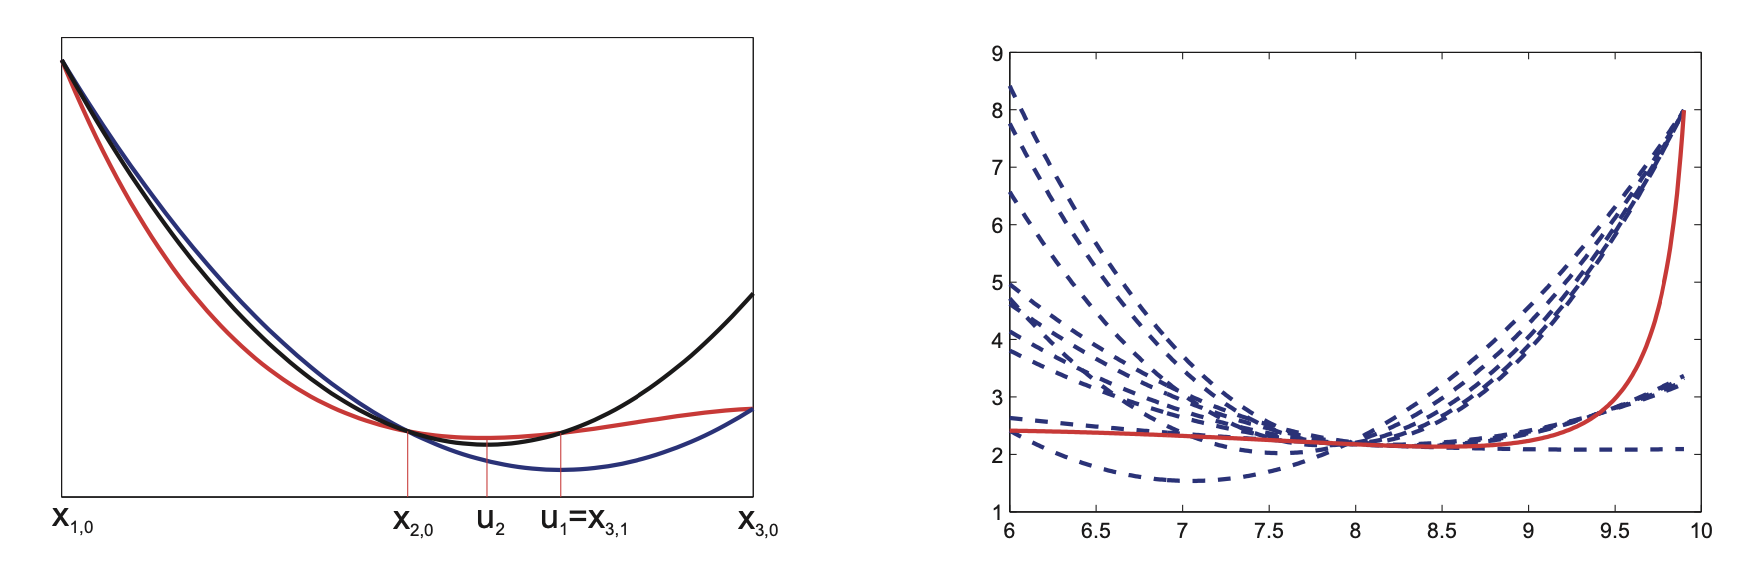
\includegraphics[width=16cm, height=6cm]{images/im223.png}
    \label{ris:im223}
    \caption{ Иллюстрация работы метода парабол. Слева: первые две итерации метода, красная кривая – оптимизируемая функция, синяя кривая – квадратичное приближение на первой итерации, чёрная кривая – квадратичное приближение на второй итерации. Справа: пример плохой сходимости метода парабол, красная кривая – оптимизируемая функция, синие кривые – итерационные квадратичные приближения.}
\end{figure}
В методе парабол предлагается аппроксимировать оптимизируемую функцию $f(x)$ с помощью квадратичной функции:
$$p(x)=ax^2 +bx+c.$$
Пусть имеются три точки $x_1 < x_2 < x_3$ такие, что интервал $[x_1,x_3]$ содержит точку минимума функции $f$. Тогда коэффициенты аппроксимирующей параболы $a, b, c$ могут быть найдены путем решения системы линейных уравнений:
$a x^2_i + bx_i + c = f_i = f ( x_i ) , \ i = 1 , 2 , 3 .$
Минимум такой параболы: $u = -\dfrac{b}{2a}$.
\newline \newline
Если $f(x_2) < f(x_1)$ и $f(x_2) < f(x_3)$, то точка $u$ гарантированно попадает в интервал $[x_1,x_3]$. (см. рисунок \ref{ris:im223}, слева).
\begin{center}
    Если $f(u)\leq f(x_2)$, то $[x_1, x_3] \to [x_1, x_2]$, иначе $[x_1, x_3] \to [u, x_3]$.
\end{center}
В отличие от метода золотого сечения, метод парабол обладает \textbf{суперлинейной скоростью сходимости}. Однако, такая высокая скорость сходимости гарантируется только \textbf{в малой окрестности точки минимума $x_{min}$}. На начальных стадиях процесса оптимизации метод парабол может делать очень маленькие шаги или, наоборот, слишком большие шаги, приводящие к неустойчивым биениям (см. рисунок \ref{ris:im223}, справа). Также следует отметить, что на первой итерации метод парабол \textbf{требует измерения значений функции f в крайних точках} интервала оптимизации.

\subsubsection{Комбинированный метод Брента}
Метод золотого сечения представляет собой надежный способ оптимизации, который сходится за гарантированное число итераций, но обладает лишь линейной скоростью сходимости. Метод парабол работает быстрее в малой окрестности оптимального решения, но может работать долго и неустойчиво на начальных стадиях итерационного процесса. Поэтому на практике для решения задачи одномерной оптимизации используется метод Брента, который эффективно комбинирует эти две стратегии.
\newline \newline В данном методе на каждой итерации отслеживаются значения в шести точках (не обязательно различных): $a, c, x, w, v, u$.
\newline \newline Точки $a, c$ задают текущий интервал поиска решения,
\newline $x$ – точка, соответствующая наименьшему значению функции,
\newline$ w $ – точка, соответствующая второму снизу значению функции,
\newline $v$ – предыдущее значение$ w$.
\newline \newline В отличие от метода парабол, в методе Брента аппроксимирующая парабола строится с помощью трех наилучших точек $x, w, v $(в случае, если эти три точки различны и значения в них также различны). При этом минимум аппроксимирующей параболы $u$ принимается в качестве следующей точки оптимизационного процесса, если:
\begin{itemize}
    \item $u$ попадает внутрь интервала $[a, c]$;
    \item $u$ отстоит от точки $x$ не более, чем на половину от длины предпредыдущего шага.
\end{itemize}
Если точка $u$ отвергается, то следующая точка находится с помощью золотого сечения большего из интервалов $[a, x] $и $[x, c]$. Итоговая схема Брента представлена в Алгоритме 2. (см. рисунок \ref{ris:im224})
\begin{figure}[hbt!]
    \centering
    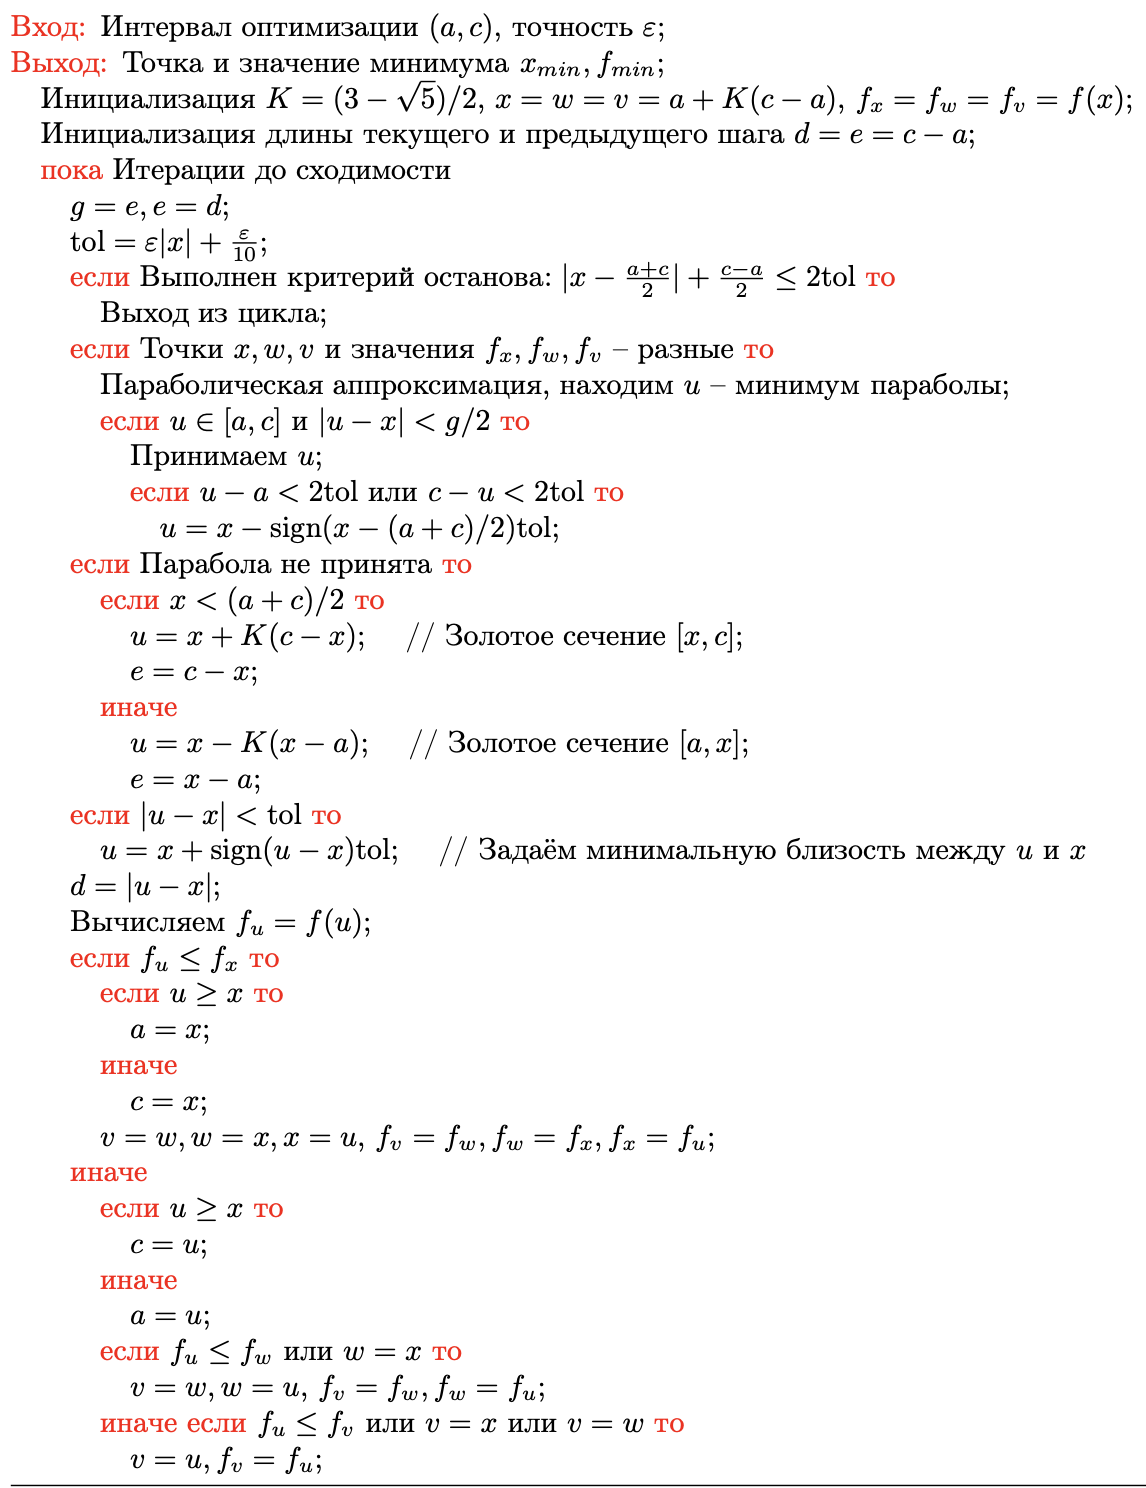
\includegraphics[width=14cm, height=19cm]{images/im224.png}
    \label{ris:im224}
    \caption{Алгоритм 2: Комбинированный метод Брента}
\end{figure}
\newline  \newline
Приведем некоторые аргументы в пользу обозначенных условий приема минимума параболы $u$. Так как парабола на текущей итерации проводится через точки $x,w,v$, для которых не гарантируются соотношения $v < x < w$ или $w < x < v$, то минимум параболы может оказаться вне интервала $[a,c]$. Ограничение на максимальную удалённость $u$ от $x$ позволяет избежать слишком больших шагов в оптимизации, которые могут соответствовать биениям в методе парабол. Использование в данном ограничении длины предпредыдущего шага, а не предыдущего, является эвристикой, эффективность которой подтверждается в экспериментах на больших базах задач оптимизации. Эта эвристика предлагает не штрафовать метод за текущий не слишком удачный маленький шаг в надежде на успешные шаги метода на следующих итерациях.

\subsubsection{Неточная одномерная оптимизация}
Во многих методах многомерной оптимизации на итерации k имеется текущая точка $x_k \in \mathbb{R}^n$ и некоторое направление минимизации $d_k \in \mathbb{R}^n$ . Тогда следующая точка итерационного процесса $x_{k+1}$ находится путем решения следующей задачи одномерной оптимизации:
\begin{equation}
    \label{formula222}
    \phi(\alpha) = f(x_k+\alpha d_k)\to \min_{\alpha \geq 0}.
\end{equation}
Эту задачу можно решать с помощью методов, описанных выше. Однако, для сходимости общего процесса многомерной оптимизации задачу \ref{formula222} зачастую не обязательно решать точно. На практике здесь оказывается достаточным лишь значимо уменьшить значение функции на текущей итерации. Отказ от точного решения  \ref{formula222}  позволяет во многих случаях сократить количество обращений к оракулу.
\newline
Итак, дано:
$$\phi(\alpha) = f(x_k+\alpha d_k)$$
$$\phi'(0) = \nabla f(x_k)^T d_k < 0$$
Условия неточной одномерной оптимизации:
\begin{itemize}
    \item[1.] \textbf{Условие Армихо.}
    Гарантирует уменьшение значения функции на текущей итерации (условие, значимого уменьшения). См. рисунок \ref{ris:im225} слева.
    $$\phi(\alpha_k) \leq \phi(0) + c_1 \alpha_k \phi'(0), c_1 \in (0,1) $$

    \item[2.] \textbf{Условие Вольфа.} Есть два условия - слабое и сильное, мы используем одно из двух. См. рисунок \ref{ris:im225} справа. \newline
    \begin{itemize}
        \item[a.] (слабое условие) $\phi'(\alpha_k)\geq c_2 \ \phi'(0), \ c_2 \in (0,1)$
        \item[b.] (сильное условие) $|\phi(\alpha_k)|\leq c_2 \ |\phi'(0)|, \ c_2 \in (0,1)$
    \end{itemize}
    Сильное условие Вольфа позволяет эффективно локализовывать минимум: если константу $c_2$ начинаем стремить к 0, мы все сильнее сжимаем интервал (на рис. между голубой и красной точками) и гарантируем то, что $\alpha_k$, удовлетворяющая сильному условию, будет приблеженным точным оптимумом при $c_2 \to 0$.
    \begin{figure}[hbt!]
        \centering
        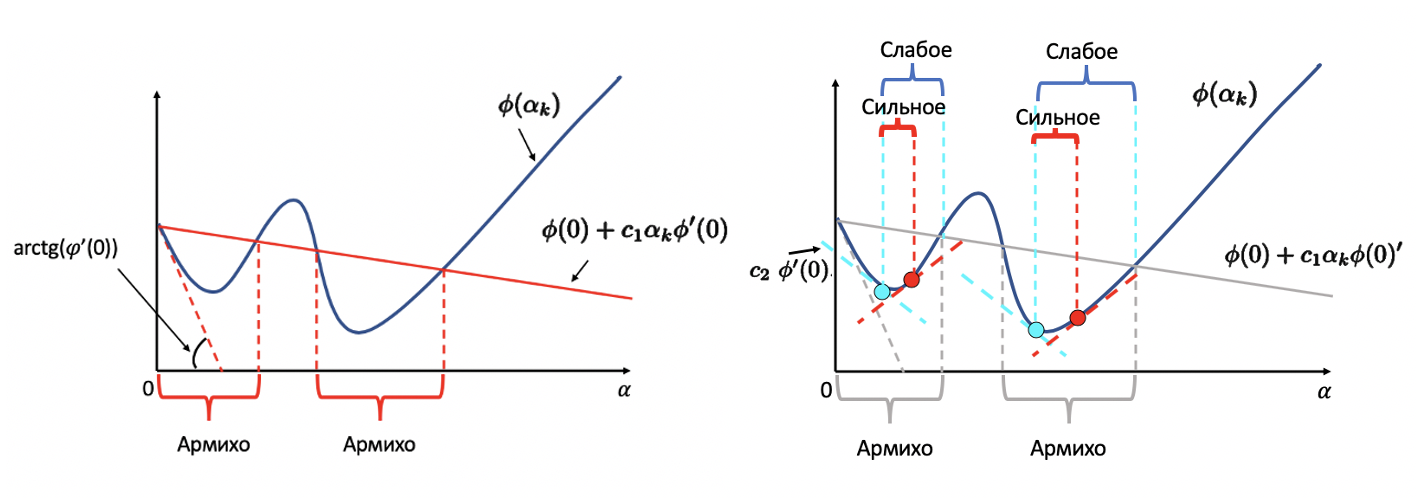
\includegraphics[width=16cm, height=6cm]{images/im225.png}
        \caption{Иллюстрация достаточных условий для неточной одномерной минимизации. Слева: условие Армихо, справа: слабое/сильное условие Вольфа.}
        \label{ris:im225}
    \end{figure}
    \newline
    На практике берут $c_1=10^{-4}, \ c_2 = 0.9$ (если интересует незначительное уменьшение функции) или $c_2=0.1$ (если важно посильнее минимизировать функцию)
\end{itemize}
\textbf{Теорема.}
Если $\phi(\alpha)\in C^1, \ \phi'(\alpha)<0, \phi(\alpha)>-\infty \ \forall \alpha$ и
$0<c_1\leq c_2<1 \Rightarrow$ \newline
$\exists \alpha_*,$ удовлетворяющая условию Армихо и слабому или сильному условию Вольфа.
\newline \textbf{Доказательство.}
$$\phi(\alpha)=\phi(0)+\phi'(0) \alpha + o(\alpha^2) \leq \phi(0)+c_1\alpha\phi'(0)$$
$$\phi'(0)+o(\alpha)\leq c_1 \phi'(0)$$
$$\underbrace{\underbrace{(1 -c_1)}_{\text{>0}}\underbrace{\phi'(0)}_{\text{<0}}}_{\text{<0}}+o(\alpha)\leq 0$$
\begin{center}
    $=> \exists \alpha_*: \forall \alpha \in (0, \alpha_*)$
    условие Армихо выполнено.
\end{center}
$$\exists \hat{\alpha} \ : \ \phi(\hat{\alpha})=\phi(0)+c_1 \hat{\alpha}  \phi'(0)$$
$$\psi(\alpha) := \phi(\alpha)-\phi(0)-c_1\alpha\phi'(0) $$
\begin{center}
    $\psi(0)=0; \ \psi(\hat{\alpha})=0$
    и т. к. $\alpha_*$ лежит между 0 и $\hat{\alpha} => \exists \alpha_* : \ \psi'(\alpha_*)=0$
\end{center}
$$\psi'(\alpha_*)=\phi'(\alpha_*)-c_1 \phi'(0)=0 $$
$$=> \ \phi'(\alpha_*)=c_1 \underbrace{\phi'(0)}_{<0} \geq c_2 \phi'(0)$$
\begin{center}
    $=> \ \alpha_*$ удовлетворяет слабому условию Вольфа.
\end{center}
$$|\phi'(\alpha_*)|=|c_1\phi'(0)|\leq c_2 |\phi'(0)|$$
\begin{center}
    $=> \ \alpha_*$ удовлетворяет сильному условию Вольфа.
\end{center}
\hfill$\scriptstyle\blacksquare$
\textbf{Алгоритм поиска $\alpha_*$.}
\begin{itemize}
    \item[1.] \textbf{Расширение (поиск правой границы)} \\
    Пользователь задает начальную точку $\alpha_0$. Сначала нужно найти интервал, в котором находится искомая точка, т.е. берется точка $\alpha_0$ и умножается на некоторую константу (сдвигается вправо) пока не будет выполнено одно из условий для правой границы.
    \item[2.] \textbf{Сужение} \\
    Теперь интервал нужно сужать:
    \begin{itemize}
        \item[i.] Внутри текущего интервала генерируем (через метод парабол или золотого сечения) какую-то точку
        \item[ii.] Проверяем для нее условия Армихо и Вольфа, если они не выполнены, то сдвигаем интервал налево или направо по условиям для правой и левой границ.
        \item[iii.] Сужаем интервал пока не найдем нужную точку.
    \end{itemize}
\end{itemize}
\textbf{ Условия для правой границы:}
\begin{itemize}
    \item[1.] Не выполнено условие Армихо
    \item[2.] $\phi'(\alpha)>0$ и не выполнено условие Вольфа
    \item[3.] $\phi(\alpha)>\phi(\alpha_{prev})$
\end{itemize}
\textbf{ Условие для левой границы:} в левой точке $\phi'(\alpha)<0$

    \subsection{Метод градиентного спуска. Стратегии выбора длины шага. Скорость сходимости метода для сильно выпуклых функций, примеры быстрой и медленной работы метода. @juliasemavina}

    Обозначения:
\begin{itemize}
    \item $C_L^{p,k} (Q)$ - класс функций со следующими свойствами:
    \begin{enumerate}
        \item $f(x)$ $k$ раз непрерывно дифференцируема на $Q$.
        \item  p-ая производная функции $f$ удовлетворяет условию Липшица на $Q$ с константой $L$:
        $$\forall x, y \in Q \text{ } ||f^{(p)}(x) - f^{(p)}(y)|| \leqslant L||x-y||$$
    \end{enumerate}
    \item $\mathscr{F}^1(Q)$ -
    класс функций, выпуклых на множестве $Q$.
    \item $\mathscr{F}_L^{p,k}(Q)$ -
    подкласс выпуклых на $Q$ функций
    класса
    $C_L^{p,k} (Q)$.
    \item $\mathscr{T}_{\mu}^{1} (Q)$ -
    класс функций, сильно выпуклых на множестве $Q$ с коэффициентом $\mu$.
    \item $\mathscr{T}_{\mu, L}^{p,k}(Q)$ -
    подкласс  сильно выпуклых  с коэффициентом $\mu$ на $Q$ функций
    класса
    $C_L^{p,k} (Q)$.

\end{itemize}

Будем решать задачу гладкой выпуклой безусловной минимизации:
\begin{equation*}
    \min\limits_{x \in \mathbb{R}^n} f(x)
\end{equation*}
где
$f \in C_L^{1,1}(\mathbb{R}^n)$,
то есть f - непрерывно дифференцируемая  с липшицевой первой производной.

\subsubsection{Метод градиентного спуска}

\begin{figure}[H]
            \centering
            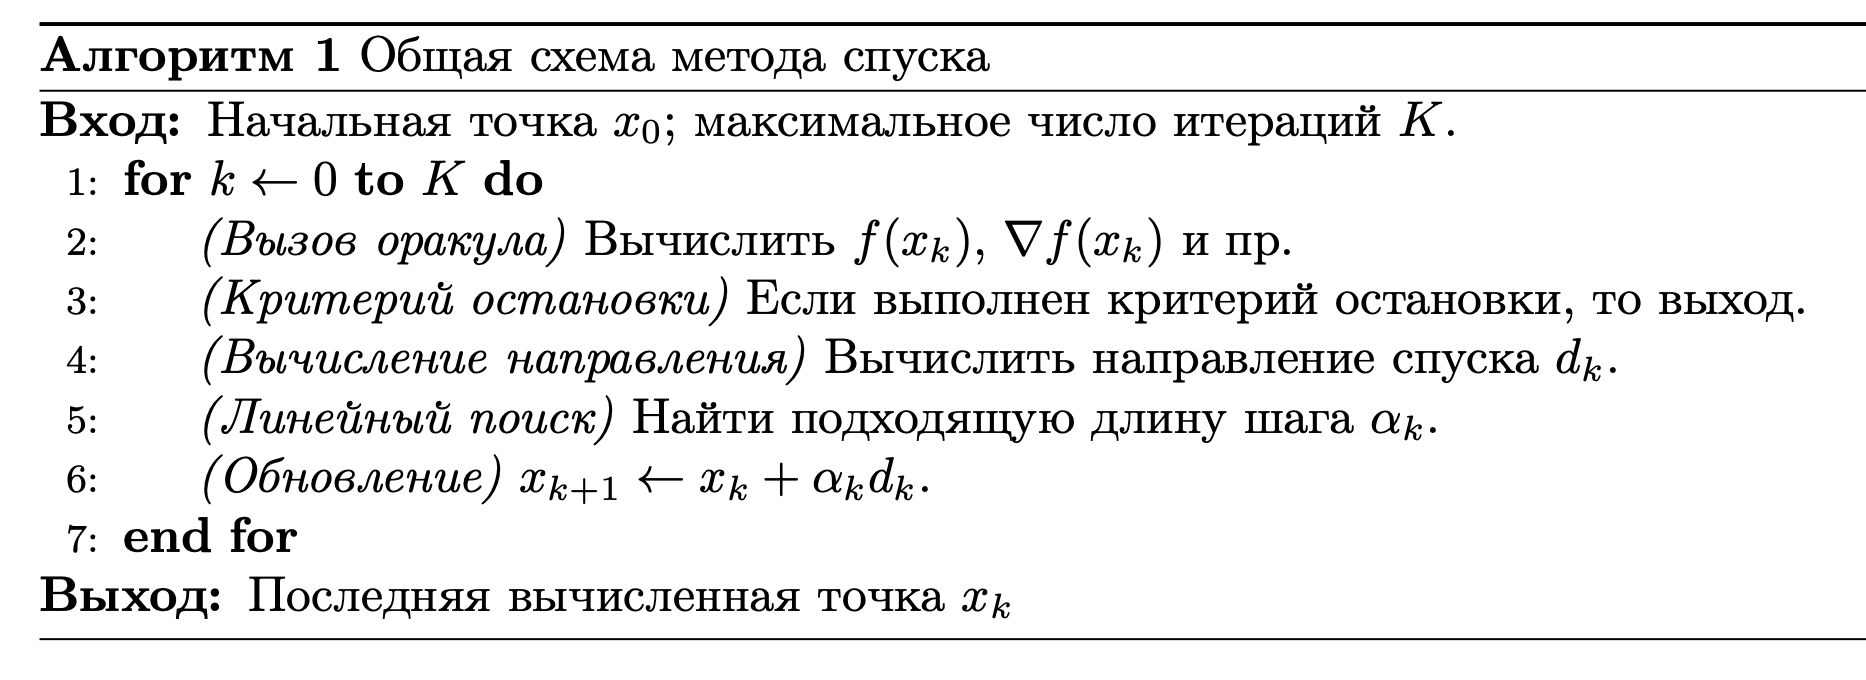
\includegraphics[width=16cm, height=6cm]{images/2-3-grad.png}
            \label{ris:im225}
            \caption{Метод спуска}
        \end{figure}

В случае градиентного спуска достаточно двух оракулов
$f(x_k)$ и
$\nabla f(x_k)$,
а в качестве направления  выбирается направление наискорейшего спуска:
$d_k = -\nabla f_k(x)$.

\subsubsection{Стратегии выбора длины шага
($\alpha_k$)}

Мы решаем подзадачу нахождения
$x_{k+1} = x_k - \alpha_k d_k$  в методе градиентного спуска. Нам бы хотелось найти такую точку $x_{k+1}$ которая бы давала значительное уменьшение целевой функции.
То есть наша задача состоит в минимизации функции
\begin{equation*}
    \phi_k(\alpha_k) = f(x_k + \alpha_k d_k)
\end{equation*}
Рассмотрим различные стратегии выбора длины шага:

\begin{enumerate}
    \item {\bf Последовательность
    $\{\alpha_k\}$ задана заранее.}

    Например:
    \begin{itemize}
        \item  $\alpha_k = \alpha > 0$ - константный шаг.
        Не гарантирует сходимость для всех гладких выпуклых функций. Сходимость гарантируется, если
        $\alpha \leqslant \frac{1}{L}$ и функция имеет липшицев градиент.
        \item  $\alpha_k = \frac{\alpha}{\sqrt{k+1}}$
        \item $\{\alpha_k\}$ такова,  что ряд
        $\sum \alpha_k$ расходится, а ряд $\sum \alpha_k^2$ сходится.         (ШАД 2019 Введение в методы оптимизации).
        Такие последовательности обеспечивают сходимость метода градиентного спуска для любых выпуклых гладких функций.
    \end{itemize}

    Применение:
    Очень простой метод, чаще всего применяется для задач выпуклой оптимизации.
    \item {\bf Полная релаксация} -
    $\alpha_k =  \argmin\limits_{\alpha > 0} f(x_k - \alpha \nabla f(x_k))$

    В этом случае можно использовать любые методы одномерной оптимизации, однако, точно эта задача обычно не решается.

    Применение:
    Имеет исключительно теоретический интерес, не применяется на практике.

    \item {\bf Бэктрекинг} - Метод дробления шага.
    Уменьшаем длину шага в фиксированное количество раз, пока не выполняется некоторое условие. В качестве условий часто применяются условия Армихо и Вульфа.

    Условие Армихо:
    $
        \phi_k (\alpha_k) \leqslant \phi_k(0) + c_1 \alpha \phi'_k(0), c_1 \in (0, 1)
    $

        Условия Вульфа:
    $
        \phi_k (\alpha_k) \leqslant \phi_k(0) + c_1 \alpha \phi'_k(0),
        \phi'_k (\alpha_k) \geqslant c_2 \alpha \phi'_k(0),
        0 < c_1 < c_2 < 1
    $

    Сильные условия Вульфа:

    \quad \quad $
        \phi_k (\alpha_k) \leqslant \phi_k(0) + c_1 \alpha \phi'_k(0),
        |\phi'_k (\alpha_k)| \leqslant c_2 \alpha |\phi'_k(0)|,
        0 < c_1 < c_2 < 1
    $


    \begin{figure}[H]
            \minipage{0.45\textwidth}
            \centering
            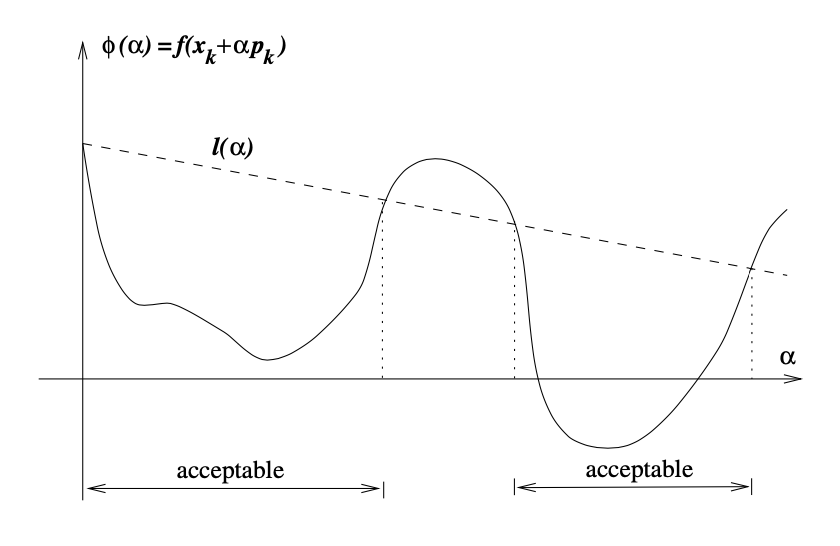
\includegraphics[scale=0.5]{images/2-3-armijo.png}
            \label{ris:im225}
            \caption{Иллюстрация к условию Армихо:
            Накладывает условие достаточного уменьшения функции.}
            \endminipage\hfill
            \minipage{0.45\textwidth}
            \centering
            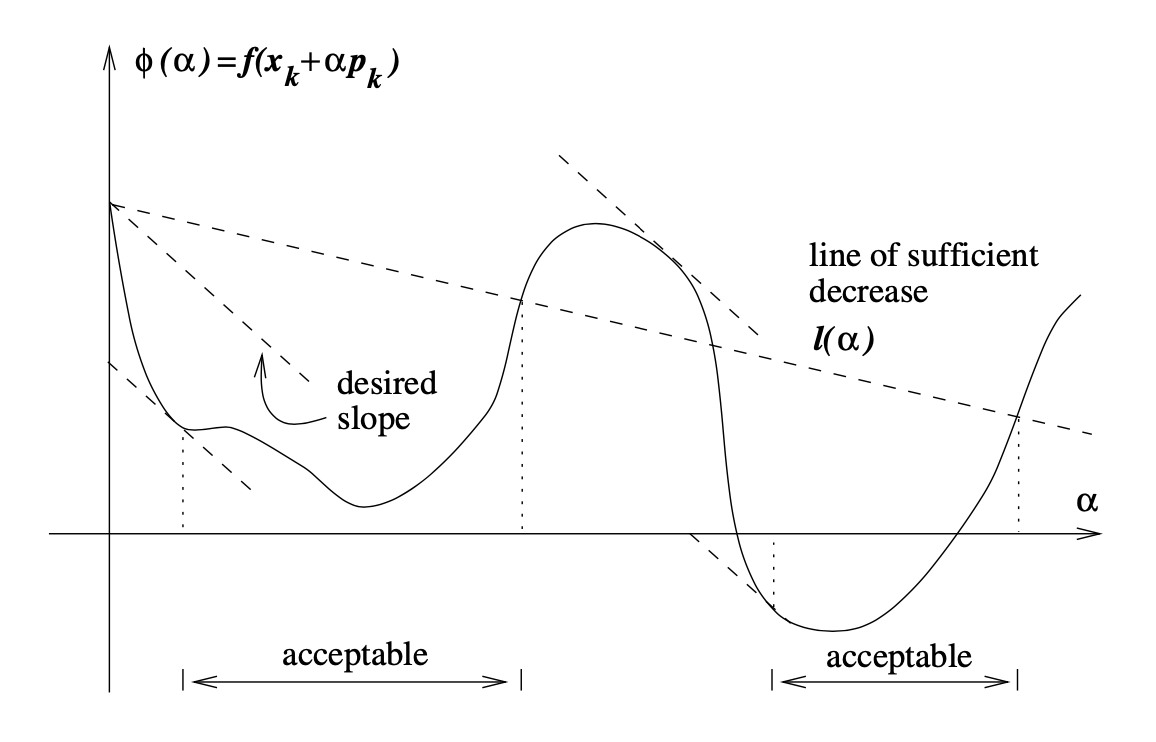
\includegraphics[scale=0.36]{images/2-3-wolfe.png}
            \label{ris:im225}
            \caption{Иллюстрация к условиям Вульфа: условие Армихо и
            условие кривизны функции: наклон не должен быть меньше начального, умноженного на константу.}
            \endminipage\hfill
    \end{figure}



    \begin{figure}[H]
            \centering
            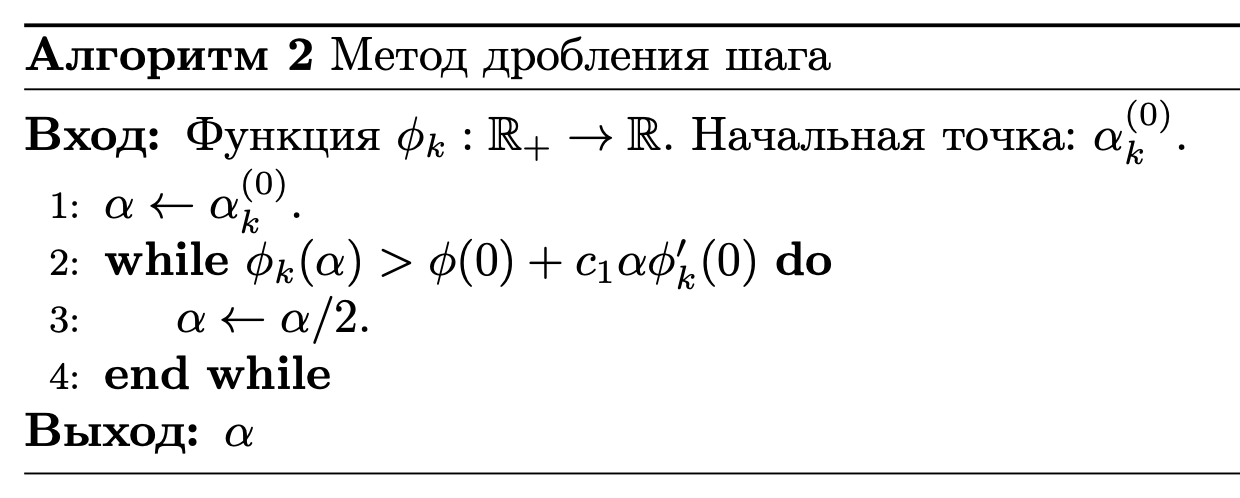
\includegraphics[width=16cm, height=6cm]{images/2-3-backtracking.png}
            \label{ris:im225}
            \caption{Процедура бэктрекинга с условием Армихо}
        \end{figure}


\end{enumerate}


\subsubsection{Скорость сходимости метода для сильно выпуклых функций }

{\bf Лемма 1}
Пусть
$f \in \mathscr{T}_{\mu, L}^{1,1}(\mathbb{R}^n)$.
Тогда
$\forall x, y \in \mathbb{R}^n$:

\begin{equation*}
    \langle
         \nabla f(x) - \nabla f(y), x-y
    \rangle
    \geqslant
    \frac{\mu L}{\mu + L} ||x-y||^2 +
    \frac{1}{\mu + L} ||\nabla f(x) - \nabla f(y)||^2
\end{equation*}

{\bf Лемма 2}
Пусть
$f \in \mathscr{F}_{L}^{1,1}(\mathbb{R}^n)$.
Тогда
$\forall x, y \in \mathbb{R}^n$:
\begin{equation*}
    0 \leqslant f(y) - f(x) -
    \langle
         \nabla f(x), y-x
    \rangle
    \leqslant \frac{L}{2} ||x-y||^2
\end{equation*}

{\bf Теорема (Скорость сходимости градиентного метода):}
Пусть
$f \in \mathscr{T}_{\mu, L}^{1,1}(\mathbb{R}^n)$,
$0 < h \leqslant \frac{2}{\mu + L}$.
Тогда градиентный метод с константным шагом $h$ образует такую последовательность
$\{x_k\}$, что
\begin{equation*}
    ||x_k - x^*||^2 \leqslant
    \left(
        1 - \frac{2h\mu L}{\mu + L}
    \right)^k
    ||x_0 - x^*||^2
\end{equation*}
При этом, если $h=\frac{2}{\mu + L}$,
обозначив
$Q_f = \frac{L}{\mu}$:
\begin{equation*}
    ||x_k - x^*|| \leqslant
    \left(
        \frac{Q_f - 1}{Q_f + 1}
    \right)^k
    ||x_0 - x^*||
\end{equation*}
\begin{equation*}
    f(x_k) - f^* \leqslant
    \frac{L}{2}
    \left(
        \frac{Q_f - 1}{Q_f + 1}
    \right)^{2k}
    ||x_0 - x^*||^2
\end{equation*}

{\bf Доказательство:}

Обозначим: $r_k = ||x_k - x^*||$.

\begin{align*}
r_{k+1}^2 = ||x_{k+1} - x^*||^2 = &
\Bigg [
    x_{k+1} = x_k - h \nabla f(x_k)
\Bigg]\\
= & ||x_k - x^* -  h \nabla f(x_k)||^2 =
\langle
    x_k - x^* -  h \nabla f(x_k), x_k - x^* -  h \nabla f(x_k)
\rangle = \\
=& r_k^2
- 2h \langle
    x_k - x^*, \nabla f(x_k)
\rangle
+ h^2 ||\nabla f(x_k)||^2 \leqslant
\Bigg [
    \text{Лемма 1}, \nabla f(x^*)=0
\Bigg]\\
\leqslant &
\left(
    1 - \frac{2h\mu L}{\mu + L}
\right)
r_k^2 +
h
\left(
    h - \frac{2}{\mu + L}
\right)
||\nabla f(x_k)||^2 \leqslant
\Bigg [
    h \leqslant \frac{2}{\mu + L}
\Bigg]\\
\leqslant &
\left(
    1 - \frac{2h\mu L}{\mu + L}
\right)
r_k^2  \leqslant
\Bigg [
   \text{индукция}
\Bigg]\\
\leqslant &
\left(
    1 - \frac{2h\mu L}{\mu + L}
\right)^{k+1}
||x_0 - x^*||^2
\end{align*}


Чтобы получить результаты при $h=\frac{2}{\mu + L}$,
необходимо подставить значение $h$ в формулу, получить первое неравенство и из него при помощи леммы 2 получить второе.


\begin{itemize}
    \item Отдельно отметим, что для класса
$\mathscr{F}_L^{p,k}(Q)$ у градиентного метода с константным шагом $\alpha = \frac{1}{L}$ сходимость  градиентного метода сублинейная.
\end{itemize}


\subsubsection{Примеры быстрой и медленной работы метода.}


Вспомним полученную нами скорость сходимости:

$Q_f = \frac{L}{\mu}$:
\begin{equation*}
    ||x_k - x^*|| \leqslant
    \left(
        \frac{Q_f - 1}{Q_f + 1}
    \right)^k
    ||x_0 - x^*||
\end{equation*}

Это означает, что скорость сходимости линейна, но зависит от $Q_f$, а именно, при $Q_f >> 1$ ($Q_f$ сильно больше 1) сходимость метода очень медленная: при $Q_f = 100 $:
$\frac{Q_f - 1}{Q_f + 1} \approx 0.98$,
$\left(
    \frac{Q_f - 1}{Q_f + 1}
\right)^{30} \approx 0.55$.


При $Q_f \approx 1$ сходимость метода быстрая: при $Q_f = 2 $:
$\frac{Q_f - 1}{Q_f + 1} = 0.33$,
$\left(
    \frac{Q_f - 1}{Q_f + 1}
\right)^{10} \approx 0.000015$.

Кроме того,
$Q_f$ - оценка числа обусловленности гессиана $f$.

\begin{itemize}
    \item  Число обучсловленности матрицы
$\mu(A) = ||A|| \times ||A^{-1}||$,     $||\cdot||$ - любая операторная форма - то есть число обусловленности зависит от выбора нормы.

Пример операторной нормы:
$||A|| = \max \{ ||Ax|| \text{ : } ||x|| = 1 \}$.
\end{itemize}


Получается, что чем ближе число обусловленности к 1, тем лучше работает метод.
В геометрическом смысле: при числе обусловленности, близком к 1, метод работает хорошо, а при больших числах обусловленности требуется сильно больше итераций:

В примерах $f(x) = \frac{1}{2} \langle Ax,x \rangle - \langle b,x \rangle$

\begin{figure}[H]
            \minipage{0.3\textwidth}
            \centering
            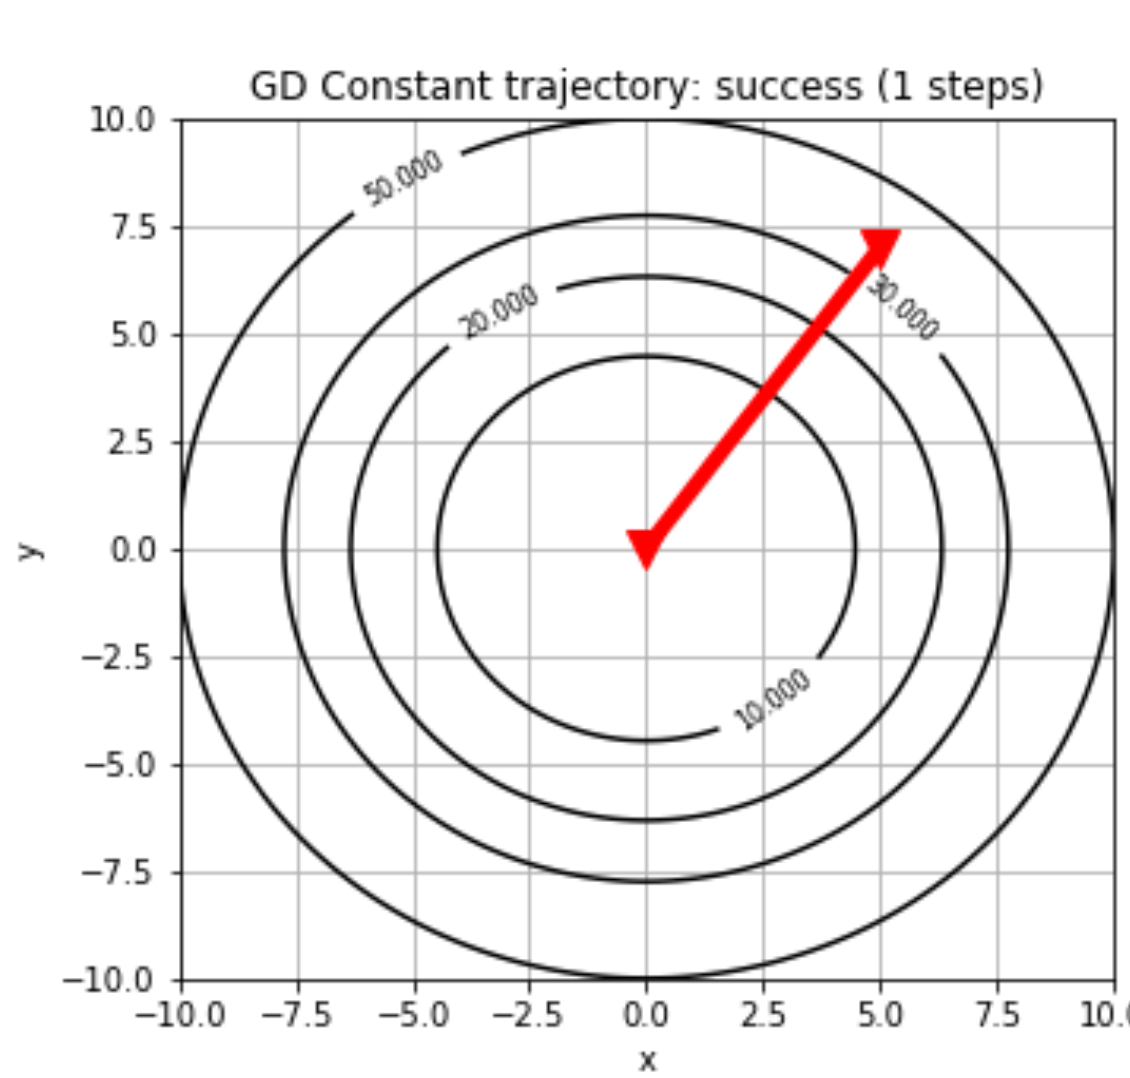
\includegraphics[scale=0.25]{images/2-3-traj1.png}
            \label{ris:im225}
            \caption{Число обусловленности $A$: 1}
            \endminipage\hfill
            \minipage{0.3\textwidth}
            \centering
            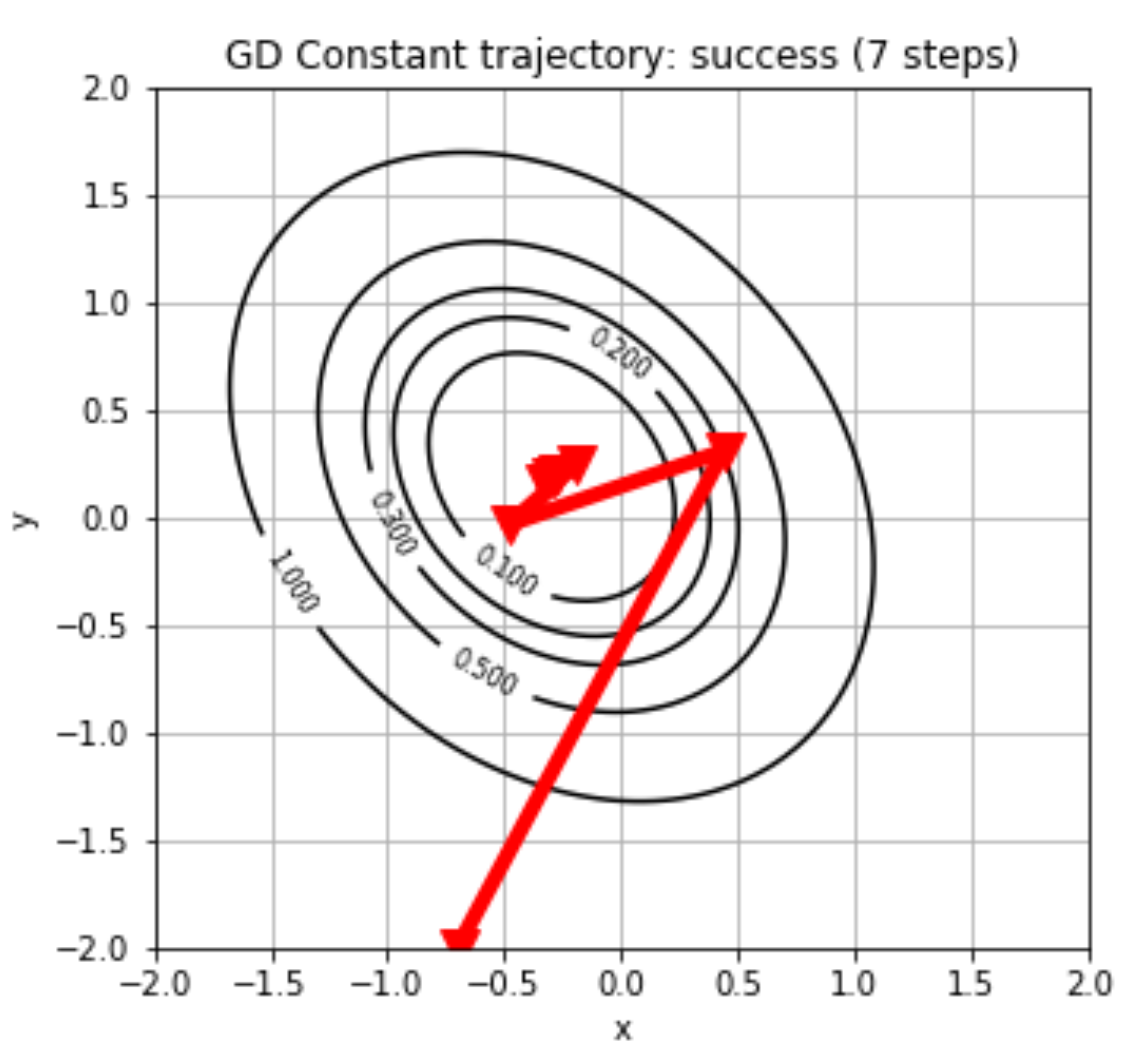
\includegraphics[scale=0.25]{images/2-3-traj2.png}
            \label{ris:im225}
            \caption{Число обусловленности $A$: 2}
            \endminipage\hfill
            \minipage{0.3\textwidth}
            \centering
            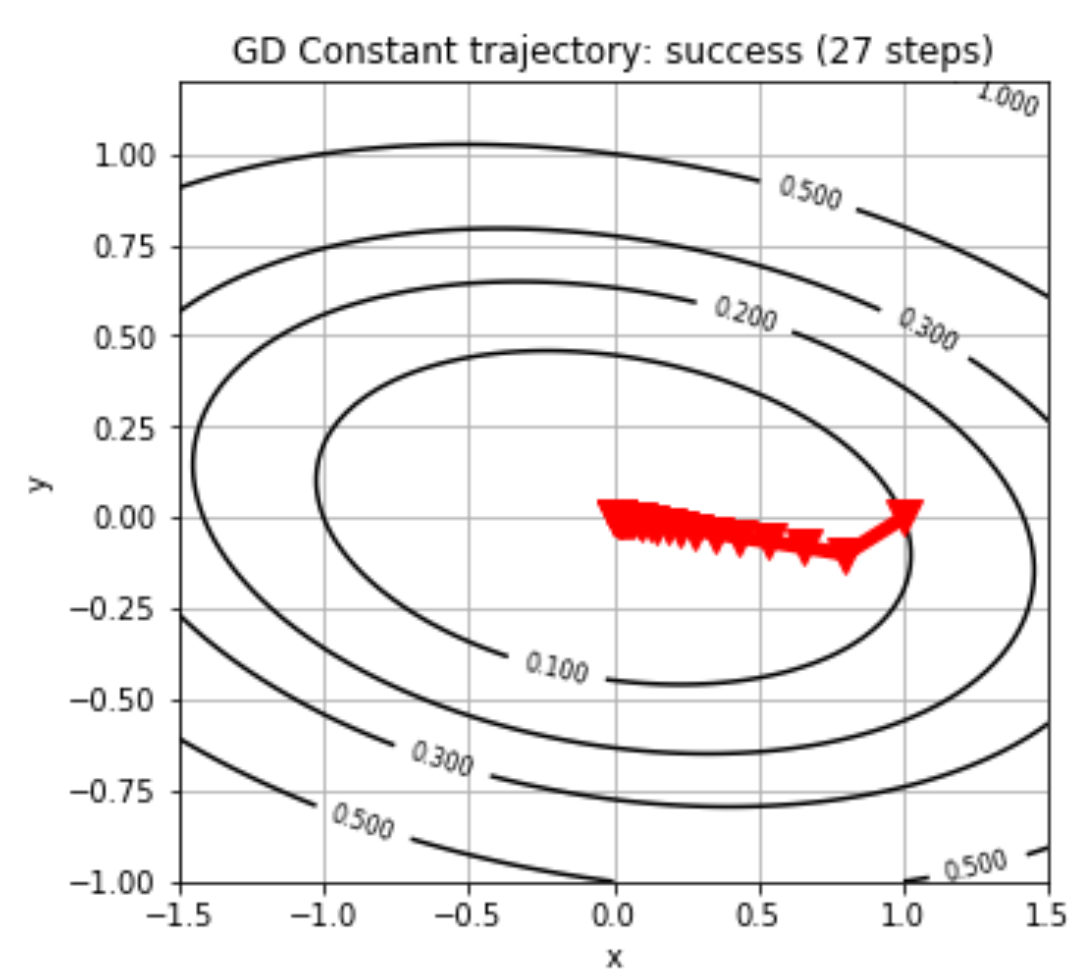
\includegraphics[scale=0.25]{images/2-3-traj6.png}
            \label{ris:im225}
            \caption{Число обусловленности $A$: 6.4}
            \endminipage\hfill
\end{figure}

    \subsection{Метод Ньютона, его локальная и глобальная скорость сходимости. Модификации метода Ньютона для невыпуклых задач оптимизации. Примеры быстрой и медленной работы метода. @Bitchert}

    \subsubsection{Метод Ньютона}
Рассмотрим нашу функцию в окрестности точки $x_k$, приблизим её некоторой квадратичной моделью $m_k(d_k)$:
\[
		f(x_k + d_k) \approx m_k(d_k) = f(x_k) + g_k^{T} d_k + \dfrac{1}{2} d_k^{T} B_k d_k \to \min\limits_{d_k}
\]
Для минимизации находим градиент модели и приравниваем к нулю:
\[
		\nabla_{d_k} m_k(d_k) = g_k + B_k d_k = 0 \Rightarrow d_k = - B_k^{-1} g_k
\]
Соответсвенно, если:
\begin{itemize}
		\item $g_k = \nabla f(x_k), \, B_k = \gamma_k I$ - получаем градиентный спуск
		\item $g_k = \nabla f(x_k), \, B_k = \nabla^2 f(x_k)$ - получаем метод Ньютона
\end{itemize}
Для метода Ньютона соответственно $f \in C^{2}$, и было бы неплохо, если $\nabla^2 f(x) \succ 0$, чтобы мы вообще куда-то оптимизировали:
\[
		d_k = - \left[ \nabla^2 f(x_k) \right]^{-1} \nabla f(x_k) \Rightarrow \dfrac{\partial}{\partial \alpha} f(x_k + \alpha d_k) \Big|_{\alpha = 0} = \nabla f(x_k)^{T} d_k = - \nabla f(x_k)^{T} \left[ \nabla^2 f(x_k) \right]^{-1} \nabla f(x_k)
\]
Последнее выражение, очевидно, меньше нуля для любых точек если $\nabla^2 f(x) \succ 0$. \\
Далее мы покажем глобальную сходимость метода Ньютона, его локальную сходимость и локальную скорость сходимости. \\
\subsubsection{Глобальная сходимость метода Ньютона}
Запишем условия Вульфа:
\[
		\begin{cases}
			f(x_k + \alpha_k d_k) \leq f(x_k) + c_1 \alpha_k \nabla f_k^{T} d_k \\
			\nabla f(x_k + \alpha_k d_k)^{T} d_k \geq c_2 \nabla f_{k}^{T} d_k
		\end{cases}
		\quad \text{где } 0 < c_1 < c2 < 1
\]
Косинус:
\[
		\cos \Theta_k = \dfrac{-\nabla f_k^{T} d_k}{\| \nabla f_k \|  \| d_k \|}
\]
\theorem{
Положим, что мы совершаем на каждом шагу итерации вида $x_{k + 1} := x_k + \alpha_k d_k$. Положим также, что $f$ ограничена снизу на $\mathbb{R}^{n}$ и $f \in C^{1, 1}_{L}$. Тогда:
\[
		\sum\limits_{k \geq 0} \cos^{2} \Theta_k \| \nabla f_k \|^2 < \infty
\]
}
\textbf{Доказательство:} \\
\[
		\nabla f(x_k + \alpha_k d_k)^T d_k - \nabla f_k^{T} d_k \geq (c_2 - 1) \nabla f_k^{T} d_k
\]
\[
		\left( \nabla f_{k + 1} - \nabla f_{k} \right)^{T} d_k \geq (c_2 - 1) \nabla f_k^{T} d_k
\]
Так как у $f$ липшицевый градиент:
\[
		\left( \nabla f_{k + 1} - \nabla f_{k} \right)^{T} d_k \leq \alpha_k L \| d_k \|^2
\]
Тогда, совмещая два предыдущих неравенства:
\[
		\alpha_k \geq \dfrac{c_2 - 1}{L} \dfrac{\nabla f_{k}^{T} d_k}{\| d_k \|^2}
\]
Подставляем в условие Вульфа (первое) и получаем:
\[
		f_{k + 1} \leq f_{k} - c_1 \dfrac{1 - c_2}{L} \dfrac{\left[\nabla f_{k}^{T} d_k\right]^2}{\| d_k \|^2} = f_k - c_1 \dfrac{1 - c_2}{L} \cos^2 \Theta_k \| \nabla f_k \|^2
\]
Теперь просуммируем по всем индексам до $k$:
\[
		f_{k + 1} \leq f_{0} - c_1 \dfrac{1 - c_2}{L} \sum\limits_{j=0}^{k} \cos^2 \Theta_k \| \nabla f_j \|^2
\]
Ну и так как функция ограничена снизу, то сумма ограничена сверху некой положительной константой.
\hfill$\scriptstyle\blacksquare$
\vspace{0.5cm}
\\
Из предыдущей теоремы вытекает, что
\[
		\cos^2 \Theta_k \| \nabla f_k \|^2 \to 0.
\]
Чтож, теперь остался маленький (!) трюк (!), который позволит доказать нам глобальную сходимость метода Ньютона. Для этого потребуем чтобы для матриц $B_k = \left[ \nabla^2 f_k \right]^{-1}$ числа обусловленности были ограничены: $\mu(B_k) \leq M \, \forall k, M > 0$ и все матрицы $B_k$ положительно определены. Теперь запишем косинус и попробуем его отделить от нуля: \\
\[
		\cos \Theta_k = \dfrac{\nabla f_k^{T} \left[ \nabla^2 f_k \right]^{-1} \nabla f_k}{\| \nabla f_k \| \| \left[ \nabla^2 f_k \right]^{-1} \nabla f_k \|}
\]
Рассмотрим отдельно норму произведения обратной матрицы гессиана на градиент:
\[
		\| \left[ \nabla^2 f_k \right]^{-1} \nabla f_k \| = \sqrt{ \nabla f_{k}^{T} \left[ \nabla^2 f_k \right]^{-2} \nabla f_{k} }  \leq \sqrt{\lambda_{max}\left(\left[ \nabla^2 f_k \right]^{-2}\right) \| \nabla f_k \|^2 } = \lambda_{max}\left(\left[ \nabla^2 f_k \right]^{-1}\right) \| \nabla f_k \|
\]
Тут мы используем микроскопический хитрый трюк: $\lambda_{min}(A) \leq x^T A x \leq \lambda_{max}(A)$ для $x^Tx = 1$. Тогда:
\[
	\cos \Theta_k \geq \dfrac{\lambda_{min}(\left[ \nabla^2 f_k \right]^{-1})}{\lambda_{max}(\left[ \nabla^2 f_k \right]^{-1})} \geq \dfrac{1}{M} > 0
\]
Таким образом, мы отделили косинус от нуля, значит последовательность норм градиентов стремится к нулю, что означает глобальную сходимость метода Ньютона для функций, у которых гессиан положительно определен во всех точках и имеет ограниченное сверху число обусловленности.
\subsubsection{Локальная сходимость метода Ньютона}
\theorem{
	Пусть $f \in C^{2, 2}_{M}$, $x_{*} - $ точка локального минимума с $\nabla^2 f(x_{*}) \succeq \mu I, \mu > 0$. Мы стартуем из некоторой окрестности точки $x_{*}$:
	\[
		x_0: \quad \| x_{*} - x_0 \| < \overline{r} = \dfrac{2\mu}{3M}
	\]
	Тогда метод Ньютона с $\alpha_k \equiv 1$ сходится $\| x_k - x_{*} \| < \overline{r} \, \forall k$ и имеет скорость сходимости квадратичную (суперлинейную):
	\[
		\| x_{k+1} - x_{*} \| \leq \dfrac{M \| x_{k} - x_{*} \|^2}{2 \left( \mu - M \| x_{k} - x_{*} \| \right)}
	\]
	}
\textbf{Доказательство:} \\
Мы делаем итерации вида $x_{k+1} = x_k - \left[ \nabla^2 f(x_k) \right]^{-1} \nabla f(x_k)$. Рассмотрим разность между $x_{k+1}$ и $x_{*}$:
\[
	x_{k+1} - x_{*} = x_{k} - x_{*} - \left[ \nabla^2 f(x_k) \right]^{-1} \nabla f(x_k) = x_k - x_{*} - \left[ \nabla^2 f(x_k) \right]^{-1} \int\limits_{0}^{1}\, \nabla^2 f(x_* + t(x_k - x_*))(x_k - x_*)  \, dt =
\]
\[
	= (x_k - x_*) \left[ \nabla^2 f(x_k) \right]^{-1} \int\limits_{0}^{1}\, \left( \nabla^2 f(x_k) - \nabla^2 f(x_* + t(x_k - x_*))\right) \, dt
\]
Положим $r_k := \| x_k - x_* \|$. Тогда:
\[
	\left\| \int\limits_{0}^{1}\, \left( \nabla^2 f(x_k) - \nabla^2 f(x_* + t(x_k - x_*))\right) \, dt \right\| \leq \int\limits_{0}^{1} \, \left\| \nabla^2 f(x_k) - \nabla^2 f(x_* + t(x_k - x_*)) \right\| \, dt \leq M \dfrac{r_k}{2}
\]
Так как для $f \in C^{2, 2}_{M}$ выполнено для $\| y - x \| = r$:
\[
	\nabla^2 f(x) - MrI_n \preceq \nabla^2 f(y) \preceq \nabla^2 f(x) + MrI_n,
\]
то:
\[
	\nabla^2 f(x_k) \succeq \nabla^2 f(x_*) - Mr_k I_n \succeq (\mu - Mr_k)I_n
\]
Тогда если $r_k < \dfrac{\mu}{M}$, то гессиан в точке $x_k$ положительно определен и $\left\| \left[\nabla^2 f(x_k)\right]^{-1} \right\| \leq (\mu - Mr_k)^{-1}$. Значит имеем:
\[
	r_{k + 1} \leq \dfrac{M r_{k}^2}{2(\mu - Mr_k)}
\]
Из этого следует, что для $x_0: \quad \| x_{*} - x_0 \| < \overline{r} = \dfrac{2\mu}{3M}$ метод Ньютона сходится и сходится квадратично (суперлинейно).
\hfill$\scriptstyle\blacksquare$
\subsubsection{Модификации метода Ньютона для невыпуклых задач оптимизации}
Для невыпуклых задач не выполняется $\nabla^2 f \succ 0$. Хотим теперь использовать в качестве $B_k$ какую-то матрицу, которую будем строить на основе гессиана, но чтобы она имела положительную определенность. Итерации нашего метода выглядят по-прежнему: $x_{k+1} = x_k - \alpha_k B_k^{-1}\nabla f(x_k)$. \\
Рассмотрим несколько методов коррекции гессиана для достижения положительной определенности:
\begin{itemize}
	\item \textbf{Модификация собственных значений} Так как гессиан симметричная матрица, то можем представить его в виде:
	\[
		\nabla^2 f(x_k) = Q \Lambda Q^T, \quad \Lambda = \Diag(\lambda_1, \dots, \lambda_n), \quad Q^{-1} = Q^{T}
	\]
	Тогда в качестве матрицы $B_k$ можно взять
	\[
		B_k = Q \overline{\Lambda} Q^{T}, \text{ где } \overline{\lambda_i} = \begin{cases}
		\lambda_i, \, \lambda_i \geq \delta > 0, \\
		\delta, \text{ иначе.}
		\end{cases}
	\]
	После того, как мы нашли собственное разложение, уже можно не решать заново СЛАУ $B_k d_k = -\nabla f(x_k)$, а в явном виде вычислить $d_k$:
	\[
		d_k = - Q \overline{\Lambda}^{-1} Q^{T} \nabla f(x_k)
	\]
	\item \textbf{Модификация диагонали} В качестве $B_k$ берём следующую матрицу:
	\[
		B_k = \nabla^2 f(x_k) + \tau_k I_n
	\]
	\begin{algorithmic}[1]
		\Procedure{\textsc{BkSearch}}{$f, x_k, \tau$}
		\State get $\nabla^2 f(x_k)$
		\While{$\tau < \tau_{max}$}
		\State $B_k \gets \nabla^2 f(x_k) + \tau I_n$
		\If{\textsc{CholeskyDecomposition($B_k$)}}
			\textbf{break}
		\EndIf
		\State $\tau \gets \min(\tau_{max}, \tau \nu), \, \nu > 1$
		\EndWhile
		\State $\tau \gets \tau / \beta, \, \beta > 1$
		\State \Return $B_k, \tau$
		\EndProcedure
	\end{algorithmic}
	Соответственно, если всё удачно, то мы знаем разложение Холецкого для нашей матрицы $B_k$ и для вычисления $d_k$ нужно дважды решить СЛАУ с треугольной матрицей:
	\[
		B_k = LL^{T} \Rightarrow d_k = - L^{-T} L^{-1} \nabla f(x_k)
	\]
	Это дешевле чем первый способ, потому что разложение Холецкого на порядок дешевле чем собственное разложение и даже несколько раз его выполнить будет дешевле одного собственного разложения.
	\item \textbf{Модификация симметричной факторизацией}
	Делаем разложение вида:
	\[
		P^{T} \nabla^2 f(x_k) P = LDL^{T}, \text{ где } L - \text{нижнетреугольная},\, D - \text{блочно-диагональная с блоками } 1\times1 \text{ и } 2\times2
	\]
	Тогда затем сделаем собственное разложение для $D$, это очень просто (блочно-диагональная матрица), потом сделаем модификацию для $\Lambda$ как мы делали в модификации собственных значений:
	\[
		B_k = PL\overline{D}L^{T}P^{T} \Rightarrow d_k = -PL^{-T}\overline{D}^{-1} L^{-1} P^{T} \nabla f(x_k)
	\]
\end{itemize}
\subsubsection{Примеры медленной и быстрой работы метода}
Идеальный вариант для работы метода Ньютона - квадратичная функция: $f(x) = \dfrac{1}{2} x^T A x + b^T x$, где $A \in \mathbb{S}^{n}_{++}, b \in \mathbb{R}^{n}$. Метод Ньютона сходится за одну итерацию из любой начальной точки. \\
В качестве функции, на который метод сходится линейно, можно назвать функцию $x^4$. \\
Плохой функцией можно назвать функцию Розенброка, на ней метод Ньютона вообще не сходится. \\
Еще можно упомянуть про большую размерность, что гессиан не будет влезать в память.

    \subsection{Метод сопряженных градиентов для решения системы линейных уравнений. Доказательство сходимости метода за конечное число итераций (в предположении, что сопряженные направления известны). Модификации метода для минимизации произвольных функций. @bigbluebutterfly}

    Преамбула: здесь мы построим итеративный, относительно легковесный и при этом точный метод решения СЛАУ с хорошими свойствами сходимости, а потом модифицируем его для оптимизации произвольных функций.

    Начнем с рассмотрения линейного метода сопряженных градиентов (далее CG). В сущности, это метод для решения СЛАУ вида $$Ax = b$$ где $A$ - симметричная положительно определенная матрица размера $n \times n$. Данную проблему, как известно, можно эквивалентно переформулировать в виде задачи оптимизации следующим образом: $$ \phi(x) = \frac{1}{2}\langle Ax, x\rangle - \langle b, x \rangle \to \min\limits_x$$
    Поскольку в обоих формулировках задача имеет одно и то же (притом единственное) решение, мы можем интерпретировать CG как метод решения СЛАУ или же как метод оптимизации выпуклых квадратичных функций. Отметим, что невязка СЛАУ $$r(x) = Ax-b$$ эквивалентна градиенту оптимизируемой функции: $$\nabla_x \phi(x) = Ax - b$$ В частности, на $k$-ом шаге: $$r_k = Ax_k - b$$Начнем немного издалека.

   \textbf{Определение.} Будем называть набор ненулевых векторов $\{ p_0, p_1,..., p_m\}$  \textbf{сопряженным} по отношению к симметричной положительно определенной матрице $A$, если
    \begin{align}
    p_i^T A p_j = 0, \ \ \ \  \forall i \neq j
    \end{align}
    Отметим, что такой набор векторов является линейно независимым. В самом деле, пусть $$\exists \alpha: \ \ \ \sum\limits_{i=0}^{n-1} \alpha_i p_i = 0$$
    Домножим каждое слагаемое справа на $Ap_j$ - все слагаемые кроме $j$-ого обнулятся (прямо как сроки Путина). При $j$-ом слагаемом придется поставить нулевой коэффициент. Повторим $n$ раз, конец.

    Важное свойство сопряженности: мы можем минимизировать $\phi(\cdot)$  за $n$ шагов, последовательно минимизируя ее вдоль каждого направления в сопряженном наборе. Для этого рассмотрим метод \textit{сопряженных направлений} (это пока не CG, к нему придем чуть позже).

    Пусть нам данно начальное приближение $x_0 \in \mathbb{R}^n$  и набор сопряженных направлений $\{p_0, p_1,..., p_{n-1}\}$. Будем генерировать последовательность $\{x_k\}$ следующим образом: $$x_{k+1} = x_k + \alpha_k p_k$$при этом задавая $\alpha_k$  как минимум $f(\alpha) = \phi(x_k + \alpha p_k)$ - в силу квадратичности имеется closed-form выражение: $$\alpha_k = -\frac{\langle r_k, p_k \rangle}{\langle Ap_k, p_k \rangle} $$
   	 \textbf{Теорема.} Оказывается, что для любого $x_0 \in \mathbb{R}^n$ последовательность $\{ x_k\}$. сгенерированная методом сопряженных направлений, сходится к решению исходной СЛАУ $x^*$ в худшем случае за $n$ шагов.

    \textbf{Док-во.} Во-первых отметим, что Кропотов умудрился сжать это в одну строчку. Гений, не иначе.

    Поскольку набор сопряженных направлений линейно независим, он порождает пространство $\mathbb{R}^n$. Таким образом, мы можем записать разность между $x_0$ и $x^*$ следующим образом: $$x^* - x_0 = \sigma_0 p_0 + ... + \sigma_{n-1} p_{n-1}$$ для некоторых множителей $\sigma$. Домножим на $p_k^T A$ слева и используем свойство сопряженности: $$ \sigma_k = \frac{p_k^T A (x^* - x_0)}{p_k^T A p_k}$$ Покажем, что $\sigma_k$ совпадают с размерами шага $\alpha_k$. Для сгенерированного алгоритмом $x_k$ верно $$x_k = x_0 + \alpha_0 p_0 + ... + \alpha_{k-1} p_{k-1}$$ Домножим слева на $p_k^T A$ и используем свойство сопряженности: $$ p_k^T A (x_k - x_0) = 0$$ Отсюда получаем $$p_k^T A (x^* - x_0) = p_k^T A (x^* - x_k) = p_k^T (b - Ax_k) = -p_k^T r_k$$ Подставим это в выражение для $\sigma_k$ и получим, что $x^*$ является суммой $x_0$ и линейной комбинации $p_i$, что дает нам гарантию сходимости за $n$ шагов. $\square$

    Здесь стоит отметить еще одно важное свойство метода (видимо, без док-ва?): невязка $r_k$ на $k$-ом шаге ортогональна всем предыдущим направлениям поиска $p_0, ...., p_{k-1}$, то бишь $$r_k^T p_i = 0, \ \ \ \ \forall i = 0,1,...,k-1$$

    \textbf{Ближе к делу.}

    Теперь перейдем наконец к CG. Самое важное, что стоит запомнить сейчас - его можно получить из метода сопряженных направлений с помощью \textit{любого} алгоритма подбора сопряженных направлений. Здесь мы можем использовать к примеру собственные векторы или модифицировать процесс Грама-Шмидта для подбора сопряженных векторов. Тем не менее, это все вычислительно затратно. В идеале нам хотелось бы уметь пересчитывать текущее направление поиска $p_k$ с использованием \textit{только} предыдущего направления $p_{k-1}$ так, чтобы $p_k$ было автоматически сопряжено ко всем направлениям до этого ($p_0,...,p_{k-2}$).

    Собственно, будем делать это следующим образом. Возьмем $p_k$ как линейную комбинацию отрицательной невязки $-r_k$ (вспомним, что это антиградиент!), и предыдущего направления поиска $p_{k-1}$: $$p_k = -r_k + \beta_k p_{k-1}$$где $\beta_k$ определяется требованием сопряженности направлений $p_k$ и $p_{k-1}$. По факту, домножим на $p_{k-1}^T A$, вспомним про сопряженность и получим: $$\beta_k = \frac{r_k^T A p_{k-1}}{p_{k-1}^T A p_{k-1}}$$ Теперь у нас есть все, чтобы сформулировать первую версию алгоритма!

    \begin{algorithm}[H]
        \begin{algorithmic}[1]
            \Procedure{CG}{$A, b, x_0$}
            \State $r_0 \gets Ax_0 - b$
            \State $p_0 \gets -r_0$
            \State $k \gets 0$
            \While{$r_k \neq 0$}
                \State $\alpha_k \gets -\frac{r_k^T p_k}{p_k^T A p_k}$
                \State $x_{k+1} \gets x_k + \alpha_k p_k$
                \State $r_{k+1} \gets Ax_{k+1} -b$
                \State $\beta_{k+1} \gets \frac{r_{k+1}^T A p_k}{p_k^T A p_k}$
                \State $p_{k+1} \gets -r_{k+1} + \beta_{k+1} p_k$
                \State $k \gets k+1$
            \EndWhile
            \State \Return $x_{k+1}$
            \EndProcedure
        \end{algorithmic}
    \end{algorithm}
Однако, для использования метода на практике стоит внести некоторые коррективы. В первую очередь, формулу для обновления $\alpha_k$ можно переписать следующим образом: $$\alpha_k = \frac{r_k^T r_k}{p_k^T A p_k}$$ в силу стр. 10 алгоритма и ортогональности текущей невязки всем предыдущим направлениям поиска.

Кроме того, поскольку разность невязок $$r_{k+1} - r_k = \alpha_k A p_k$$ мы можем переформулировать обновление $\beta_k$ следующим образом: $$\beta_{k+1} = \frac{r_{k+1}^T r_{k+1}}{r_k^T r_k}$$ Кроме того, часто может быть излишним ждать полной сходимости - из-за численных погрешностей она может даже и не наступить - поэтому разумно использовать критерий остановки по норме невязки. Теперь попробуем записать финальную версию алгоритма:

     \begin{algorithm}[H]
        \begin{algorithmic}[1]
            \Procedure{CG-Finale}{$A, b, x_0, \epsilon$}
            \State $r_0 \gets Ax_0 - b$
            \State $p_0 \gets -r_0$
            \State $k \gets 0$
            \While{$||r_k|| > \epsilon$}
                \State $\alpha_k \gets \frac{r_k^T r_k}{p_k^T A p_k}$
                \State $x_{k+1} \gets x_k + \alpha_k p_k$
                \State $r_{k+1} \gets r_k + \alpha_k A p_k$
                \State $\beta_{k+1} \gets \frac{r_{k+1}^T r_{k+1}}{r_k^T r_k}$
                \State $p_{k+1} \gets -r_{k+1} + \beta_{k+1} p_k$
                \State $k \gets k+1$
            \EndWhile
            \State \Return $x_{k+1}$
            \EndProcedure
        \end{algorithmic}
    \end{algorithm}

    Отметим, что в любой момент алгоритма нам не нужно помнить векторы $r, p, x$ более чем на две последних итерации, потому в реализации мы можем спокойно перезаписывать старые значения. CG рекомендуется использовать только для больших задач, в малых больше подойдут основанные на факторизациях решения - в силу их меньшей чувствительности к погрешностям вычислений.

    \textbf{Упражнение:} показать, что в методе сопряженных градиентов градиенты не являются сопряженными.

    Теперь поговорим о сходимости метода. Доказывать здесь, думаю, ничего не надо. Мы уже обсудили, что за $n$ итераций имеет место гарантированная сходимость. Однако, при определенных свойствах распределения собственных значений матрицы $A$ сходимость может наступить гораздо раньше.
    \begin{enumerate}
    \item Если у матрицы есть только $r$ различных собственных значений, метод сойдется к точному решению за не более чем $r$ итераций.
    \item Если у матрицы есть $r$ различимых кластеров собственных значений, метод сойдется примерно за r итераций.
    \end{enumerate}

Также имеют место следующие оценки: $$||x_{k+1} - x^*||^2 \leq \left( \frac{\lambda_{n-k} - \lambda_1}{\lambda_{n-k} + \lambda_1} \right)^2 ||x_0 - x^*||^2$$ где $\lambda_1 \leq ... \leq \lambda_n$ - собственные значения $A$.
$$||x_k - x^*|| \leq 2 \left( \frac{\sqrt{k(A)} - 1}{\sqrt{k(A)} + 1} \right)^k ||x_0 - x^*||$$
где $k(A) = \frac{\lambda_n}{\lambda_1}$ - число обусловленности задачи.

    В случае, если у задачи плохая обусловленность, мы можем попробовать использовать предобуславливание - то есть, перейти к новым переменным $$\hat{x} = Cx$$ где $C$ - невырожденная матрица, и решать новую систему $$(C^{-T} A C^{-1}) \hat{x} = C^{-T} b$$ основываясь на свойствах уже трансформированной матрицы. (стасян, привет!)

    \textbf{Нелинейная часть}

    CG можно интерпретировать, как уже говорилось, в качестве метода решения СЛАУ или же в качестве метода оптимизации квадратичной функции. Однако, оказывается, что данный метод можно использовать также для минимизации произвольных нелинейных функций $f(x)$ - потребуется только дифференцируемость (в целом даже выпуклость необязательна). Для этого нам потребуется изменить следующие вещи:
    \begin{enumerate}
\item Теперь $r_k$ будет вычисляться как честный градиент $\nabla f(x)$ в точке $x_k$.
\item $\alpha_k$ теперь не будет иметь аналитического оптимального значения, поэтому будем искать его линпоиском. При этом, чтобы получить гарантированное направление спуска, нам потребуются условия Вульфа с константой $c_2 < 0.5$ .
\end{enumerate}

Это называется \textbf{алгоритмом Флетчера-Ривса.} Известно много вариантов данного алгоритма, в первую очередь различающихся методом обновления параметра $\beta$. Важной модификацией является \textbf{метод Полака-Рибье}, в котором $\beta$ обновляется следующим образом: $$\beta_{k+1} = \frac{r_{k+1}^T (r_{k+1} - r_k)}{r_k^T r_k}$$ Однако, в общем случае такая модификация опять может портить направление $p_k$. Чтобы от этого избавиться, будем брать $ReLU(\beta)$ - тогда сильное условие Вульфа гарантирует, что $p_k$ будет направлением спуска.  На практике, с неточной процедурой линпоиска метод PR демонстрирует большую работоспособность и стабильность.


    \subsection{Безгессианный (неточный) метод Ньютона (HFN), его скорость сходимости. Способы оценивания произведения гессиана на вектор с помощью разностного дифференцирования. @kirili4ik}

    \textit{Этот билет основан на нашей офлайн лекции 2020 и видеолекции 2016}
\hyperref{https://yadi.sk/i/VhIMQ5NKq3r2v}{}{}{\textit{(cсылка)}}
\\
$$f(x) \rightarrow \underset{x\in \mathbb{R}^n}{min}$$

Данную задачу хорошо решает метод Ньютона. Но у него стоимость по памяти $O(n^2)$. Если $n > 5000$ уже просто не сможем хранить гессиан в памяти.

Первый способ обойти проблему -- CG. Но там скорость сходимости линейная. Попробуем сделать линейную стоимость по памяти и суперлинейную скорость сходимости. Начнем с обычного метода Ньютона:
$$
x_{k+1} = x_k + \alpha_k d_k
$$
\begin{align}
    H_k d_k &= -\nabla f(x) \tag{1}
\end{align}

где $H_k$ - гессиан на шаге $k$.

\noindent \textbf{Ключевая идея HFN}: решать СЛАУ(1) с помошью метода сопряженных градиентов.

Важные моменты:

\ \ 1) Вместо хранения $H$ используем процедуру "$H\cdot d$"

\ \ 2) Решаем СЛАУ неточно

1) будет обсуждаться далее (см. разностное дифферернцирование). Интуиция для 2): вдалеке от точки оптимума можно решать систему не точно, а по мере блиближения увеличивать точность.

\noindent Новый метод останова для CG:
\begin{gather*}
    r_k := H_k d_k + \nabla f_k\\
    \| r_k\| \le \eta_k\|\nabla f(x_k)\|\\
\end{gather*}

$\eta_k \in (0, 1)$ и называется \textit{форсирующей последовательностью}.
\\

\noindent \textbf{--- (МОЖНО НЕ ДОКАЗЫВАТЬ) Локальная сходимость HFN.}

\textit{Доказательство с лекции 2020, более подробная версия в [12] раздел 7.1, теорема 7.1}

Я не уверен, что его будут требовать, его так скомканно и давали:

\begin{gather*}
    f \in C^{2, 2}_M,\ \alpha_k=1,\ g_k = \nabla f(x_k)\\
    x_{k+1} = x_k + \alpha_k d_k\\
\end{gather*}
\begin{align}
    r_k = H_k d_k + g_k \Rightarrow d_k = H_k^{-1}(r_k - g_k) \tag{2}
\end{align}
\begin{align}
    \|r_k\| \le \eta_k\|g_k\| \tag{3}
\end{align}
Покажем сходимость:
\begin{gather*}
    \|x_{k+1} - x_{\text{opt}}\| = \|x_k - x_{\text{opt}} + \underbrace{H_k^{-1}(r_k-g_k)}_{d_k \text{ по } (2)}\| \overset{\cdot H_k^{-1}}{\le} \underbrace{\|H_k^{-1}\|}_{\le\text{ const}}\cdot\|H_k(x_k - x_{\text{opt}}) - g_k + r_k\| \le\\
    \le \text{const}\cdot\big(\underbrace{\|H_k(x_k - x_{\text{opt}}) - g_k\|}_{O(\|x_k - x_{\text{opt}}\|^2)}\ \  + \underbrace{\|r_k\|}_{\le\eta_k \|g_k\| \text{ по } (3)}\big)  \le \text{const}\cdot(O(\|x_k-x_{\text{opt}}\|^2) + \eta_k\|g_k\|)\\
    \bigg\{\|g_k\| = \|\nabla f(x_k) - \underbrace{\nabla f(x_{\text{opt}})}_{0}\| \overset{\text{липш. } ?}{=} O(\|x_k - x_{\text{opt}}\|) \bigg\}\\
    \le \text{const}\cdot \left(O(\|x_k - x_{\text{opt}}\|^2) + \eta_k O(\|x_k - x_{\text{opt}}\|)\right)
    \qed\\
\end{gather*}
(ДОКАЗАТЕЛЬСТВО ВЫШЕ МОЖНО НЕ ПРИВОДИТЬ)


\noindent \textbf{--- Локальная скорость сходимости HFN.}
$$f \in C^{2, 2}_M, \alpha_k = 1. \ \ \ \ \ \ \ \ \ \|r_k\| \le \eta_k\|\nabla f(x_k)\|$$
1) $\eta_k = \eta < 1 \longrightarrow $ линейная скорость сходимости
\\
\ \ 2) $\eta_k \underset{k\rightarrow \infty}{\rightarrow} 0 \longrightarrow$ суперлинейная скорость сходимости. Обычно берут: $\eta_k=\min{\left(\dfrac{1}{2},\  \sqrt{\|\nabla f(x_k)\|}\right)}$
\\
\ \ 3) $\eta_k = O(\|\nabla f(x_k)\|) \longrightarrow$  квадратичная скорость сходимости. Обычно берут: $\eta_k=\min{\left(\dfrac{1}{2},\  \|\nabla f(x_k)\|\right)}$

\noindent Для 2) и 3) мы берем бОльшую точность для CG, он делает больше шагов, но из-за этого получаем лучшую скорость сходимости метода Ньютона. В реализации используется 2) потому что суперлинейной скорости сходимости на практике достаточно!

\textbf{Общая схема метода выглядит HFN так}:

Краткое описание дальнейшей процедуры: внутренний цикл - CG, $\{z_j\}$ играют роль $\{x_j\}$ для внутреннего запуска CG:

\begin{algorithm}[H]
    \begin{algorithmic}[1]
        \Procedure{HFN}{$f, \varepsilon, x_0$}
            \State get $\nabla f(x_0)$
            \For{$k=0, 1, 2, ...$}
                \State $\varepsilon_k \gets \min\left(\frac{1}{2},\ \sqrt{\|\nabla f_k\|}\right)\cdot\|\nabla f_k\|$
                \State $z_0=0,\ g_0=H_k z_0 + \nabla f_0,\ d_0=-g_0$
                \For{$j=0, 1, 2 ...$}
                    \State $\alpha_j \gets \dfrac{g_j^ Tg_j}{d_j^T H_j d_j}$
                    \State $z_{j+1} \gets z_j + \alpha_j d_j$
                    \State $g_{j+1} \gets g_{j} + \alpha_j H_k d_j$
                    \If{$\|g_{j+1}\| \le \varepsilon_k$}
                        $p_k \gets z_{j+1};\ \textbf{break}$
                    \EndIf
                    \State $\beta_j \gets \dfrac{g_{j+1}^T g_{j+1}}{g_j^T g_j}$
                    \State $d_{j+1} \gets -g_{j+1} + \beta_jd_j$
                \EndFor

                \State $\alpha_k \gets \textsc{Backtracking}(\alpha_{start} = 1)$
                \State $x_{k+1} \gets x_k + \alpha_k p_k$
                \If{$\|\nabla f_{k+1}\| < \varepsilon$}
                    \textbf{break}
                \EndIf
            \EndFor
            \State \Return $x_k$
        \EndProcedure
    \end{algorithmic}\label{alg:algorithm}
\end{algorithm}

\noindent \textbf{Важно}: В данной процедуре мы \textbf{не} храним в памяти $H$, а только используем функцию перемножения $Hd$ это и позволяет уйти от стоимость по памяти $O(n^2)$. Как это делать разбираемся далее:
\\

\noindent \textbf{--- Трюк с логистической регрессией (из дз)}

Для логистической регрессии мы можем аналитически выписать гессиан, воспользуемся этим!(это было в дз)

\begin{gather*}
    f(w) = \dfrac{1}{N} \sum_{N}^{i=1} \log{(1 + \exp(-y_i w^t x_i)) + \dfrac{\lambda}{2}\|w\|^2} \longrightarrow \underset{w}{\min}\\
    \nabla^2 f(w) \overset{\text{аналитически}}{=} \dfrac{1}{N}X^TBX + \lambda I,\ \ \  B=\text{diag}(b_1, \dots, b_n)\\
    \nabla^2 f(w)\cdot d = \dfrac{1}{N}X^TBX\cdot d + \lambda \cdot d = u \Leftrightarrow \text{последовательным шагам:}\\
\end{gather*}
\begin{center}
    1) $u_1 = Xd \qquad\qquad\qquad\qquad\qquad$

    2) $u_2 = Bu_1 \qquad\qquad\qquad\qquad\ \ \ \ \ $

    \ \ \ \ \ \ \ \  3) $u = \dfrac{1}{N}X^Tu_2 + \lambda d \qquad\qquad\qquad\qquad\ \ $
\end{center}

Итого получаем:

$X\in \mathbb{R}^{N\times D} \Rightarrow $

Сложность $\nabla^2f\cdot d = O(ND^2)$

Сложность 1), 2), 3) = $O(ND)$

\noindent Это лучший способ решения логистической регрессии для хорошей точности.

\noindent Дальше рассмотрим способ получить $H\cdot d$, имея только функцию для вычисления градиента.
\\

\noindent --- \textbf{Разностное дифференцирование}

Тут рассмотрены 3 метода и в конце их плюсы и минусы.
\\

Хотим: $H\cdot d$, Есть: $\nabla f(x)$. Воспользуемся Тейлором!

$\varepsilon $-- маленькое число, $d$ - то на что надо умножить $\nabla^2 f(x)$

\begin{gather*}
    \nabla f (x+\varepsilon d) \overset{\text{Тейлор}}{=} \nabla f(x) + \nabla^2 f(x)\cdot \varepsilon d + O(\varepsilon^2)\\
    1)\  \nabla^2 f(x)d = \underbrace{\dfrac{\nabla f(x+\varepsilon d) - \nabla f(x)}{\varepsilon}}_{\Theta_1(\varepsilon)} + \delta_\varepsilon, \ \ \delta_\varepsilon = O(\varepsilon)\\
\end{gather*}

В целом точность уменьшается линейно, но после какого-то момента погрешность станет больше, чем $\delta_\varepsilon$(см. рис ниже). Из-за вычитания в числителе. Но какую точность брать?

fl$(\nabla f(x+\varepsilon d)) $ - точность вычисления $\nabla f$ на компьютере, float.

fl$(\nabla_i f(x+\varepsilon d)) = \nabla_i f(x+\varepsilon d) (1 + \varepsilon_m), \ \ \varepsilon_m - $машинная точность.
\\

Пусть $|$fl$(\nabla_i f(x+\varepsilon d)) - \nabla_i f(x+\varepsilon d)| \le \underbrace{L_f}_{\text{const}} \varepsilon_m$

Ошибка 1) = $\dfrac{L_f\varepsilon_m + L_f\varepsilon_m}{\varepsilon} + \underbrace{L\cdot\varepsilon}_{O(\varepsilon)} \rightarrow \underset{{\varepsilon}}{\min} \Rightarrow \text{производную:}$

$L - \dfrac{2L_f \varepsilon_m}{\varepsilon^2} \Rightarrow \varepsilon^2 = \dfrac{2L_f\varepsilon_m}{L},\ \varepsilon = \sqrt{\dfrac{2L_f}{L}}\sqrt{\varepsilon_m} \approx \varepsilon_m^{\frac{1}{2}}$
\\

"Для многих нормальных функций $L_f$ и $L$ одного порядка, поэтому имеем порядок корня из машинной точности (напр. $10^{-8}$ для $\varepsilon_m = 10^{-16}$)"\ Кропотов 2016.
\\

Теперь подставим $\varepsilon = \sqrt{\varepsilon_m}$ в 1) и получим что наилучшая достижимая точность также порядка $\sqrt{\varepsilon_m}$ (см. рис ниже)
\\

\textbf{Улучшим}:

\[
    2)\ \nabla^2 f(x) d = \underbrace{\dfrac{\nabla f(x+\varepsilon d) - \nabla f (x-\varepsilon d)}{2\varepsilon}}_{\Theta_2} + \delta_\varepsilon, \ \ \delta_\varepsilon = O(\varepsilon^2)
\]

ошибка 2) $= \dfrac{L_f\varepsilon_m + L_f\varepsilon_m}{2\varepsilon} + L\varepsilon^2 \Rightarrow 2L\varepsilon - \dfrac{2L_f\varepsilon_m}{2\varepsilon^2} = 0 \Rightarrow
\varepsilon \approx \varepsilon_m^{\frac{1}{3}}
$

Если подставить, то можем получить точность около $\varepsilon_m^{\frac{2}{3}}$
\\

\textbf{Еще улучшим!}

Комплексное продолжение функции:

\begin{gather*}
    3)\ \nabla f(x+\varepsilon id) \overset{\text{Тейлор}}{=} \nabla f(x) + \nabla^2f(x)i\varepsilon d + (-1)\cdot O(\varepsilon^2) + iO(\varepsilon^3)\\
    \text{Im}[\nabla f(x+i\varepsilon d)] = \nabla^2f(x)\varepsilon d + O(\varepsilon^3)\\
    \nabla^2f(x)d = \underbrace{\dfrac{\text{Im}[\nabla f(x+i \varepsilon d)]}{\varepsilon}}_{\Theta_3} + O(\varepsilon^2)\\
\end{gather*}

Так как в числителе нет вычитания, то нет и потери точности! \textbf{НО!} Чтобы в ряд тейлора раскладывать комплексную функцию, требуется, чтобы функция была бесконечное число раз непрерывно дифференцируема. Но функции можно приводить к такому виду. Также из-за перехода к комплексным делаем несколько больше итераций по времени, но ничего страшного, этот метод из представленных самый лучший.



\begin{figure}[hbt!]
    \centering
    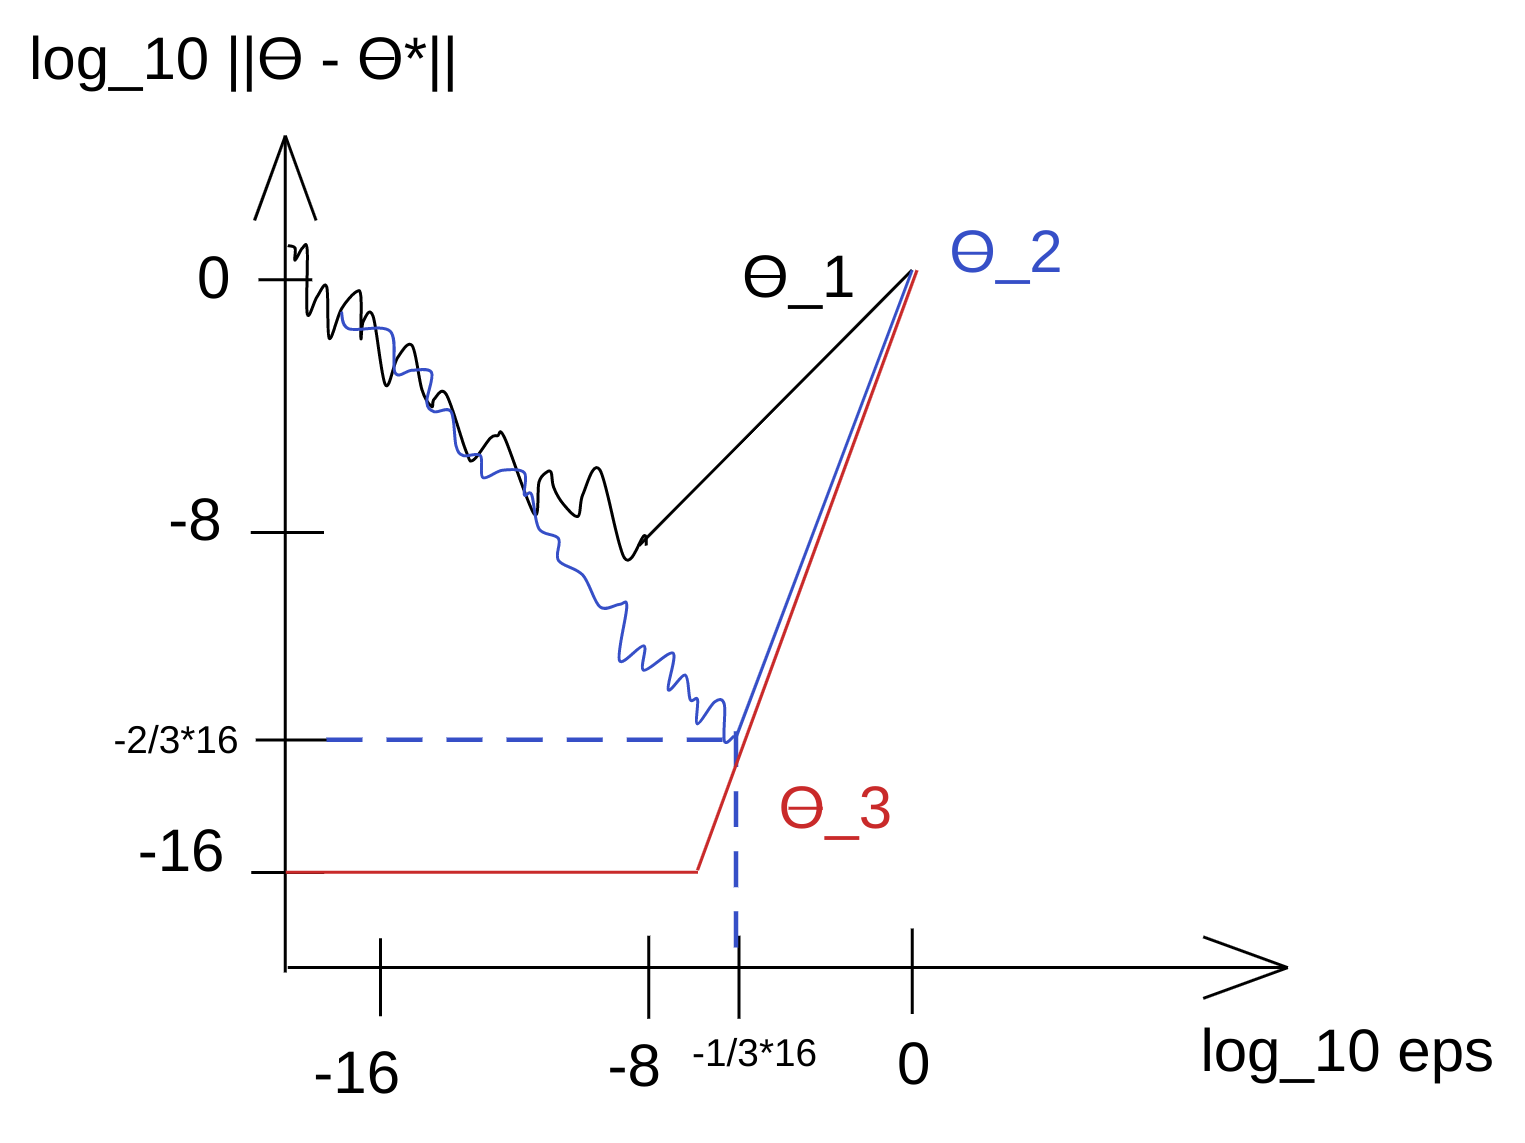
\includegraphics[width=10cm, height=8cm]{images/kir_pic.png}
    \label{ris:im225}
    \caption{Точность при разностном дифференцировании}
\end{figure}
На графике $\Theta_* = \nabla^2 f(x)d$
\\

\textbf{Итого}: 1) способ вычисляет всего 1 градиент, но может получить не такую большую точность. 2) способ считает 2 градиента, но получает лучше точность. 3) способ считает 1 градиент(но из-за перехода к комплексным на самом деле больше), но имеет лучшую сколь угодно низкую точность, применим не ко всем функциям.



    \subsection{Квазиньютоновские методы. Схемы BFGS и L-BFGS. @isadrtdinov}

    Как непосредственно следует из названия, квазиньютоновские методы пытаются вести себя как обычный метод Ньютона. Вспомним, что на каждой итерации метода Ньютона мы решаем систему линейных уравнений (по сути обращаем гессиан), что приводит к сложности итерации $\mathcal{O}(n^3)$. Кроме того, от нас требуется подсчитывать сам гессиан, что может быть нетривиальной задачей для некоторых функций, например, для нейросетей или для логистической регрессии (привет, ТИ!). Все квазиньютоновские методы оперируют градиентом и с помощью него итеративно приближают гессиан функции. Мотивация использовать квазиньютоновские методы очень простая: мы снижаем затраты по времени, но при этом сохраняем суперлинейную скорость сходимости.

Разберем подход, который приводит к квазиньютоновским методам. Вспоминаем про многомерный ряд Тейлора и приближаем нашу гладкую функцию квадратичной моделью:

$$
f(x_k + d_k) \approx \widehat{f}_k(d_k) = f_k + \nabla f_k^T d_k + \frac{1}{2} d_k^T B_k d_k
$$

\noindent
Матрица $B_k$ - симметричная (таков гессиан) и положительно-определенная (это необходимо для выпуклости квадратичной модели $\widehat{f}_k(d_k)$, чтобы функция обладала единственным минимумом). В ванильном методе Ньютона мы используем $B_k = \nabla^2 f(x_k)$, но мы уже договорились, что такой подход нас не устраивает.

Мы хотим найти оптимальное направление, вдоль которого нужно сделать шаг. Приравняв к нулю градиент $\widehat{f}_k(d_k)$, мы получим систему линейных уравнений:

$$
B_k d_k = -\nabla f_k \Leftrightarrow d_k = -B_k \nabla f_k
$$

\noindent
После этого с помощью линейного поиска мы находим длину $\alpha_k$ и делаем шаг спуска:

$$
x_{k + 1} = x_k + \alpha_k d_k
$$

\noindent
Получаем аппроксимацию функции в новой точке:
$$
\widehat{f}_{k + 1}(d) = f_{k+1} + \nabla f_{k + 1}^T d + \frac{1}{2} d^T B_{k + 1} d
$$

Нужно сочинить какие-то разумные требования для матрицы $B_{k + 1}$, чтобы она была похожа на гессиан. Закажем, чтобы градиент функция $\widehat{f}_{k+1}$ совпадал с градиентом исходной функции $f$ в точках $x_k$ и $x_{k+1}$:

$$
\nabla f_k = \nabla f (x_{k+1} - \alpha_k d_k) = \nabla \widehat{f}_{k + 1}(-\alpha_k d_k) = \nabla f_{k+1} - \alpha_k B_{k+1} d_k
$$

$$
\nabla f_{k+1} = \nabla \widehat{f}_{k + 1}(0) = \nabla f_{k+1}
$$

\noindent
Второе уравнение тривиально, а вот из первого можно вывести линейное ограничение на $B_{k+1}$:

$$
B_{k+1} \alpha_k d_k = \nabla f_{k+1} - \nabla f_k
$$

Приняв $s_k = x_{k+1} - x_k = \alpha_k d_k$ и $y_k = \nabla f_{k+1} - \nabla f_k$, получаем ограничение, именуемое \textbf{уравнением секущей}:

$$
B_{k+1} s_k = y_k
$$

\noindent
Это ограничение используется во всех квазиньютоновских методах. При этом, искомая матрица $B_{k+1}$ существует только при условии $s_k^T y_k > 0$. Если функция $f$ сильно выпукла, то это неравенство выполнено для любых векторов $x \ne y$ (пользуемся дифференциальным критерием первого порядка):

$$
\begin{cases}
    f(y) \ge f(x) + \nabla f(x)^T (y - x) + \frac{\mu}{2} \|y - x\|^2 \\
    f(x) \ge f(y) + \nabla f(y)^T (x - y) + \frac{\mu}{2} \|y - x\|^2
\end{cases} \Rightarrow
$$

$$
f(x) + f(y) \ge f(x) + f(y) + \big(\nabla f(x) - \nabla f(y)\big)^T (y - x) + \mu \|y - x\|^2
$$

$$
\big(\nabla f(y) - \nabla f(x)\big)^T (y - x) \ge \mu \|y - x\|^2 > 0
$$

\noindent
Если же функция не является сильно выпуклой, то выполнение неравенство обеспечит (слабое) условие Вульфа, поэтому именно его применяют для линейного поиска в квазиньютоновских алгоритмах.

$$
\nabla f(x_{k+1})^T d_k \ge c_2 \nabla f(x_k) d_k
$$

$$
\big(\nabla f(x_{k+1}) - \nabla f(x_k)\big)^T \alpha_k d_k \ge (c_2 - 1) \alpha_k  \nabla f(x_k) d_k
$$

$$
\big(\nabla f(x_{k+1}) - \nabla f(x_k)\big)^T (x_{k+1} - x_k) \ge (c_2 - 1) \alpha_k \nabla f(x_k) d_k = (< 0) \cdot (> 0) \cdot (< 0) > 0
$$

Все квазиньютоновские методы обновляют матрицу $B_k$ по правилу $B_{k+1} = B_k + U_k$, где $U_k$ - матрица невысокого ранга. Это необходимо для эффективного вычисления обратной матрицы $H_{k + 1} = B_{k+1}^{-1} = \left(B_k + U_k \right)^{-1}$. Конкретный вид матрицы $U_k$ и отличает разные квазиньютоновские методы.

\vspace{6pt}
\textbf{\large SR-1}

SR-1 - это простейший квазиньютоновский метод, назван так за то, что обновляет гессиан симметричной матрицей ранга 1. Формула обновления $B_k$ такая:

$$
B_{k+1} = B_k + \sigma v v^T
$$

\noindent
Здесь $\sigma = +1$ или $-1$, а $\sigma$ и $v$ подбираются так, чтобы выполнялось уравнение секущей. Итоговые формулы для метода такие:

$$
B_{k+1} = B_k + \frac{(y_k - B_k s_k)(y_k - B_k s_k)^T}{(y_k - B_k s_k)^T s_k}
$$

$$
H_{k+1} = H_k + \frac{(s_k - H_k y_k)(s_k - H_k y_k)^T}{(s_k - H_k y_k)^T y_k}
$$

\noindent
У схемы SR-1 есть ряд недостатков: получаемые матрицы могут не быть положительно определенными, а знаменатель порой оказывается очень маленьким, что выражается в численной неусточивойсти. Однако, утверждается, что матрицы в SR-1 хорошо аппроксимируют настоящий гессиан. Со скоростью сходимости здесь сложно. Если методу удается избежать проблем с положительной определенностью и знаменателем, то сходимость суперлинейная. Но зачастую метод ведет себя очень неустойчиво.

\vspace{6pt}
\textbf{\large BFGS}

Матрица $H_{k+1}$, используемая в методе BFGS, является решением следующей оптимизационной задачи (не уверен, что это нужно, но просто забавный факт):

$$
\begin{cases}
    \|H - H_k\|_W \rightarrow \displaystyle\min_{H \in \Sym^n_{++}} \\
    H y_k = s_k
\end{cases}
$$

\noindent
Здесь используется взвешенная норма Фробениуса: $\|A\|_W = \|W^{1/2} A W^{1/2}\|_F$, а в качестве матрицы весов берется любая, удовлетворяющая условию $W s_k = y_k$. Ограничение в системе - это уравнение секущей, записанное через матрицу $H_{k+1}$ $(B_{k+1} s_k = y_k \Leftrightarrow H_{k+1} y_k = s_k)$.

Эта оптимизационная задача имеет единственное решение, которое дает нам формулу для обновления матрицы $H_k$:

$$
H_{k+1} = \left(I_n - \frac{s_k y_k^T}{\langle y_k, s_k \rangle}\right) H_k \left(I_n - \frac{y_k s_k^T}{\langle y_k, s_k \rangle}\right) + \frac{s_k s_k^T}{\langle y_k, s_k \rangle}
$$

\noindent
При этом формула для обновления $B_k$ выглядит так (она не нужна в реализации алгоритма, но ее стоит знать):

$$
B_{k+1} = B_k - \frac{B_k s_k s_k^T B_k}{\langle B_k s_k, s_k \rangle} + \frac{y_k y_k^T}{\langle y_k, s_k \rangle}
$$

С первого взгляда может показаться, что мы не облегчили себе задачу: ведь при пересчете $H_k$ мы перемножаем матрицы, а сложность этой операции все так же $\mathcal{O}(n^3)$. Но если раскрыть скобки в формуле, то все операции в ней упростяться до сложности $\mathcal{O}(n^2)$ (это умножение матрицы на вектор, умножение вектора-столбца на вектор-строку и скалярное произведение):

$$
H_{k+1} = H_k + \frac{\left(y_k^T s_k + y_k^T H_k y_k\right) s_k s_k^T}{\langle y_k, s_k \rangle^2} - \frac{s_k y_k^T H_k + H_k y_k s_k^T}{\langle y_k, s_k \rangle}
$$

Осталось договориться о выборе начального приближения $H_0$. На этот случай нет универсального варианта, и обычно принимают либо $H_0 = I_n$, либо можно оценить гессиан в точке $x_0$ через конечные разности и обратить его.

Общая схема метода выглядит так:

\begin{algorithm}[H]
    \begin{algorithmic}[1]
        \Procedure{BFGS}{$f, x_0, H_0, \varepsilon$}
            \For{$k=0, 1, 2, ...$}
                \State $d_k \gets -H_k \nabla f_k$
                \State $\alpha_k \gets \textsc{LineSearch}(f, x_k, d_k)$
                \State $x_{k+1} \gets x_k + \alpha_k d_k$
                \State $s_k \gets x_{k+1} - x_k$
                \State $y_k \gets \nabla f_{k+1} - \nabla f_k$
                \State $H_{k+1} \gets \textsc{UpdateInversedHess}(H_k, s_k, y_k)$
                \If{$\|\nabla f_{k+1}\| < \varepsilon$}
                    \textbf{break}
                \EndIf
            \EndFor
            \State \Return $x_k$
        \EndProcedure
    \end{algorithmic}
\end{algorithm}

К сожалению, ничто в этом мире не идеально, даже метод BFGS. Нам удалось сократить время итерации до $\mathcal{O}(n^2)$, но нам все еще нужно хранить плотную матрицу $H_k$, и это обеспечивает затраты на память $\mathcal{O}(n^2)$, что не всегда возможно. Тем не менее, метод BFGS имеет суперлинейную сходимость, что делает его популярным на практике.

\vspace{6pt}
\textbf{\large L-BFGS}

Метод L-BFGS - это модификация стандартного BFGS, которая позволяет сэкономить память и не хранить гессиан целиком. Все что от нас требуется - уметь умножать гессиан на произвольный вектор. Для этого метод поддерживает историю $\mathcal{H}_k = \{(s_{k - i}, y_{k - i})\}_{i=1}^l$ из последних $l$ пар векторов. Вводится начальное приближение $H_{k-l}$:

$$
H_{k-l} = \gamma_0^{(k)} I_n, \text{ где } \gamma_0^{(k)} = \frac{\langle y_{k-1}, s_{k-1} \rangle}{\langle y_{k-1}, y_{k-1} \rangle}
$$

Новое приближение $H_k$ получается из $H_{k-l}$ путем $l$-кратного применения формулы из BFGS. Однако существует рекурсивная процедура, позволяющую подсчитывать произведение $d_k = -H_k \nabla f_k$ без формирования матриц в памяти. Выглядит она так:

\begin{algorithm}[H]
    \begin{algorithmic}[1]
        \Procedure{Multiply}{$v, \mathcal{H}, \gamma_0$}
            \If{$\mathcal{H}$ = \O}
                \Return $\gamma_0 v$
            \EndIf
            \State $(s, y) \gets \text{ последняя пара из } \mathcal{H}$
            \State $\mathcal{H}' \gets \mathcal{H} \text{ без последней пары}$
            \State $v' \gets v - \frac{\langle s, v \rangle}{\langle y, s \rangle} y$
            \State $z \gets \textsc{Multiply}(v', \mathcal{H}', \gamma_0)$
            \State \Return $z + \frac{\langle s, v \rangle - \langle y, z \rangle}{\langle y, s \rangle} s$
        \EndProcedure

        \State $\gamma_0^{(k)} = \frac{\langle y_{k-1}, s_{k-1} \rangle}{\langle y_{k-1}, y_{k-1} \rangle}$
        \State $d_k = -\textsc{Multiply}(\nabla f_k, \mathcal{H}_k, \gamma_0^{(k)})$
    \end{algorithmic}
\end{algorithm}

Таким образом, сложность итерации для вычисления направления $d_k$ получается $\mathcal{O}(nl)$ (без учета сложности вычисления функции и градиента), а необходимая память для поддержания истории - $\mathcal{O}(nl)$. Типичное значение параметра размера истории $l=10$ (при $k < l$ история $\mathcal{H}_k$ состоит только из $k$ пар). Заметим, что при $l=\infty$ мы в точности получаем метод BFGS, а при $l=0$ - обычный градиентный спуск. На практике L-BFGS показывает себя лучше методов оптимизации первого порядка, хоть и не обладает суперлинейной сходимостью (гарантирована только линейная скорость сходимости).


    \subsection{Стандартные классы выпуклых задач: линейное программирование (LP), коническое квадратичное программирование (CQP/SOCP), полуопределенное программирование (SDP). Примеры задач для каждого из классов. Сводимость. L/CQ/SD-представимые множества и функции.}

    Все написано \href{https://drive.google.com/file/d/1GXgex6RrwWv_wGBh4oYLpUcWD5-Yc3UM/view}{здесь}.

    \subsection{Симплекс-метод для решения задачи линейного программирования (в версии revised simplex method). Примеры сведения задачи линейного программирования к канонической форме. @elvarid}

    Чтобы понимать билет, вначале обратитесь к вопросам 1.12 и 1.13

 \subsubsection{Примеры сведения задачи линейного программирования к канонической форме}

 Смотреть пункт 1.12

 \subsubsection{Симплекс-метод для решения задачи линейного программирования (в версии revised simplex method)}

 \textbf{Определение:} $x$ - угловая точка множества $F$, если $\not\exists y, z \in F, y,z \neq x, \alpha \in (0, 1) : x = \alpha y + (1 - \alpha) z$


 \textbf{Утверждение:} $x$ - угловая точка множества $\{ x | Ax = b, x \ge 0 \}  \Leftrightarrow \exists B, N : \{1, 2, ..., n\} = B \cup N , |B| = p, |N| = n - p, x_N = 0, A_B = [A_{.,i}]_{i\in B} \in \mathbb{R}^{p x p} $ - невырожденная


 \textit{Ремарка - $B$ от слова базис}


 $Ax= b = A_B x_B + A_N x_N, x_B \in \mathbb{R}^{p} , x_N \in \mathbb{R}^{n - p}$, знаем, что $x_N = 0 \Rightarrow x_B = A_b^{-1} * b \ge 0$

 \textit{На лекции было сказано что факт доказывается тривиально}
 \qed

 Перестановка одной координаты в множествах $B$ и $N$ соответствует переходу к соседней угловой точке.


 Запишем вновь нашу задачу линейного программирования и условия ККТ чтобы пояснить как находить угловую точку.

 Задача условной оптимизации:
\[
    \begin{cases}
         c^Tx \to \underset{x}{min}, x \in \mathbb{R}^n\\
         Ax = b,\\
         x \ge 0\\
    \end{cases}
\]

Функция Лагранжа:
\[
    L(x, \lambda, \mu) = c^T x - \lambda^T x + \mu^T(Ax - b)
\]

Запишем условия ККТ:
\[
    \begin{cases}
         \nabla_x L(x, \lambda, \mu) = c - \lambda + A^T \mu = 0,\\
         Ax = b,\\
         \lambda \ge 0\\
         \lambda_i x_i = 0, \: i=1,\dots, n
    \end{cases}
\]


$x$ - угловая точка, $x_N = 0, x_B = A_b^{-1}b \ge 0$ - то есть есть такое разбиение. Давайсте восстановим значения $\lambda $ и $\mu$ чтобы ККТ были выполнены.

$\lambda_B = 0$ - тогда произведение для всех индексов в ККТ будет равно нулю. Запишем следующее: $A^T\mu + c = \lambda$.  Рассмотрим в этом уравнение подмножество, соответствующее $B$: $A_B^T \mu + c_B = \lambda_b = 0 \Rightarrow \mu = -A_b^{-T} c_B$ Таким образом мы восстановили $\mu$.  С этим знанием мы можем найти $\lambda_N$: $A_N^T \mu + c_N = \lambda_N \Rightarrow \lambda_N = c_N - A_N^T A_B^{-T} c_B = c_N - (A_B^{-1} A_N)^T c_B$. Таким образом мы удовлетворили всем условия ККТ, кроме третьего условия, с которым еще надо повозиться.

Если уже $\lambda_N \ge 0 \Rightarrow x - $ решение.

Если это не выполнено, то ситуация следующая:
$\exists q \in N : \lambda_q < 0$ и надо идти в другую угловую точку.

Теперь неформально можно описать шаг симплекс-метода : увеличиваем $x_q$ до тех пор, пока какой-то из $(x_B)_i$ не станет равен нулю. Это и будет означать переходу в соседнюю угловую точку.

 Распишем в виде формул.

 Изначально есть $x: Ax = b, x_N = 0$. Вместо этой точки строим точку $x^+ : x_i^+ = 0, i\in N\backslash \{q\}$. Тогда получается следующее: $$
 Ax^+ = b = A_B x_B^+ + A_q x_q^+ = A_B x_B
 $$

Поделим это выражение на невырожденную $A^{-1}$:
$$
x_B^+ = x_B - A_B^{-1} A_q x_q^+
$$

$A_B^{-1} A_q$ это какой-то вектор $d$ размера $p$. $x_q^+$ это число. Тогда получается:
$$
x_B^+ = x_B - d x_q^+ \ge 0
$$

Если все компоненты вектора $d$ меньше либо равны $0$ то решений не будет. Если же найдутся $\exists j : d_j > 0$, то переход в ноль какой-то компоненте будет соответствовать следующему:

$$
(x_B)_j - d_j x_q^+ = 0 \Rightarrow x_q^+ = \frac{(x_B)_j}{d_j}
$$

Если же таких $j$ несколько, то $x_q^+ = \underset{j:d_j > 0}{min} \frac{(x_B)_j}{d_j}$
 Осталось только перекинуть один индекс из множества $B$ в $N$:

 $$
 B = B \cup \{q\} \backslash \{j\} \\
 N = N \backslash \{q\} \cup \{j\}
 $$

 Вот так выглядит шаг симплекс-метода. Давайте докажем, что действительно на каждом шаге есть прогресс.

 \textbf{Утверждение:} На каждом шаге симплекс-метода целевая функция уменьшается

 \noindent

 \textit{Доказательство:}
 $$ c^T x^+ = c_B^T X_B^+ + c_q x_q^+ = c_B^T (x_B - d x_q^+) + c_q x_q^+ = c_B^T x_B + x_q^+(c_q - c_B^T d)$$

 Рассмотрим $c_B^T d$. Это выражение равно $c_b^T A_B^{-1} A_q$, а ранее мы установили, что это равно $- \mu^T A_q = - (\lambda_q - c_q)$

 Подставим этот результат в предыдущее выражение:

 $$
 c_B^T x_B + x_q^+(c_q - c_B^T d) = c^T x + x_q^+(c_q + \lambda_q - c_q) = c^T x + \lambda_q x_q^+
 $$

 Если мы посмотри на знак последнего слагаемого, то он будет отрицательный, так как уже известно, что $\lambda_q < 0$, мы ее такой выбрали, а $x_q^+$ в свою очередь строго больше нуля (так как мы в ту сторону двигаем)

 Значит $c^T x + \lambda_q x_q^+ < c^T x$

 Таким образом значение целевой функции уменьшается на каждом шаге метода. \qed

 Теперь формально опишем один шаг симплекс-метода.

\textbf{Шаг симплекс-метода:}
\begin{algorithm}[H]
    \begin{algorithmic}[1]
        \Procedure{Revised simplex method step}{$x: x_N = 0, x_B = A_b^{-1} b \ge 0$}
        \State Решить СЛАУ $A_B^T \mu = - c_B$
        \State $\lambda_N \gets c_N + A_N^T \mu$
        \State Если $\lambda_N \ge 0,$ то СТОП (найдено оптимальное решение)
        \State Выбрать $q\in N, \lambda_q < 0$
        \State Решить СЛАУ $A_B d = A_q$
        \State Если $d \le 0,$ то СТОП (решения не существует)
        \State $x_q^+ \gets \underset{i : d_i > 0}{min} \frac{(x_B)_i}{d_i}$
        \State $j \gets \underset{i : d_i > 0}{argmin} \frac{(x_B)_i}{d_i}$
        \State $x_B^+ \gets x_b - d x_q^+$
        \State $x_N^+ \gets (0, 0, \dots, x_q^+, 0, \dots, 0)$
        \State $B \gets B \cup \{q\} \backslash \{j\}$
        \State $N \gets N \backslash \{q\} \cup \{j\}$
        \State \Return $x$
        \EndProcedure
    \end{algorithmic}
\end{algorithm}

Прокомментируем еще раз алгоритм. Сначала по заданной точке мы находим $\mu$ и $\lambda$. Собственно изначально мы решаем СЛАУ относительно $\mu$, и с помощью $\mu$ находим $\lambda$. Если все $\lambda$ неотрицательные, то мы удовлетворили условиям ККТ и у нас есть решение, поэтому мы останавливаемся. Если же условие не выполнено, то мы выбираем какую-то компоненту $\lambda_q$ меньше нуля и дальше начинаем двигать точку $x_q$ на вектор $d$. Вектор $d$ мы находим через решение СЛАУ. Если все компоненты этого вектора неположительные, то это означает что целевую функцию можно увести в минус бесконечность, тогда решений не существует. Если же хотя бы один $d$ положительный, то тогда мы совершаем сдвиг согласно написанным формулам.
И в конце перекидываем индексы между $B$ и $N$.

По итогу что мы имеем метод, который сходится за конечное число шагов (благодаря доказанному выше утверждению про уменьшение целевой функции на каждом шаге). Однако, справедлива будет для общего случая следующая оценка на число шагов - $C_n^p$(число сочетаний) по построению метода. На практике эта сложность практически неактуальна (даже теоретический пример для такой сложности предъявили не сразу после создания метода), часто метод находит оптимальную точку за линейное время от $p$.

Стоит обсудить еще следующую особенность симплекс-метода. Как видно по алгоритму, здесь нет какого-то понятия вроде эпсилон-точности, как в предыдущих рассмотренных методах. Либо мы в итоге приходим в оптимум, либо нет. Это связано с особенностью хождения по угловым точкам. В какой-то момент мы можем пройти очень маленькое расстояние, так как две угловые точки находятся очень близко друг к другу, но это не значит, что оптимум близко, хотя изменение целевой функции будет минимальным. Из-за этой причины нет смысла в каком-то заранее задаваемом параметре точности.

Информацию далее для сдачи экзамена учить не надо, но если вы будете это знать, то это будет полезно (информация с консультации)

\textbf{Возникающие проблемы при использовании.}
\begin{itemize}

    \item На каждом шаге у матрицы $A_B$ меняется только один столбец, поэтому в некоторых реализациях хранится только $LU$ разложение, в котором изменения происходят с помощью специальных алгоритмов.

    \item Момент связанный с выбором компоненты $q$. Изначально была стратегия $q^* = \underset{q}{argmin} \lambda_q $. Данная стратегия обоснована анализом уменьшения функции на итерации метода. На практике в этом месте это было бы слишком дорого, поэтому в этом моменте возникают различные эвристики которые хорошо выбирают  $q$.

    \item Момент связанный с вырожденными точками. Угловая точка называется вырожденной, если какая-то или несколько из компонент из $B$ равны нулю. В таком случае $x_q^+$ двигать за пределы множества нельзя, и эта компонента будет равна $0$. Тогда изменение целевой функции не уменьшится, метод может даже зациклиться между несколькими вырожденными точками. В таком случае надо вставить какой-то АНТИЦИКЛИН (что-то вроде добавления нормального шума к вектору $b$ из $Ax = b$.

    \item Момент связанный с выбором начальной угловой точки. Не всегда очевидно как выбрать начальную точку, один из возможных способов решения это так называемый метод "первый фазы". Он заключается в формировании какой-то специальной задачи, про которую известно что ее решение будет содержать какую-то угловую точку нашего изначального множества ($Ax = b$), и для этой задачи мы без проблем умеем выбирать начальную угловую точку. То есть первую фазу мы решаем с помощью симплекс-метода, получаем начальную точку и решаем уже с этой начальной точкой нашу задачу, так называемая вторая фаза.

\end{itemize}

    \subsection{Метод Ньютона и логарифмических барьеров для выпуклых задач условной оптимизации с ограничениями вида равенств и неравенств. @arinaruck}

    \textbf{Что будет в билете:} Сначала научимся решать задачу условной оптимизации с ограничениями только вида равенств, потом введем барьерную функцию для ограничений вида неравенств и приведем искодную задачу к эквивалентному виду только с равенствами в ограничениях

\bigskip

Задача с ограничениями только вида равенств:
\[
\begin{cases}
f(x) \to min_x, \ x \in D \subseteq \mathbb{R}^n, \ f \text{вып} \in C^{2} \\
Ax = b, A \in \mathbb{R}^{p \times n}, p < n, \ rank A = p
\end{cases}
\]

$F = \{ x \in D : Ax = b \}$

\bigskip


$x_{k+1} = x_k + \alpha_k d_k$, $d_k$ направление спуска для f

Хотим сохранять допустимость, то есть чтобы все $x_i \in F$ : $x_0 \in F \to x_1 \in F \to \dots $

$f(x_k + d) \approx m_k(d) = f(x_k) + \nabla f(x_k)^Td + \dfrac{1}{2} d^TB_k d \to min_d, \ B_k \in S_{++}^n $
$A(x_k + d) = b$

Чтобы сохранить допустимость решаем задачу QP:

\[
\begin{cases}
 f(x_k) + \nabla f(x_k)^Td + \dfrac{1}{2} d^TB_k d \to min_d \\
 Ad = 0
\end{cases}
\]

Если $B_k = I$ получим метод проекции градиента

\[\begin{cases}
m_k(d) = f(x_k) + \nabla f(x_k)^Td + \dfrac{1}{2} d^T d  = \dfrac{1}{2} \| d + \nabla f(x_k) \|^2  + const \to min_d\\
Ad = 0
\end{cases}
\ \implies \ d = pr_{Ad = 0}(- \nabla f(x_k))
\]


Если $B_k = \nabla^2 f(x_k)$

\[\begin{cases}
m_k(d) = f(x_k) + \nabla f(x_k)^Td + \dfrac{1}{2} d^T \nabla^2 f(x_k)d  = \dfrac{1}{2} \| d +[ \nabla^2 f(x_k)]^{-1} \nabla f(x_k) \|^2_{\nabla^2 f(x_k)}  + const \to min_d\\
Ad = 0
\end{cases}
\]

$\| x \|^2_{B} = x^TBx, \ B \in S_{++}^n$

Уже нельзя так просто взять проекцию, так как измененная норма

\bigskip

Запишем Лагранжиан для функции по d:


$L(d, \mu) =  f(x_k) + \nabla f(x_k)^Td + \dfrac{1}{2} d^TB_k d + \mu (Ad)$


Выпишем ККТ:

\[
\begin{cases}
\nabla_{d} L(d, \mu) = \nabla f(x_k) + B_kd + A^T\mu = 0 \\
Ad = 0
\end{cases}
\]

Получили СЛАУ относительно $d, \ \mu$

Перепишем в блочном виде:

\[
\begin{bmatrix}
B_k & A^T \\
A & 0
\end{bmatrix}
 \cdot
  \begin{bmatrix}
  d \\
  \mu
 \end{bmatrix} =
  \begin{bmatrix}
-\nabla f(x_k) \\
0
\end{bmatrix} ,
d \in \mathbb{R}^n, \ \mu \in \mathbb{R}^p
\]

Обозначим

\[
K =
\begin{bmatrix}
	B_k & A^T \\
	A & 0
\end{bmatrix}
\]

$inertia(K) = (n_{+1}, n_{-1}, n_0)$ —  количество положительных, отрицательных и нулевых собственных значений K

\bigskip

Если $B_k \succ 0, \ rank A = p \ \implies inertia(K) = (n, p ,0)$, так как нет нулевых собственных значений, матрица К невырожденная, тогда решение исходной системы единственно.

К симметричная и не положительно определенная, если есть хотя бы одно ограничение вида равенства. Можем решать систему, например, с помощью LDL (если не очень большая), или метода типа CG (Крыловского вида), если очень.

\bigskip

$x_{k+1} = x_k + \alpha_k d_k$

\medskip

Для корректности нужно:

1) $x_{k+1} \in F$ —  точка допустима

2) $\nabla f(x_k)^T d_k < 0$ —   $d_k$ направление спуска

\bigskip

Проверим:

1) $x_{k+1} \in F \  \Leftrightarrow x_{k+1} \in \{x \in D: Ax = b \}$

$Ax_{k+1} = A(x_k + \alpha_k d_k) = Ax_k + \alpha_k Ad_k = b$

Должны прогарантировать, что возьмем $\alpha_k$, которая не выведет нас из домена D, для этого можем, например, выполнить поиск следующим образом

 \begin{algorithm}[H]
	\begin{algorithmic}[1]
		\Procedure{$\alpha_{max}$}{$\alpha_0 = 1$}
		\For{$k=0, 1, 2, ...$}
		\If{$x_{k} + \alpha_k d_k \in D$} \textbf{break}
		\EndIf
		\State $\alpha_{k+1} \gets \alpha_k / 2 $
		\EndFor
		\State \Return $\alpha_k$
		\EndProcedure
	\end{algorithmic}
\end{algorithm}


Из $a_k$ будем начинать одномерный поиск для условий Армихо/Вульфа (для простых доменов можем также находить аналитически)

\bigskip

2) $\nabla f(x_k)^Td_k = d_k^T(-B_kd - \mu_k A^T) = -d_k^T B_k d - \mu_k (Ad_k)^T = -d_k^T B_k d  < 0$

То есть $d_k$ является направлением скуска

\bigskip

Критерий останова:

$\|\nabla_x L(x_{k+1}, \mu)\| = \|\nabla f(x_{k+1}) + A^T\mu_{k+1} \| < \varepsilon$

Скорость сходимости полностью наследует скорость сходимости для безусловного случая (т. е. зависит только от выбора $B_k$ в приближении)

\bigskip

Теперь перейдем к случаю, когда ограничения могут быть не только вида равенств но и неравенств


\[
\begin{cases}
f(x) \to min_x, \ x \in D \subseteq \mathbb{R}^n, \ f, g_i \text{вып} \in C^{2} \\
g_i(x) \leqslant 0, i = 1,  \dots, m\\
Ax = b, A \in \mathbb{R}^{p \times n}, p < n, \ rank A = p
\end{cases}
\]

Пусть выполнено условие Слейтера, то есть $\exists \hat{x} : A\hat{x} = b,  \ g_i(\hat{x}) < 0 \ \forall i$

Введем индикаторную функцию

\[I(u) = \begin{cases}
0, u \leqslant 0 \\
+\infty, \text{иначе}
\end{cases}
\]

Тогда можем переписать исходную задачу в виде

\[
\begin{cases}
f(x)  + \sum_{i=1}^{m} I(g_i(x))\to min_x \\
Ax = b, A \in \mathbb{R}^{p \times n}, p < n, \ rank A = p
\end{cases}
\]

Хотелось бы применить метод, который описали до этого, но индикатор не гладкий, хотим его сгладить

$I_{\tau}(u) = -\dfrac{1}{\tau} log(-u), \ \tau > 0$                                          —  логарифмический барьер

$I_{\tau}(u) \underset{\tau \to + \infty}{\to} I(u)$

Тогда перейдем к

$$
\begin{cases}
f(x)  - \dfrac{1}{\tau} \sum_{i=1}^{m} log(-g_i(x))\to min_x \\
Ax = b, A \in \mathbb{R}^{p \times n}, p < n, \ rank A = p
\end{cases}
$$

$D = \{x : g_i(x) < 0\}$
выпуклая гладкая задача оптимизации


$$$$

Рассмотрим $\{\hat{x}(\tau), \hat{\mu}(\tau)| \tau > 0 \}$   —  центральный путь

Пример: (См. рисунок)

\[
\begin{cases}
c^Tx \to min_x\\
Ax \leqslant b
\end{cases}
\]

$F_{\tau}(x) = c^Tx  - \dfrac{1}{\tau}\sum_{i=1}^m log(-a_i^Tx + b) \to min_x$

$\dfrac{1}{\tau}\sum_{i=1}^m log(-a_i^Tx + b)  = \phi_{\tau}(\hat{x}(\tau)) $

$\nabla_x F_{\tau} = c + \nabla_x \phi_{\tau}(\hat{x}(\tau)) = 0  \implies  \nabla_x \phi_{\tau}(\hat{x}(\tau)) = - c$

Будем идти по центральному пути, начиная из центральной точки, постепенно увеличивая $\tau$, повышая "вес" $c^Tx$

Чем больше $\tau$, тем ближе линия уровня к границе


\begin{figure}[H]
        \minipage{0.45\textwidth}
        \centering
        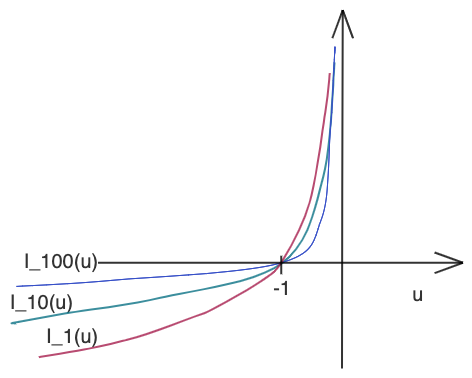
\includegraphics[scale=0.45]{images/ind_pic.png}
        \label{}
        \caption{$I_{\tau}(u)$функции.}
        \endminipage\hfill
        \minipage{0.45\textwidth}
        \centering
        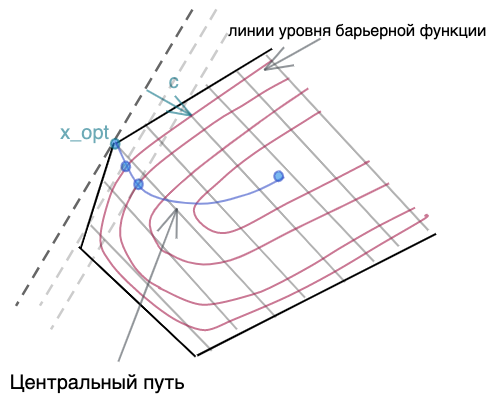
\includegraphics[scale=0.45]{images/path_pic.png}
        \label{}
        \caption{Центральный путь для примера.}
        \endminipage\hfill
\end{figure}



$L_{\tau}(x, \mu) = f(x) - \dfrac{1}{\tau} \sum_{i=1}^m log(-g_i(x)) + \mu^T(Ax - b)$

$\nabla_x L_{\tau}(\hat{x}, \hat{\mu}) = \nabla_x f(\hat{x}) + \dfrac{1}{\tau} \sum_{i=1}^m \dfrac{-\nabla_x g_i(\hat{x})}{g_i(\hat{x})} + A^T\hat{\mu} = 0$

При этом для исходной задачи:

$L_{\tau}(x, \mu, \lambda) = f(x) + \sum_{i=1}^m \lambda_i g_i(x) + \mu^T(Ax - b)$

$\nabla_x L_{\tau}(\hat{x}, \hat{\mu}, \hat{\lambda }) = \nabla_x f(\hat{x}) +
 \sum_{i=1}^m \nabla_x \hat{\lambda_i}g_i(\hat{x}) + A^T\hat{\mu} = 0$

 Тогда введем обозначение: $\hat{\lambda_i} = \dfrac{-1}{\tau g_i(\hat{x})}$


 Для $(\hat{x}(\tau), \hat{\mu}(\tau), \hat{\lambda}(\tau)):$

 \[
 \begin{cases}
 \nabla_x  L_{\tau}(\hat{x}, \hat{\mu}, \hat{\lambda }) = 0 \\
 A\hat{x} = b \\
\hat{ \lambda_i}  > 0 \ \forall i=1, \dots, m \\
\hat{\lambda_i} g_i(\hat{x}) = -\dfrac{1}{\tau} \ \forall i=1, \dots, m
\end{cases}
 \]


При $\tau \to + \infty$ $(\hat{x}(\tau), \hat{\mu}(\tau), \hat{\lambda}(\tau))$ удовлетворяет ККТ для исходной задачи

Введем двойственную функцию:

$g(\lambda, \mu) = inf_x L(x, \mu, \lambda)$

$g(\lambda, \mu) \leqslant f_{opt} \ \forall \mu, \forall \lambda > 0$

$g(\hat{\lambda}, \hat{\mu}) = L(\hat{x}, \hat{\mu}, \hat{\lambda}) \leqslant f_{opt}$

$f(\hat{x}) - f_{opt} \leqslant f(\hat{x}) - L(\hat{x}, \hat{\mu}, \hat{\lambda}) = f(\hat{x}) - f(\hat{x}) + \sum_{i=1}^m \hat{\lambda_i} g_i(\hat{x}) + \hat{\mu}^T(A\hat{x} - b)  = \dfrac{m}{\tau}$

$ \ (\hat{x} \text{ допустимое } \implies A\hat{x} = b)$

$\dfrac{m}{\tau} = \varepsilon, \ \tau = \dfrac{\varepsilon}{m}$

На практике постепенно увеличиваем $\tau$

\bigskip

Приведем общую схему метода:

\begin{algorithm}[H]
	\begin{algorithmic}[1]
		\Procedure{$logarithmic barrier$}{$x_0 \in D, Ax_0 = b, g_i(x_0) < 0 \ \forall i, \varepsilon, \tau_0, \nu > 1$}
		\For{$k=0, 1, 2, ...$}
		\State найти $\hat{x}(\tau_k)$ решение задачи
		$$ \begin{cases} f(x) - \dfrac{1}{\tau_k}\sum_i log(-g_i(x)) \to min_x \\ Ax=b \end{cases}$$
		с помощью метода Ньютона из начального приближения $x_k$
		\State $x_{k+1} \gets \hat{x}(\tau_k)$
		\If{$\dfrac{m}{\tau_k} \leqslant \varepsilon$} \textbf{break}
		\EndIf
		\State $\tau_{k+1} \gets min\left(\dfrac{m}{\varepsilon}, \tau_k \cdot \nu \right)$
		\EndFor
		\State \Return $\alpha_k$
		\EndProcedure
	\end{algorithmic}
\end{algorithm}

$\nu$ отвечает за трейдоф внешних и внутренних итераций: чем больше $\nu$, тем быстрее дойдем то $\tau_k = \dfrac{m}{\varepsilon}$, тем меньше будет внешних итераций, но тем хуже будет стартовая точка $x_k$, то есть тем больше внутренних итераций.

В качестве $x_0$ необходимо подать внутреннюю точку, иногда ее поиск довольно сложный, тогда нужно воспользоваться методом первой фазы (как в симплекс-методе)


    \subsection{Субградиентный метод для негладких задач оптимизации. Различные способы выбора длины шага. Субдифференциальное исчисление, примеры вычисления субдифференциалов. @sergevkim}

    \textit{Возможно, один из самых простых билетов} \\

Хотим придумать что-то для функции, которая будет дифференцируемой не в каждой точке. Решение - коль скоро мы не можем подсчитать сам дифференциал, можно подсчитать в точке какой-нибудь его аналог. Спойлер: этот аналог мы будем называть субдифференциалом. \\

\textbf{Definition 1}

Пусть выполнено, что $\forall x \exists s: F(x) \geq F(x_0) + s^T (x - x_0)$

Тогда вектор $s^T$ будем называть субградиентом функции $F$ в точке $x_0$ \\

\textbf{Definition 2}

${s: \forall x \exists s: F(x) \geq F(x_0) + s^T (x - x_0)}$

Множество всех субградиентов в точке $x_0$ - субдифференциал, обозначение $\partial F(x_0)$ \\

\textbf{Утверждение 0}. Если функция дифференцируема в точке $x_0$, то субдифференциал будет состоять из единственного вектор - градиента в этой точке $x_0$

\textbf{Утверждение 1}. Субдифференциал - выпуклое множество

Доказывается по определению субдифференциала. Выписываем два определения субдифференциала и складываем неравенства с коэффициентами $\alpha$ и $(1-\alpha)$

\textbf{Утверждение 2}. Необходимое условие минимума в точке $x_0$ аналогично дифференцируемому случаю, только теперь надо проверять, что $0 \in \partial F(x_0)$. Утверждение 1 позволяет решать задачу необходимого условия это геометрически \\

Сам шаг метода звучит просто: это градиентный метод, только вместо градиента в точке берём какой-нибудь субградиент из субдифференциала (при этом по Утверждению 0 этот "какой-нибудь" субградиент будет в точности совпадать с градиентом).

Проблема: мы теперь не можем использовать правило Армихо/Вульфа, т.к. существуют примеры того, что двигаясь вдоль антисубградиента мы будем увеличивать функцию (в видосике он приводит пример того, что линии уровня из себя представляют сплющенные ромбики, задача задаётся формулой $F(x_1, x_2) = |x_1| + \gamma * |x_2| \to min$).

Альтернативные способ задания такой последовательности:

1) $\alpha_k = \alpha_0$ - если мы возьмём константную длину шага, метод сходиться не будет вообще

2) $\alpha_k = \cfrac{\alpha_0}{||z_k||}$ - делим на норму субградиента. Будем ближе к оптимуму, но сходимости всё ещё нет

3) \{$\alpha_k$\} - выбрать такую последовательность, что $\sum_{i = 0}^{\infty} \alpha_i = \infty$, однако $\sum_{i = 0}^{\infty} \alpha_i^2 < \infty$

Пример: $\alpha_k = \alpha_0 / \sqrt{k + 1}$ или такая последовательность, которая сходится к нулю, но не очень быстро \\

Критерий останова: его нет. Просто идём максимальное количество итераций. В памяти храним лучшую точку, так как метод не гарантирует сходимости к минимуму.

Скорость сходимости - $O(\cfrac{1}{\sqrt{k}})$

Примеры субдифференциального исчисления лучше всего смотреть в семинарской записи, там хорошо написано: \href{https://drive.google.com/file/d/175GWh8qsMg6rVO_xkjDvWbmRG_ALzIbm/view}{Примеры}


    \subsection{Проксимальный градиентный метод для задачи композитной оптимизации. Примеры вычисления проксимальных операторов. @poly\_nomial}

    \textbf{Проксимальнй градиентный метод для задачи композитной оптимизации}:\\
В субградиентном методе ранее обсуждалось, что выпуклые но негладкие функции общего вида (т.е. они не в каждой точке дифференцируемые), оптимизировать довольно сложно. Поэтому данный метод переходит от общего вида выпуклых негладких функций к конкретному \textbf{композитному виду функции}, который и оптимизирует.\\

$F(x)=f(x)+h(x)$~-~композитная функция, где $f(x)$~-~её выпуклая, непрерывная и непрерывная по 1 производной часть ($f \in C; f \in C^1$), а $h(x)$~-~выпуклая, непрерывная ($h(x) \in C$), но $h \not\in С^1$. Также функция $h(x)$~-~должна быть простой. Т.е. проксимальный оператор должен легко вычислятся (о нем ниже).\\

Для показа работы проксимального метода будем использовать пример, где $f(x)$~-~просто подходящая функция по всем трем параметрам, а $h(x)=\lambda ||x||_1$. Тогда $f(x)$~-~будет представлять из себя сепарабельную часть функции, также определим, что $f \in C^{1,1}_L$(т.е. у нее на производной есть какое-то ограниение липшица). Далее распишем $F(x)$ как
$$
F(x)=f(x)+h(x) \leq m_k(x)=f(x_k)+\nabla f(x_k)^T(x-x_k)+\frac{L}{2}||x-x_k||^2+h(x) \to \underset{x}{\min}
$$
С негладкой часть пока ничего не сделали, гладкую же расписали через ур-е касательной и канстанту липшица. Дальше выдилим отдельно все слагаемые, зависящие от $x$:
$$
m_k(x)=\frac{L}{2}(x^Tx-2x^Tx_k+\frac{2}{L}\nabla f(x_k)^Tx)+h(x)+const=\frac{L}{2}||x-(x_k-\frac{1}{L}\nabla f(x_k))||^2_2+h(x)+const \to \underset{x}{\min}
$$
$$
\frac{1}{2}||x-(x_k-\frac{1}{L}\nabla f(x_k))||^2_2+\frac{1}{L}h(x) \to \underset{x}{\min}
$$
Далее как раз введем понятие проксимального оператора:\\
$$
prox_h(x):=~\underset{y}{\argmin}\left[\frac{1}{2}||y-x||^2+h(y)\right]
$$
Тогда через этот оператор можно явно показать
$$
\underset{x}{\argmin}m_k(x)=prox_{\frac{1}{L}h}(x_k-\frac{1}{L}\nabla f(x_k))
$$
Это по факту и есть шаг проксимального градиентного метода. Дальше покажем примеры вычисления проксимального оператора:\\
1)~$h(x) \equiv 0 \to prox_h(x):=\underset{y}{\argmin} \frac{1}{2}||y-x||^2 \to x=x$\\
2)~С-вып.; $h(x)=I_c(x)=\begin{cases}
0,~x \in C\\
+\infty,~x \notin C
\end{cases}$\\
В этом примере $I_c(x)$~-~индикаторная функция множества.\\
$\underset{x}{\min}F(x)=\underset{x}{\min}(f(x)+I_c(x))\equiv \underset{x \in C}{\min}f(x)$\\
Тогда $prox_h(x)=\underset{y \in C}{\argmin}\frac{1}{2}||y-x||^2=pr_c(x)$\\
В этом примере важно то, что теория проксимального оператора может применяться не только к выпуклой и непрерывной функции $h(x)$, но и к замкнутой, как в случае с индикаторной функцией.\\
3)~$h(x)=\lambda ||x||_1$~-~наш пациент.
$$
prox_{\lambda ||*||_1}(x)=\underset{y}{\argmin}\left( \frac{1}{2}||y-x||^2+\lambda||y||_1\right)=
\left\{ \underset{y_i}{\argmin}\left(\frac{1}{2}(y_i - x_i)^2+\lambda |y_i|\right) \right\}^n_{i=1}
$$
От поиска $\argmin$ по каждой компоненте можем перейти к вычислению субдифференциала вот такой функции
$$
f(y_i)=\frac{1}{2}(y_i - x_i)^2+\lambda |y_i| \to f(y)=\frac{1}{2}||y-x||^2+\lambda||y||_1
$$
$$
\partial f(y)=y-x+\lambda \partial|y|=y-x+\begin{cases}
\lambda,~y > 0,\\
-\lambda,~y < 0,\\
[-\lambda,\lambda],y=0
\end{cases}
$$
Далее помним, что в субдифференциале от точки оптимума должен содержаться $0$, тогда\\
$0 \in \partial f(y) \to$\\
$
1)~y>0 \to 0=y-x+\lambda \to y=x-\lambda > 0 \to x > \lambda\\
2)~y<0 \to 0=y-x-\lambda \to y=x+\lambda < 0 \to x < -\lambda\\
3)~y=0 \to 0 \in y(=0) - x + [-\lambda,\lambda] = [-x - \lambda,-x+\lambda] \to \begin{cases}
-x-\lambda \leq 0,\\
-x + \lambda \geq 0
\end{cases} \to -\lambda \leq x \leq \lambda\\
prox_{\lambda ||*||_1}(x)=\begin{cases}
x-\lambda, x > \lambda,\\
x + \lambda, x < -\lambda,\\
0,~|x| \leq \lambda
\end{cases}
$\\
Далее более подробно распишем вывод критерия останова и сходимости:\\
$y=prox_{\alpha h}(x - \alpha\nabla f(x))$~-~запись поиска след точки итерации через проксимальный оператор в общем виде\\
$y=prox_{\alpha h}(x -\alpha\nabla f(x)))=x-\alpha G_\alpha(x)$~-~здесь мы поиск новый точки переписываем через некоторый шаг и такую составляющую как $G_\alpha(x)=\frac{1}{\alpha}(x-y)$~-~градиентное отображение. ЭТо сделано для того, чтобы шаг проксимального метода походил на шаг градиентного спуска, т.е. тут свой размер шага и свое направление.\\
Далее покажем, что если $y$~-~это еаша точка оптимума, то в субдифференциале от проксимального оператора в этой точке оптимума будет лежать $0$.\\
$0 \in y - (x - \alpha\nabla f(x))+\alpha\partial h(y) \to \{y-x=-\alpha G_\alpha (x)\} \to |:\alpha \\
0 \in -\alpha G_\alpha (x) + \nabla f(x) + \partial h(y) \to\\
G_\alpha (x) - \nabla f(x) \in \partial h(y)$.\\
Получаем, что такой вектор как разница между градиентным отображением и градиентном от гладкой части композит. функции будет являться субградиентом для $h(y)$. Тогда отсюда подбираемся к самому полезному утверждению по этому билету:\\
\textbf{Утверждение}.~~~$x$~-~точка оптимума композит. функции $F \Leftrightarrow G_\alpha (x)=0$.\\

В лекции у этого утверждение было док-во в обе стороны.\\
1)$~\leftarrow~G_\alpha (x)=0 \to y=x-\alpha G_\alpha(x)=x \to G_\alpha (x) - \nabla f(x) \in \partial h(x)$~(т.к. $y=x$)\\
$\to G_\alpha (x) \in \nabla f(x) + \partial h(x)=\partial F(x)$,а~$G_\alpha (x)=0 \to 0 \in \partial F(x) \to x$~-~точка оптимума $F$.\\
Отсюда получаем идею про критерий останова этого метода:$||G_\alpha (x)||^2 \leq \varepsilon$. Т.е. будем требовать определенную точность градиентного отображения с каждого шага итерации метода.\\
Теперь докажем теоремку в другую сторону. Перед этим снова явно укажем принадлежность выпуклой части композит. функции к какому-то классу: $f(x) \in C^{1,1}_L$. Тогда
$$
y=x-\alpha G_\alpha(x) \to F(y)=f(y)+h(y) \leq f(x) + \nabla f(x)^T(y-x) + \frac{L}{2}||y-x||^2+h(y)
$$
Далее подставляем выражение для $y$:
$$
=f(x)-\alpha\nabla f(x)^T G_\alpha (x) + \frac{L\alpha^2}{2}||G_\alpha (x)||^2+h(y) \leq \{\alpha \leq \frac{1}{L}\} \leq
$$
Далее мы ограничили длину шага $\alpha$ другой величиной и получили следующее:
$$
\leq f(x) - \alpha\nabla f(x)^T G_\alpha (x)+\frac{\alpha}{2}||G_\alpha (x)||^2+h(y)
$$
Теперь сделаем оценку сверху через какую нибудь третью точк $z$, чтобы связать между собой $f(x)$ и $h(y)$:
$$
\begin{cases}
f(z) \geq f(x) + \nabla f(x)^T(z-x)+\frac{\mu}{2}||z-x||^2\\
h(z) \geq h(y) + (G_\alpha (x)-\nabla f(x))^T(z-y)
\end{cases}
$$
в выражении $f(z)$ последнее слагаемое появляется из-за сильной выпуклости у $f(x)$, $h(y)$ же мы расписываем через какой-то субградиент, это все нам дает свести наше нер-во выше к след виду:
$$
\leq f(z) + h(z)(=F(z)) - \nabla f(x)^T(z-x)-\frac{\mu}{2}||z-x||^2-\alpha \nabla f(x)^T G_\alpha (x)+\frac{\alpha}{2}||G_\alpha (x)||^2-(G_\alpha (x)-\nabla f(x))^T(z-y)(=z-x+\alpha G_\alpha (x))
$$
если раскрыть скобки в последнем слагаемом, то из выражение уйдут части, связанные с $\nabla f(x)$
$$
\to F(z) - \frac{\mu}{2}||z-x||^2-G_\alpha (x)^T(z-x)-\frac{\alpha}{2}||G_\alpha(x)||^2
$$
если за точку $z$ мы возьмем $x$. То как раз получим док-во утверждения выше в обратную сторону:\\
$$
F(y) \leq F(x) - \frac{\alpha}{2}||G_alpha (x)||^2
$$
Отсюда явно можем сказать, что проксимальный метод - метод спуска. и если $x$~-~т. минимума, то отсюда видно, что $G_\alpha (x)=0$.\\
Для поиска сходимости рассмотрим $z=X_{opt}$:
$$
F(y) \leq F_{opt} - \frac{\mu}{2}||x-x_{opt}||^2+G_\alpha (x)^T(x-x_{opt})-\frac{\alpha}{2}||G_\alpha (x)||^2=F_{opt}-\frac{\mu}{2}||x-x_{opt}||^2+\frac{1}{2\alpha}(||x-x_{opt}||^2-||x-x_{opt}-\alpha G_\alpha (x)||^2)
$$
Проделали мув с перегруппировкой норм, также используем $y=x-\alpha G_\alpha(x)$,теперь можем получить след нер-ва:
$$
0 \leq F(y) - F_{opt} \leq \frac{1}{2\alpha}(||x-x_{opt}||^2-||y-x_{opt}||^2-\alpha\mu||x-x_{opt}||^2)
$$
$$
\to (1-\alpha\mu)||x-x_{opt}||^2 - ||y-x_{opt}||^2 \geq 0 \to ||y-x_{opt}||^2 \leq (1-\alpha\mu)||x-x_{opt}||^2
$$
Т.е. фактически получили, что у прокс. метода линейная скорость сходимости с константой $1-\alpha\mu$ (сдева невязка функции на новой итерации, справа - на старой итерации).\\
Дальше нужно что-то сказать про подбор константы липшица на каждой итерации, которая будет использована в коэф-те длины шага:\\
$
x_{k+1}=prox_{\frac{1}{l}h}(x_k-\frac{1}{L}\nabla f(x))\\
\text{если~}f(x_{k+1})\leq f(x_k)+\nabla f(x_k)^T(x_{k+1}-x_k)+\frac{L}{2}||x_{k+1}-x_k||^2\text{~, то выход}\\
\text{иначе~}L \leftarrow L * \gamma: \gamma > 1\\
$
$
G_{1/L}(x_k)=L(x_k-x_{k+1})\\
\text{если~}||G_{1/L}||^2 \leq \varepsilon \text{~, то выход}\\
L \leftarrow L * \rho;~\rho < 1
$\\
В целом все. Док-ва прям точные может даже и не потрубуются, но формулку для подсчета каждой новой точки, и про сходимость и критерий останова точно что-то надо будет сказать.\\
Еще стоит сказать, что прокс. методы оптимизации это семейство методов, и вполне существует проксимальный метод Ньютона, где вместо слагаемого с конст. липшица вы пишете слагаемое с гессианом, а все остальное остается также, вплоть до подсчета проксимального оператора.

    \subsection{Стохастический градиентный спуск, его скорость сходимости. Различные стратегии выбора длины шага. Стохастические методы оптимизации с линейной скоростью сходимости (SAG и SVRG). @Bitchert}

    Рассматриваем задачу оптимизации суммы большого количества функций:
\begin{gather*}
    F(x) = \dfrac{1}{n} \sum\limits_{i=1}^{n} \, f_{i} (x) \to \min\limits_{x}, \quad f_{i} \in C^{1}, \quad n \gg 1 \\
    \nabla F(x) = \dfrac{1}{n} \sum\limits_{i=1}^{n} \, \nabla f_{i} (x)
\end{gather*}
Рассмотрим стоимости вычисления различных величин:
\begin{center}
    \begin{tabular}{|c|c|}
        \hline
        Величина       & Стоимость вычисления \\
        \hline
        $f_{i}(x)$        & $O(q)$               \\
        \hline
        $\nabla f_{i}(x)$ & $O(q)$               \\
        \hline
        $F(x)$            & $O(nq)$              \\
        \hline
        $\nabla F(x)$     & $O(nq)$              \\
        \hline
    \end{tabular}
\end{center}
Вычисляем функции $f_{i}(x)$ через граф вычислений, градиент это обратный проход по графу - стоимость та же. Видим, что стоимость вычисления оракулом функции $F$ и её градиента линейно зависит от размера выборки. Хотим метод, у которого стоимость итерации не будет зависеть от размера выборки.

\subsubsection{SGD (стохастический градиентный метод)}
Посмотрим на одну итерацию метода:
\begin{algorithmic}[1]
    \Procedure{SGD}{}
        \State $i_k \gets \textsc{UNIFORM}(1, 2, \dots , n) \quad \left(O(1)\right)$
        \State $g_k \gets \nabla f_{i_{k}}(x_k) \quad \left(O(q)\right)$
        \State $x_{k+1} \gets x_k - \alpha_k g_k \quad \left(O(d)\right)$
    \EndProcedure
\end{algorithmic}
Стоимость итерации $O(q)$. Видно, что $g_k$ является несмещенной оценкой для $\nabla F(x)$:
\[
    \mathbb{E}_{i \sim \textsc{UNIFORM}} \, g_k = \dfrac{1}{n} \sum\limits_{i=1}^{n} \, \nabla f_{i}(x) = \nabla F(x)
\]
Также можно сэмплировать не один индекс, а какое-то множество индексов фиксированного размера:
\begin{algorithmic}[1]
    \Procedure{SGD + mini-batches}{}
        \State $I_k \subset \textsc{UNIFORM}(1, 2, \dots , n) \quad \left(O(|I_k|)\right)$
        \State $g_k \gets \dfrac{1}{|I_k|} \sum\limits_{i_k \in I_k} \, \nabla f_{i_{k}}(x_k) \quad \left(O(q|I_k|)\right)$
        \State $x_{k+1} \gets x_k - \alpha_k g_k \quad \left(O(d)\right)$
    \EndProcedure
\end{algorithmic}
Очевидно, что это тоже несмещенная оценка. Дисперсия стохастической оценки падает как $O(\dfrac{1}{\sqrt{k}})$, а увеличение стоимости происходит как $O(k)$. Таким образом выгодно использовать именно маленькие батчи. \\
Хотим посмотреть как будет работать стохастический градиент, приведем пример одномерного случая:
\[
    F(w) = \dfrac{1}{n} \sum\limits_{i=1}^{n} \underbrace{(y_i - wx_i)^2}_{f_i(w)} \to \min\limits_{w \in \mathbb{R}}
\]
\begin{figure}[h]
    \center
    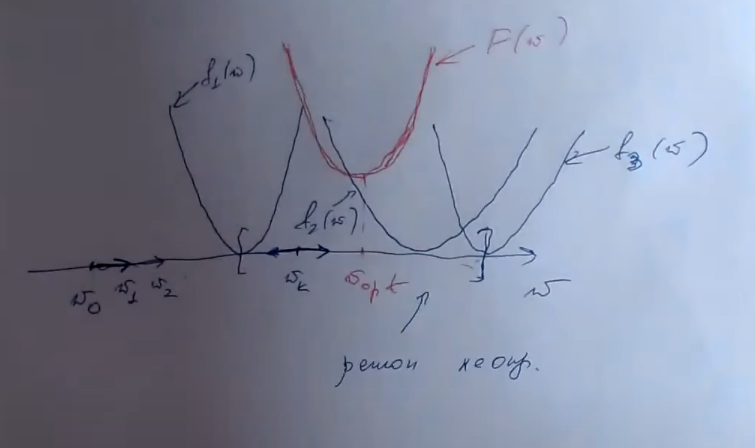
\includegraphics[width=10cm]{images/sgd.png}
\end{figure}
\\
Метод стохастического градиентного спуска вообще не является методом спуска, мы не гарантируем, что на каждой итерации значение функции уменьшится. Видно, что подходя к оптимуму мы попадаем в регион неопределенности, ведь даже в оптимальной точке наша оценка градиента $g_k$ не равна нулю, как нам того хотелось бы. Метод застревает около оптимума и начинает бесконечные колебания. У нас нет возможности оценить значение функции $F$, таким образом мы можем просто запускать метод на какое-то фиксированное число итераций, либо по каким-то косвенным признакам отслеживать (допустим в машинном обучении смотреть качество на отложенной выборке). В дальнейшем мы рассмотрим решение этой проблемы с помощью выбора длины шага и вариаций оценки градиента. Пока же предлагается оценить сходимость метода SGD.

\subsubsection{Скорость сходимости}
\[
    x_{k+1} = x_k - \alpha_k g_k, \quad \mathbb{E} \, g_k = \nabla F(x_k)
\]
Начинаем с невязки по точкам:
\[
    \| x_{k+1} - x_* \|^2 = \| x_k - \alpha_k g_k - x_* \|^2 = \| x_k - x_* \|^2 - 2\alpha_k g_k^T (x_k - x_*) + \alpha_k^2 \| g_k \|^2
\]
Теперь берем матожидание по случайности на $k-$ой итерации:
\[
    \mathbb{E}_{i_{k}} :\quad  \mathbb{E}_{i_{k}} \| x_{k+1} - x_* \|^2 = \| x_k - x_* \|^2 - 2\alpha_k \nabla F(x_k)^T (x_k - x_*) + \alpha_k^2 \mathbb{E}_{i_{k}} \| g_k \|^2
\]
Предполагаем, что $F$ - выпуклая функция, тогда:
\begin{gather*}
    F(x_*) \geq F(x_k) + \nabla F(x_k)^T (x_* - x_k) \\
    F(x_k) - F(x_*) \leq \nabla F(x_k)^T (x_k - x_*)
\end{gather*}
Теперь:
\[
    \alpha_k \nabla F(x_k)^T (x_k - x_*) = \dfrac{\| x_k - x_* \|^2}{2} + \dfrac{\alpha_k^2 \mathbb{E}_{i_{k}} \| g_k \|^2}{2} - \dfrac{\mathbb{E}_{i_{k}} \| x_{k+1} - x_* \|^2}{2}
\]
\[
    \alpha_k (F(x_k) - F(x_*)) \leq \dfrac{\| x_k - x_* \|^2}{2} + \dfrac{\alpha_k^2 \mathbb{E}_{i_{k}} \| g_k \|^2}{2} - \dfrac{\mathbb{E}_{i_{k}} \| x_{k+1} - x_* \|^2}{2}
\]
Теперь давайте возьмем матожидание по всей случайности:
\[
    \mathbb{E}: \quad \alpha_k (\mathbb{E} F(x_k) - F(x_*)) \leq \dfrac{\mathbb{E} \| x_k - x_* \|^2}{2} + \dfrac{\alpha_k^2 \mathbb{E} \| g_k \|^2}{2} - \dfrac{\mathbb{E} \| x_{k+1} - x_* \|^2}{2}
\]
Теперь просуммируем по индексам от $0$ до $k$:
\[
    \sum\limits_{i=0}^{k} \alpha_i (\mathbb{E} F(x_i) - F(x_*)) \leq \dfrac{\| x_0 - x_* \|^2}{2} + \dfrac{\sum\limits_{i=0}^{k} \alpha_i^2 \mathbb{E} \| g_i \|^2}{2} - \dfrac{\mathbb{E} \| x_{k+1} - x_* \|^2}{2}
\]
Вспоминаем, что $F$ - выпуклая, записываем неравенство Йенсена:
\[
    \mathbb{E} F\left(\overbrace{\dfrac{\sum\limits_{i=0}^{k} \alpha_i x_i}{\sum\limits_{i=0}^{k}\alpha_i}}^{\overline{x_k}}\right) - F(x_*) \leq \dfrac{\sum\limits_{i=0}^{k} \alpha_i (\mathbb{E} F(x_i) - F(x_*))}{\sum\limits_{i=0}^{k}\alpha_i} \leq \dfrac{\| x_0 - x_* \|^2 + \sum\limits_{i=0}^{k} \alpha_i^2 \mathbb{E} \| g_i \|^2}{2\sum\limits_{i=0}^{k}\alpha_i}
\]
Теперь ограничим начальную невязку как $R^2$, положим, что все $f_i \in C^{0, 0}_{G}$, тогда можно ограничить норму квадрата градиента как $G^2$:
\[
    \mathbb{E} F(\overline{x_k}) - F(x_*) \leq \dfrac{R^2 + G^2 \sum\limits_{i=0}^{k} \alpha_i^2}{2\sum\limits_{i=0}^{k}\alpha_i}
\]
Таким образом с точки зрения теоремы мы можем гарантировать что-либо только для средней точки $\overline{x_k}$, однако "если провести численные эксперименты, мы увидим, что разница не существенная". \\
Теперь рассмотрим разные стратегии выбора длины шага $\alpha_k$:

\subsubsection{Стратегии выбора длины шага}
\begin{itemize}
    \item \textbf{Константный} $\alpha_k = h$:
    \[
        \dfrac{R^2 + G^2 h^2 (k+1)}{2(k+1)h} = \dfrac{R^2}{2h(k+1)} + \dfrac{G^2 h}{2} \to_{k \to \infty} \dfrac{G^2 h}{2}
    \]
    \begin{figure}[h]
        \center
        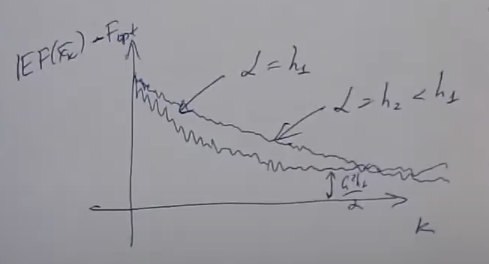
\includegraphics[width=7cm]{images/sgd2.png}
    \end{figure}
    \\
    Видно, что при меньшем шаге мы сходимся медленнее, зато в меньшее значение невязки.
    Однако это всё про матожидание, и тут на помощь нам приходит неравенство Маркова:
    \[
        \xi := F(\overline{x_k}) - F(x_*) \geq 0 \Rightarrow p\left( F(\overline{x_k}) - F(x_*) \geq a \right) \leq \dfrac{\mathbb{E}F(\overline{x_k}) - F(x_*)}{a}
    \]
    \item \textbf{Устремить к нулю $\alpha$}
    \begin{enumerate}
        \item $\sum\limits_{i=0}^{k} \alpha_i = \infty, \ \ \sum\limits_{i=0}^{k} \alpha_i^2 < \infty$
        \[
            \alpha_i = \dfrac{h}{(i + 1)^{\tau}}, \quad \tau \in \left(\dfrac{1}{2}, 1\right]
        \]
        \item $\sum\limits_{i=0}^{k} \alpha_i = \infty, \ \ \sum\limits_{i=0}^{k} \alpha_i^2 = \infty, \ \ \lim\limits_{k \to \infty}\dfrac{\sum\limits_{i=0}^{k} \alpha_i^2}{\sum\limits_{i=0}^{k} \alpha_i} = 0$
        \[
            \alpha_i = \dfrac{h}{(i + 1)^{\tau}}, \quad \tau \in \left(0, \dfrac{1}{2}\right]
        \]
    \end{enumerate}
    $\tau_{opt} = \dfrac{1}{2} \Rightarrow$ скорость сходимости будет $O\left(\dfrac{\ln(k)}{\sqrt{k}}\right) = \tilde{O}\left(\dfrac{1}{\sqrt{k}}\right)$.
\end{itemize}
Составим табличку скоростей сходимости методов и их стохастических аналогов:
\begin{center}
{\renewcommand{\arraystretch}{1.4}
\begin{tabular}{|c|c|c|c|}
    \hline
    & & \multicolumn{2}{|c|}{Скорость сходимости} \\
    \hline
    Метод          & Функция                               & Обычный                     & Стохастический              \\
    \hline
    Градиентный    & $f \in C^{1,1}_{L}$ и сильно выпуклая & $O(C^k)$                    & $O(\nicefrac{1}{k})$        \\
    \hline
    Градиентный    & $f \in C^{1,1}_{L}$ и выпуклая        & $O(\nicefrac{1}{k})$        & $O(\nicefrac{1}{\sqrt{k}})$ \\
    \hline
    Субградиентный & $f \in C^{0,0}_{L}$ и выпуклая        & $O(\nicefrac{1}{\sqrt{k}})$ & $O(\nicefrac{1}{\sqrt{k}})$ \\
    \hline
\end{tabular}
}
\end{center}
Видно, что с такой скоростью сходимости для требуемой точности необходимо огромное число итераций, хотим метод с линейной скоростью сходимости.

\subsubsection{SAG и SVRG}

\paragraph{SAG}
\begin{gather*}
    \textsc{GD}: \quad x_{k+1} = x_k - \alpha_k \dfrac{1}{n} \sum\limits_{i=1}^{n} \nabla f_i (x_k) \\
    \textsc{SAG}: \quad x_{k+1} = x_k - \alpha_k \dfrac{1}{n} \sum\limits_{i=1}^{n} \nabla f_i (v_i^k)
\end{gather*}
Пытаемся сделать так, чтобы в пределе направление оптимизации приходило в полный градиент. На каждой итерации меняем одну точку $v_i^k$. Рассмотрим итерацию метода:
\begin{algorithmic}[1]
    \Procedure{SAG}{}
        \State $i_k \gets \textsc{UNIFORM}(1, 2, \dots , n)$
        \State $v_{i_k}^k \gets x_k; v_{j}^k \gets v_{j}^{k-1} \, \forall j \neq i_k $
        \State $g_k \gets \dfrac{1}{n} \sum\limits_{i=1}^{n} \nabla f_i (v_i^k) = g_{k-1} + \dfrac{1}{n} \left(\nabla f_{i_k}(v_{i_k}^k) - \nabla f_{i_k}(v_{i_k}^{k-1})\right)$
        \State $x_{k+1} \gets x_k - \alpha_k g_k$
    \EndProcedure
\end{algorithmic}
В методе возникает память, которая имеет размер, зависящий от количества объектов: $O(nd)$. \\
Для скорости сходимости метода SAG верно следующее утверждение (оно вида теоремы, но главный по оптам сказал можно не доказывать и даже не формулировать строго):
\theorem{
Пусть $F \in C^{1,1}_{L}$ и $\mu$ сильно выпуклая, длина шага $\alpha_k = \dfrac{1}{16L}$, тогда для невязки по функции для метода SAG верна следующая оценка:
\[
    \mathbb{E} F(x_k) - F(x_*) \leq \left( 1 - \min\left( \dfrac{\mu}{16L}, \dfrac{1}{8n} \right) \right)^k C
\]
}
Имеет обратить внимание на то, что $k$ - это номер стохастической итерации, то есть он сходится быстрее градиентного спуска где-то в $n$ раз. Также у него есть возможность адаптивного подбора константы Липшица.\\
Однако он работает только для выпуклых и сильно выпуклых функций. И еще стоит обратить внимание в связи с этим методом, на то, что он оптимизирует именно сумму функций и направлен на это. То есть в более общем случае, когда мы оптимизируем функцию вида матожидание по распределению мы не можем использовать SAG:
\[
    F(x) = \mathbb{E}_{q(y)} f(x, y) \to \min\limits_{x}
\]
Ну и далее мы рассмотрим метод, похожий на SAG, однако который можно применять на более общие задачи вида выше.

\paragraph{SVRG}
Идея следующая, в какой-то точке потратить время и посчитать полный градиент функции, потом использовать его для построения оценок для $g_k$:
\begin{gather*}
    \tilde{x}: \quad \tilde{\mu} = \dfrac{1}{n} \sum\limits_{i=1}^{n} \nabla f_i (\tilde{x}) = \nabla F(\tilde{x}) \\
    g_k = \nabla f_{i_k} (x_k) - \nabla f_{i_k} (\tilde{x}) + \tilde{\mu} \\
    \mathbb{E} g_k = \mathbb{E} \nabla f_{i_k} (x_k) - \mathbb{E} \nabla f_{i_k} (\tilde{x}) + \mathbb{E} \tilde{\mu} = \nabla F(x_k)
\end{gather*}
Таким образом мы в методе совершаем итерации вида: оцениваем полный градиент в точке $\tilde{x_0}$, делаем какое-то количество стохастических итераций, оцениваем полный градиент в точке $\tilde{x_1}$ и так далее. Его можно применять для общих функций вида матожидание по распределению, у него есть теорема аналогичная как для SAG, что он сходится линейно с константным шагом обратно пропорциональным константе Липшица, у него есть критерий останова связанный с нормой $\tilde{\mu}$ и у него есть возможность адаптивного подбора константы Липшица, то есть его можно запускать что называется "из коробки".

    \subsection{Риманова оптимизация, её основные компоненты (риманово многообразие, касательное пространство, римановый градиент, операции ретракции и транспортировки вектора). Римановый градиентный спуск, примеры применения. Примеры римановых многообразий. @isadrtdinov}

    Прежде всего возникает вопрос: а зачем вообще нам нужны нетрадиционные методы оптимизации, раз мы уже разобрали градиентные спуски на любой вкус и цвет, методы Ньютона и прочая, и прочая, и прочая? Дело в том, что разобранные нами методы для условной оптимизации подходят не для всех множеств (например, мы можем захотеть оптимизировать функцию $f(x)$ по шару $x^T x = 1$, а метод барьеров не умеет работать с множествами без внутренности).

Рассмотрим еще один простой пример. Частая проблема в рекуррентных сетях - затухание градиента (когда норма весов $\|W\| < 1$) или взрыв градиента (соответствено, $\|W\| > 1$). Хорошей практикой здесь считается брать матрицу весов $W$ ортогональной, что позволяет контролировать ее норму (она становится единичной). Прелесть римановской оптимизации в том, что она позволяет оптимизировать функции по очень сложным множествам (типа множества ортогональных матриц или шара без внутренности).

Центральным понятием в римановской оптимизации явлется риманов градиент. Рассмотрим ради простоты всю конструкцию на сфере $S^{n-1}$. Рассмотрим некоторую точку сферы $x$ и ее окрестность. \textbf{Римановым градиентом} $\grad f(x)$ называется направление кривой наибольшего возрастания в окрестности точки $x$. Он представляет собой вектор, лежащий в касательной плоскости к сфере в точке $x$.

Казалось бы все, наши проблемы решены! Берем и делаем шаг вдоль направления риманова антиградиента. Но есть проблема: такой шаг выведет нас за пределы нашего множества:

$$
x_{k+1} = x_k - \alpha_k \grad f(x_k) \not\in S^{n-1}
$$

\noindent
Нам нужно как-то шагнуть в сторону уменьшения функции, но при этом остаться на сфере. Для этого вводится операция \textbf{ретракции} - это в некотором смысле проецирование риманова градиента на наше множества. По итогу, чтобы задать риманов градиентный спуск (RGD), нам нужно определить риманов градиент и операцию ретракцию.

$$
x_{k+1} = R_{x_k}\big(-\alpha_k \grad f(x_k)\big)
$$

\begin{figure}[H]
    \centering
    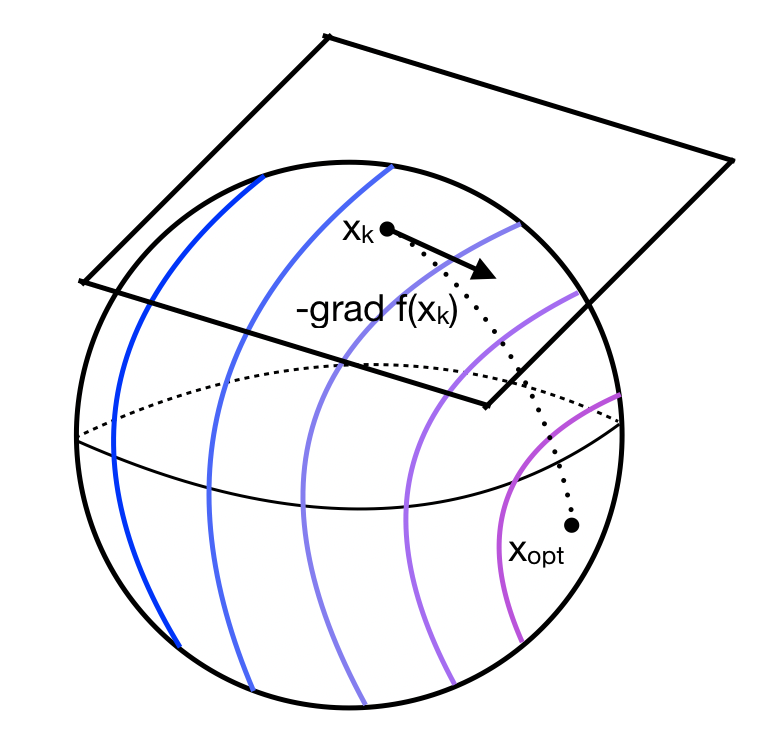
\includegraphics[width=8cm]{images/2-14-sphere.png}
    \caption{Риманов антиградиент в точке $x_k$. Цветными кривыми показаны линии уровня функции $f(x)$.}
    \label{fig:my_label}
\end{figure}

Теперь перейдем к формализму (наверное, правильнее начинать рассказывать билет отсюда, а все, что выше, приведено для понимания общей логики происходящего).

\textbf{Многообразием} $M$ размерности $d$ называется множество, удовлетворяющее двум свойствам:

\begin{enumerate}
    \item $\forall x \in M, U$ - открестность $x$ $\exists$ отображение $\phi: U \rightarrow \R^d$, биективно переводящее $U$ в некоторое открытое множество. Пара $(U, \phi)$ называется картой множества $M$.
    \item Для карт $(U, \phi), (W, \psi)$ в точке $x: U \cap W \ne \O$ отображения $\phi \circ \psi^{-1}$ и $\psi \circ \phi^{-1}$ дифференцируемы бесконечное число раз как функции $\R^d \rightarrow \R^d$.
\end{enumerate}

При этом $\phi(x) \in \R^d$ называются локальными координатами, а если $M \subset \R^n$, то $x \in \R^n$ называются глобальными координатами.

\underline{Примеры многообразий}:

\begin{enumerate}
    \item Окружность $S^1 = \{(x_1, x_2): x_1^2 + x_2^2 = 1\}$. Тогда $t \in [0, 2\pi)$ - это локальные координаты, а в качестве отображения $\phi(x)$ можно взять подходящую обратную тригонометрическую функцию.
    \item Все пространство $\R^n$. В качестве биекции берем тривиальную, а локальные координаты совпадают с глобальными.
    \item Манифолд Штифеля $\text{St}(m, n) = \{X \in \R^{n \times m} \big| X^T X = I_m\}$ (в сущности, множество ортогональных матриц).
\end{enumerate}

\textbf{Касательным пространством} в точке $x \in M$ называется множество $T_x M = \{\xi \in \R^n \big| \xi = \gamma'(0), \text{ где } \gamma(t) - \text{ это кривая в } M \text{ и } \gamma(0) = x\}$. По сути, это множество всех направлений кривых на $M$ в точке $x$.

Для примера найдем касательное пространство для шара $S^{n-1} = \{x \in \R^n \big| x^T x = 1\}$ в точке $x_0$. Интересующее нас множество кривых выглядит так:

$$
\begin{cases}
    x(t)^T x(t) = 1 \\
    x(0) = x_0
\end{cases}
$$

\noindent
Продифференцируем первое уравнение по $t$ и подставим $t=0$:

$$
x'(0)^T x(0) + x(0)^T x'(0) = 0 \Rightarrow x'(0)^T x_0 = 0
$$

\noindent
Обозначим $U_{x_0} = \{z | z^T x_0 = 0\}$. Мы только что доказали, что $T_{x_0} S^{n-1} \subseteq U_{x_0}$. Осталось показать обратное вложение. Пусть $x(t) = \frac{x_0 + tz}{\|x_0 + tz\|}$. Утверждение $x(0) = x_0$ тривиально. Нужно проверить, что $x'(0) = z$:

$$
x^i(t) = \frac{x_0^i + tz^i}{\|x_0 + tz\|}
$$

$$
x^i(t)' = \frac{z^i \|x_0 + tz\| - (x_0^i + tz^i) \frac{2\sum_{j=1}^n (x_0^j + t z^j)z^j}{2\|x_0 + tz\|}}{\|x_0 + tz\|^2} = z^i \frac{1}{\|x_0 + tz\|} - (x_0^i + tz^i) \frac{z^T (x_0 + tz)}{\|x_0 + tz\|^3}
$$

$$
x^i(0)' = z^i - x_0^i z^T x_0 = z^i
$$

\noindent
Таким образом, $x'(0) = z$, а значит, $U_{x_0} \subseteq T_{x_0} S^{n-1}$, и поэтому $T_{x_0} S^{n-1} = U_{x_0}$. Мы получили, что касательное простанство к шару - это множество векторов, перпендикулярных радиусу, что логично. Тут нужно сделать еще два важных замечания:

\begin{enumerate}
    \item $T_x M$ - линейное подпространство
    \item $\Dim T_x M = \Dim M$
\end{enumerate}

Теперь мы готовы ввести центральное понятие. \textbf{Римановым многообразием} называется многообразие $M$, снабженное скалярным произведением на каждом касательном пространстве $T_x M$, его принято обозначать $g_x(\cdot, \cdot) = \langle \cdot, \cdot \rangle_x$. Если $M \subset \R^n$, то в качестве скалярного произведение удобно брать стандартное евклидово.

\textbf{Производной по направлению} $\xi$ в римановском случае называется
$$
D f(x) [\xi] = \frac{df(\gamma(t))}{dt} \bigg|_{t = 0}, \text{ где } \gamma(t) - \text{ кривая в } M: \gamma(0) = x, \gamma'(0) = \xi
$$

\textbf{Римановым градиентом} называется вектор $\grad f(x)$, для которого верно следующее:

$$
\big\langle \grad f(x), \xi \big\rangle_x = D f(x) [\xi], \forall \xi \in T_x M
$$

\noindent
Для градиента верно соображение про максимальное направление роста функции на множестве. В частности, верно следующее (здесь нормы берутся по скалярному произведению из определения риманова многообразия):

$$
\frac{\grad f(x)}{\|\grad f(x)\|} = \argmax_{\xi \in T_x M: \|\xi\| = 1} D f(x) [\xi]
$$

\noindent
При этом, если $M \subset \R^n$, то $\grad f(x) = P_{T_x M} (\nabla f(x))$. Поскольку $T_x M$ - линейное подпространство в $\R^n$, то можно написать $\nabla f(x) = P_{T_x M} (\nabla f(x)) + P_{{T_x M}^\bot} (\nabla f(x))$. Тогда:

$$
\big\langle P_{T_x M} (\nabla f(x)), \xi \big\rangle_x = \Big\langle \nabla f(x) - P_{{T_x M}^\bot} (\nabla f(x)), \xi \Big\rangle_x = \big\{\xi \in T_x M\big\} = \big\langle \nabla f(x), \xi \big\rangle_x = D f(x) [\xi]
$$

\noindent
В последнем равенстве мы получили производную по направлению в евклидовом смысле, но поскольку $\xi \in T_x M$, то она совпадает с римановской. Отсюда $\grad f(x) = P_{T_x M} (\nabla f(x))$.

Обозначим $TM = \bigcup_{x \in M} (x, T_x M)$. \textbf{Ретракцией} называется отображение $R: TM \rightarrow M$ ($R_x: T_x M \rightarrow M$), удовлетворяющее двум свойствам:

\begin{enumerate}
    \item $R_x(0) = x$
    \item $\displaystyle\frac{dR_x(t\xi)}{dt} = \xi, \forall \xi \in T_x M$
\end{enumerate}

\underline{Пример}:
\begin{enumerate}
    \item $S^{n-1}$: $R_x(\xi) = \frac{x + \xi}{\|x + \xi\|}$ (доказательство полностью аналогично примеру про касательное пространство).
    \item $\text{St}(m, n)$: $R_X(\Xi) = (X + \Xi) (I_m + \Xi^T \Xi)^{-1/2}$
\end{enumerate}

\noindent
В общем случае поиск ретракции - это очень нетривиальная задача. В частоности, ретракция определена не единственным образом. Периодически выходят статьи с предложениями разных операторов ретракции.

Теперь мы можем с чистой совестью определить RGD: $x_{k+1} = R_{x_k} (-\alpha_k \grad f(x_k))$. Но мы пойдем дальше и выпишем формулы для RGD с моментумом. Получается система:

$$
\begin{cases}
    d_{k+1} = \beta d_k + \alpha_k \grad f(x_k) \\
    x_{k+1} = R_{x_k} (-d_{k+1})
\end{cases}
$$

\noindent
Видите проблему? Нет? А она есть. Дело в том, что векторы $d_k$ и $\grad f(x_k)$ лежат в разных касательных пространствах ($d_k \in T_{x_{k-1}} M, \grad f(x_k) \in T_{x_k} M$), потому складывать их некорректно. Чтобы избежать этой проблемы, вводится операция транспортировки векторов. \textbf{Транспортировкой} вектора $\xi$ вдоль вектора $\eta$ ($\xi, \eta \in T_x M$) называется отображение $\Transp: TM \times TM \rightarrow TM$, обладающее следующими свойствами:

\begin{enumerate}
    \item $\exists R_x: \Transp_\eta (\xi) \in T_{R_x(\eta)} M$
    \item $\Transp_0 (\xi) = \xi$
    \item $\Transp_\eta (a \xi + b \zeta) = a\Transp_\eta (\xi) + b\Transp_\eta (\zeta)$
\end{enumerate}

Теперь более понятно о том, что только что произошло. Пусть у нас есть векторы $\xi$ и $\eta$ из касательного пространства точки $x$. Мы хотим сместиться из точки $x$ в точку $R_x (\eta)$, но при этом ''забрать с собой'' вектор $\xi$, чтобы он из старого касательного пространства перешел в новое. Для этого и нужна операция транспортировки. Как правило, сначала фиксируют ретракцию, а транспортировку по ней строят так:

$$
\Transp_\eta (\xi) = \frac{d}{dt} R_x (\eta + t\xi) \Big|_{t=0}
$$

\noindent
Для шара $S^{n-1}$ и ретракции $R_x (\xi) = \frac{x + \xi}{\|x + \xi\|}$ транспортировка выглядит так:

$$
\Transp_\eta (\xi) = \frac{1}{\|x+\eta\|} \Big(I_n - \frac{(x+\eta)(x+\eta)^T}{\|x+\eta\|^2} \Big) \xi
$$

Теперь мы можем написать правильные формулы для RGD+momentum. Они выглядят так:

$$
\begin{cases}
    d_{k+1} = \Transp_{-d_k} \big( \beta d_k \big) + \alpha_k \grad f(x_k) \\
    x_{k+1} = R_{x_k} (-d_{k+1})
\end{cases}
$$

\noindent
Стоит отметить, что для римановской оптимизации существуют и алгоритмы линейного поиска, и методы второго порядка, но \textbf{к счастью}, это выходит за пределы нашего курса.


\end{document}